\documentclass{article}

\usepackage[utf8]{inputenc}
\usepackage[top=0.25in,bottom=0.25in,left=0.25in,right=0.25in]{geometry}
\usepackage{float}
\usepackage{graphicx}
\usepackage{epstopdf}
\usepackage{verbatim}
\usepackage{amssymb}

% Start the document
\begin{document}

\noindent{\huge {\bf How is CCM useful?}}

\noindent\makebox[\linewidth]{\rule{\paperwidth}{0.4pt}}
\section{Linear Example \#1}
Consider the linear example dynamical system of
\begin{eqnarray}
X_t &=& \sin(t)\\
Y_t &=& AX_{t-1}+B\eta_t,
\end{eqnarray}
with $A,B\in\mathbb{R}\ge 0$ and $\eta_t\sim\mathcal{N}\left(0,1\right)$.  Specifically, consider $A,B\in[0,10]$ step through in increments of 0.1.  Figure \ref{fig1} shows $C_{XY}$ and $C{YX}$.  
\begin{center}
\begin{figure}[H]
\begin{tabular}{cc}
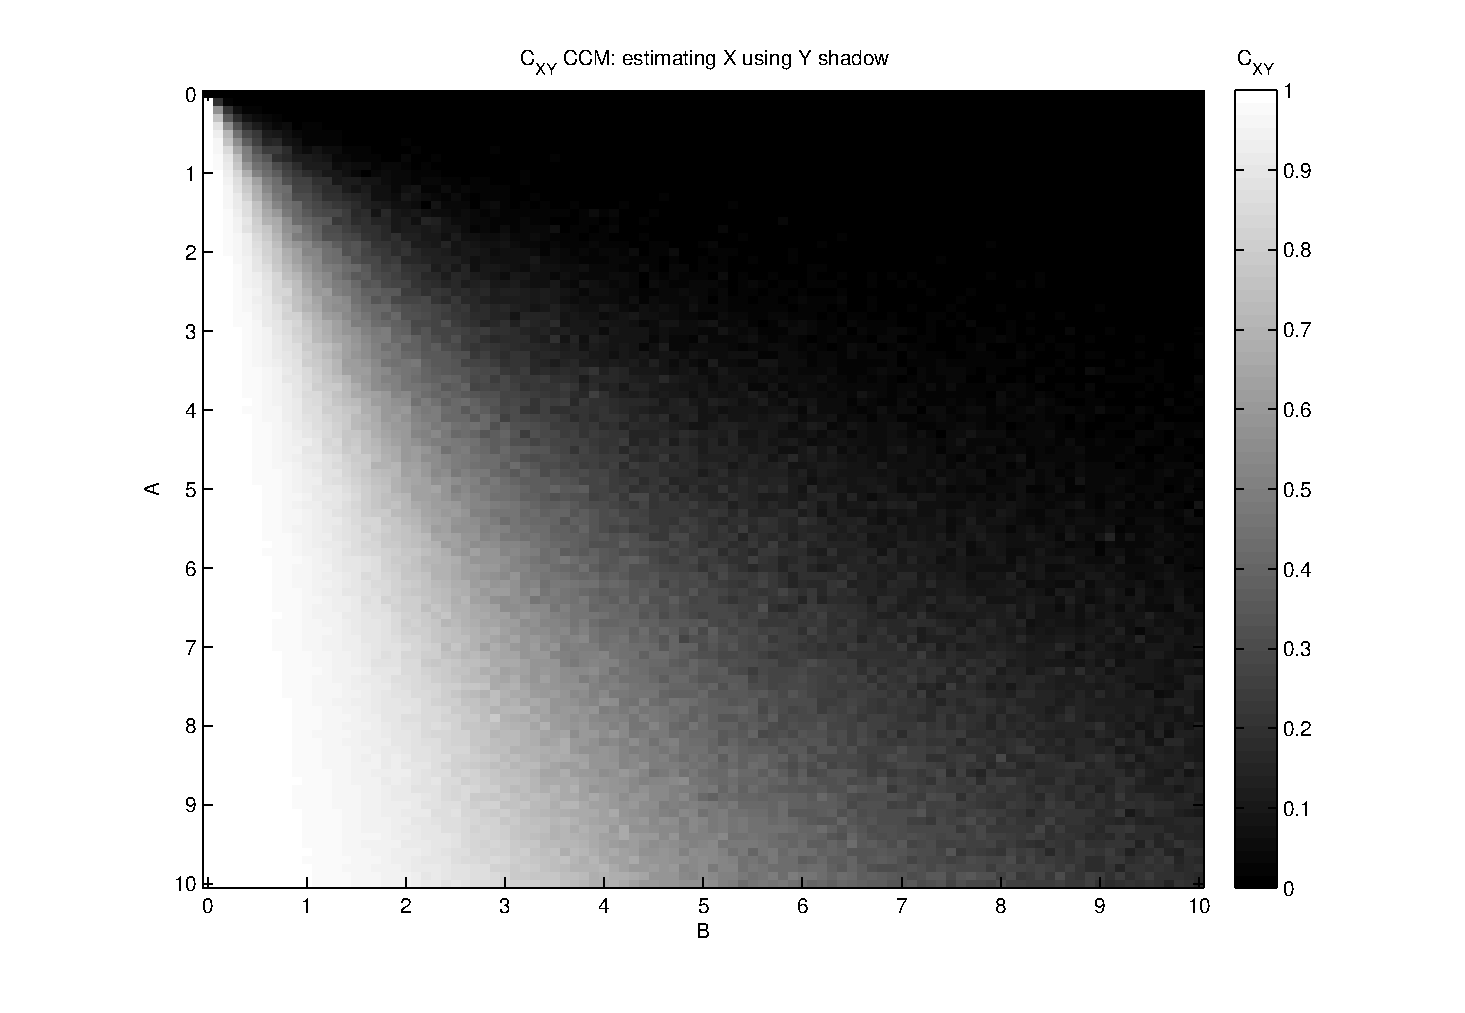
\includegraphics[scale=0.5]{LinearEx_CXY.eps} \\
(a) $C_{XY}$ \\[6pt]
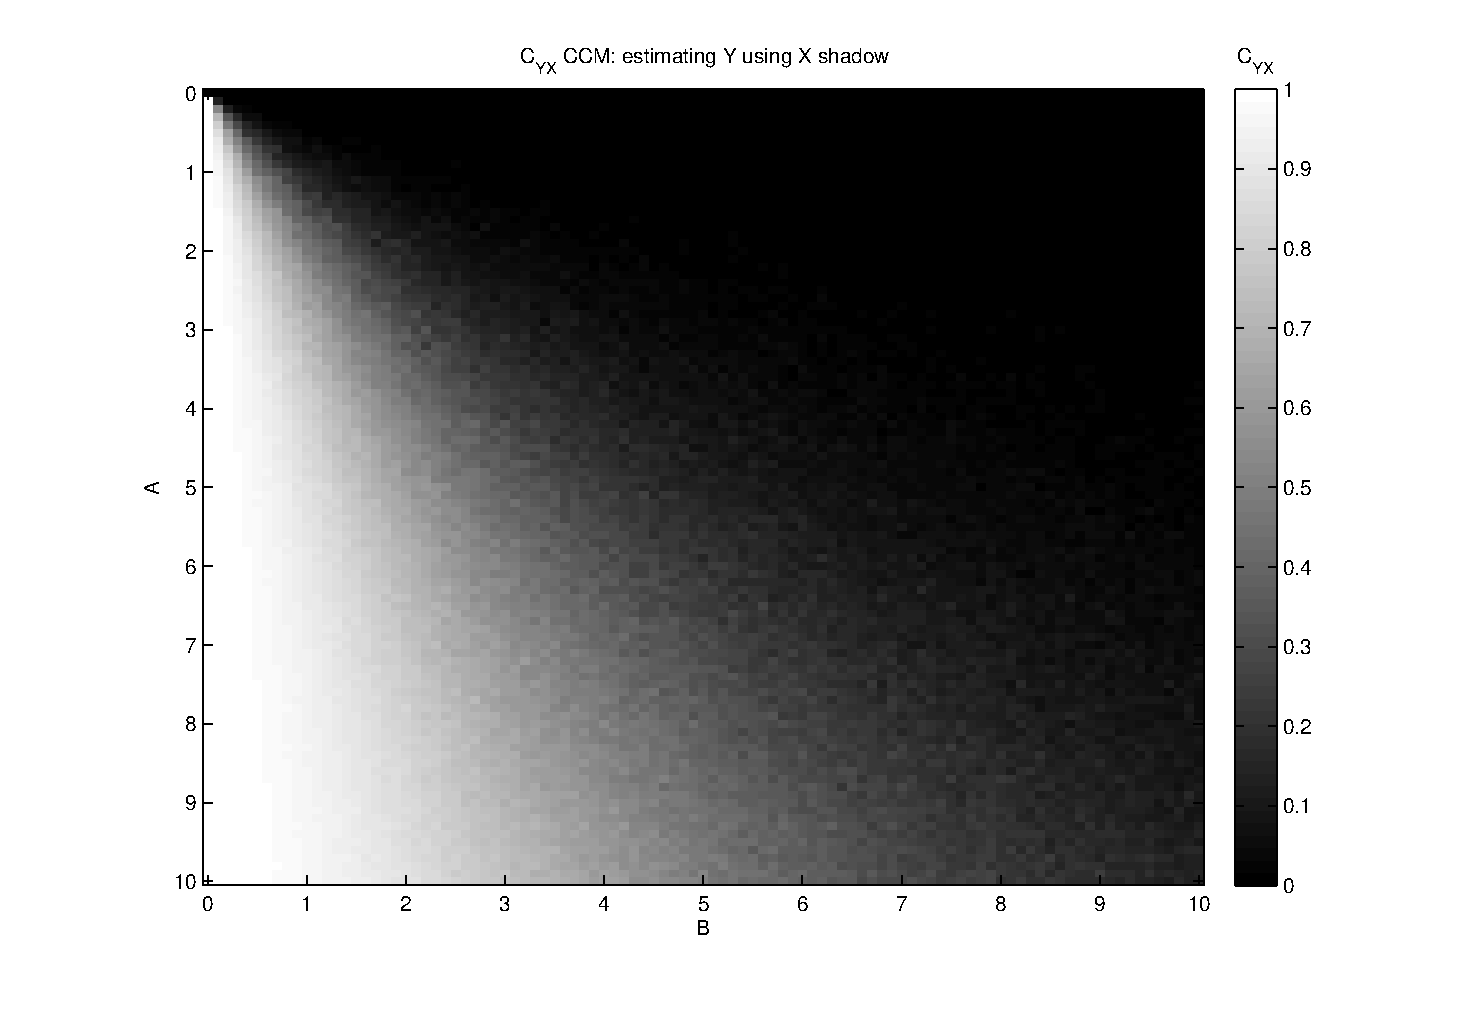
\includegraphics[scale=0.5]{LinearEx_CYX.eps} \\
(b) $C_{YX}$ \\[6pt]
\end{tabular}
\caption{Changing $A$ and $B$.  $C_{XY}$ and $C_{YX}$}
\label{fig1}
\end{figure}
\end{center}
Figure \ref{fig2} shows $\Delta$ for this example.
\begin{center}
\begin{figure}[H]
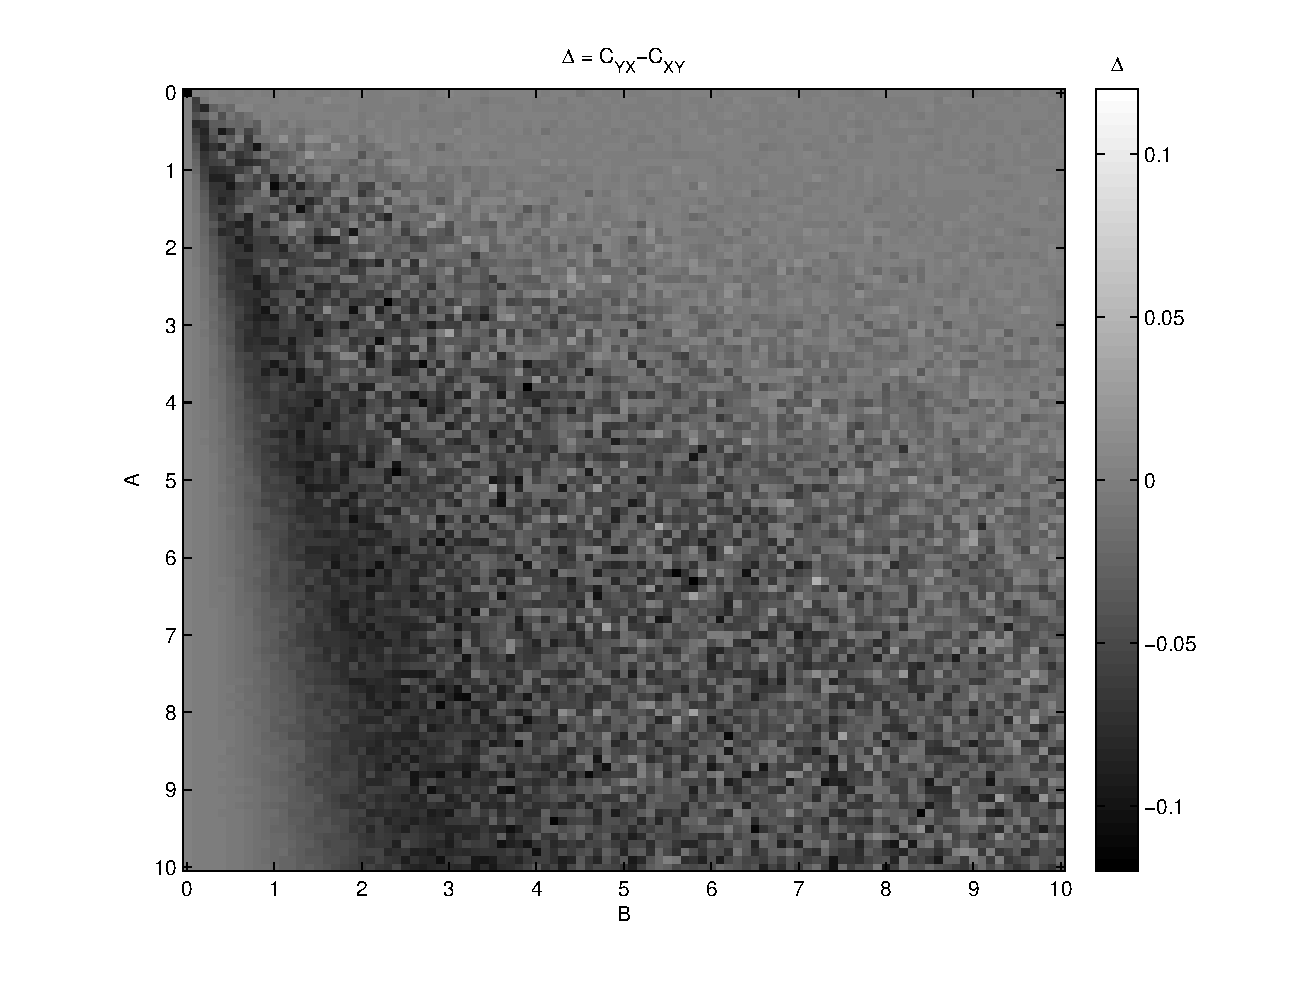
\includegraphics[scale=0.7]{LinearEx_Delta.eps} \\
\caption{Changing $A$ and $B$. $\Delta$}
\label{fig2}
\end{figure}
\end{center}
Consider the convergence of two specific points in the above plots $(A,B) = (2.6,2.6)$ and $(A,B)=(3.0,2.6)$.
\begin{center}
\begin{figure}[H]
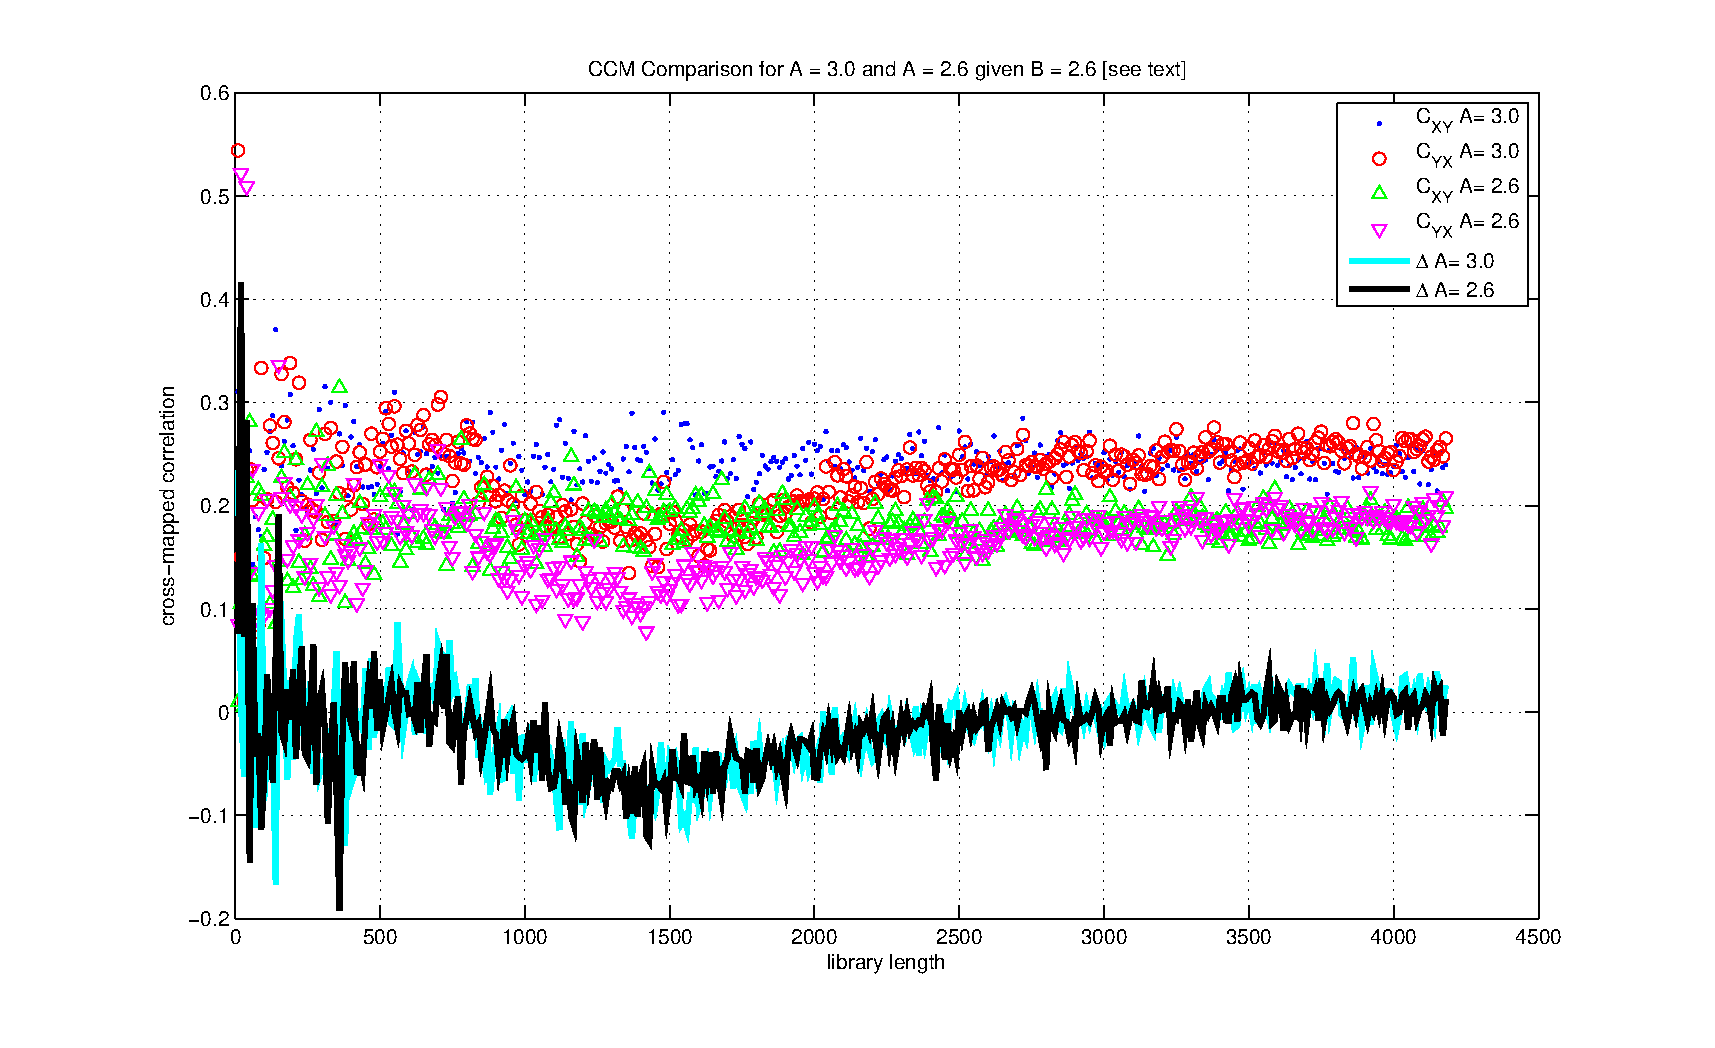
\includegraphics[scale=0.7]{LinearEx_ChangeL.eps} \\
\caption{}
\label{fig2}
\end{figure}
\end{center}

\section{Linear Example \#2}
Consider the linear example dynamical system of
\begin{eqnarray}
X_t &=& \sin(t)\\
Y_t &=& AX_{t-1}+B\eta_t\\
Z_t &=& Y_{t-1},
\end{eqnarray}
with $A,B\in\mathbb{R}\ge 0$ and $\eta_t\sim\mathcal{N}\left(0,1\right)$.  Specifically, consider $A,B\in[0,5]$ step through in increments of 0.1.    
\begin{figure}[H]
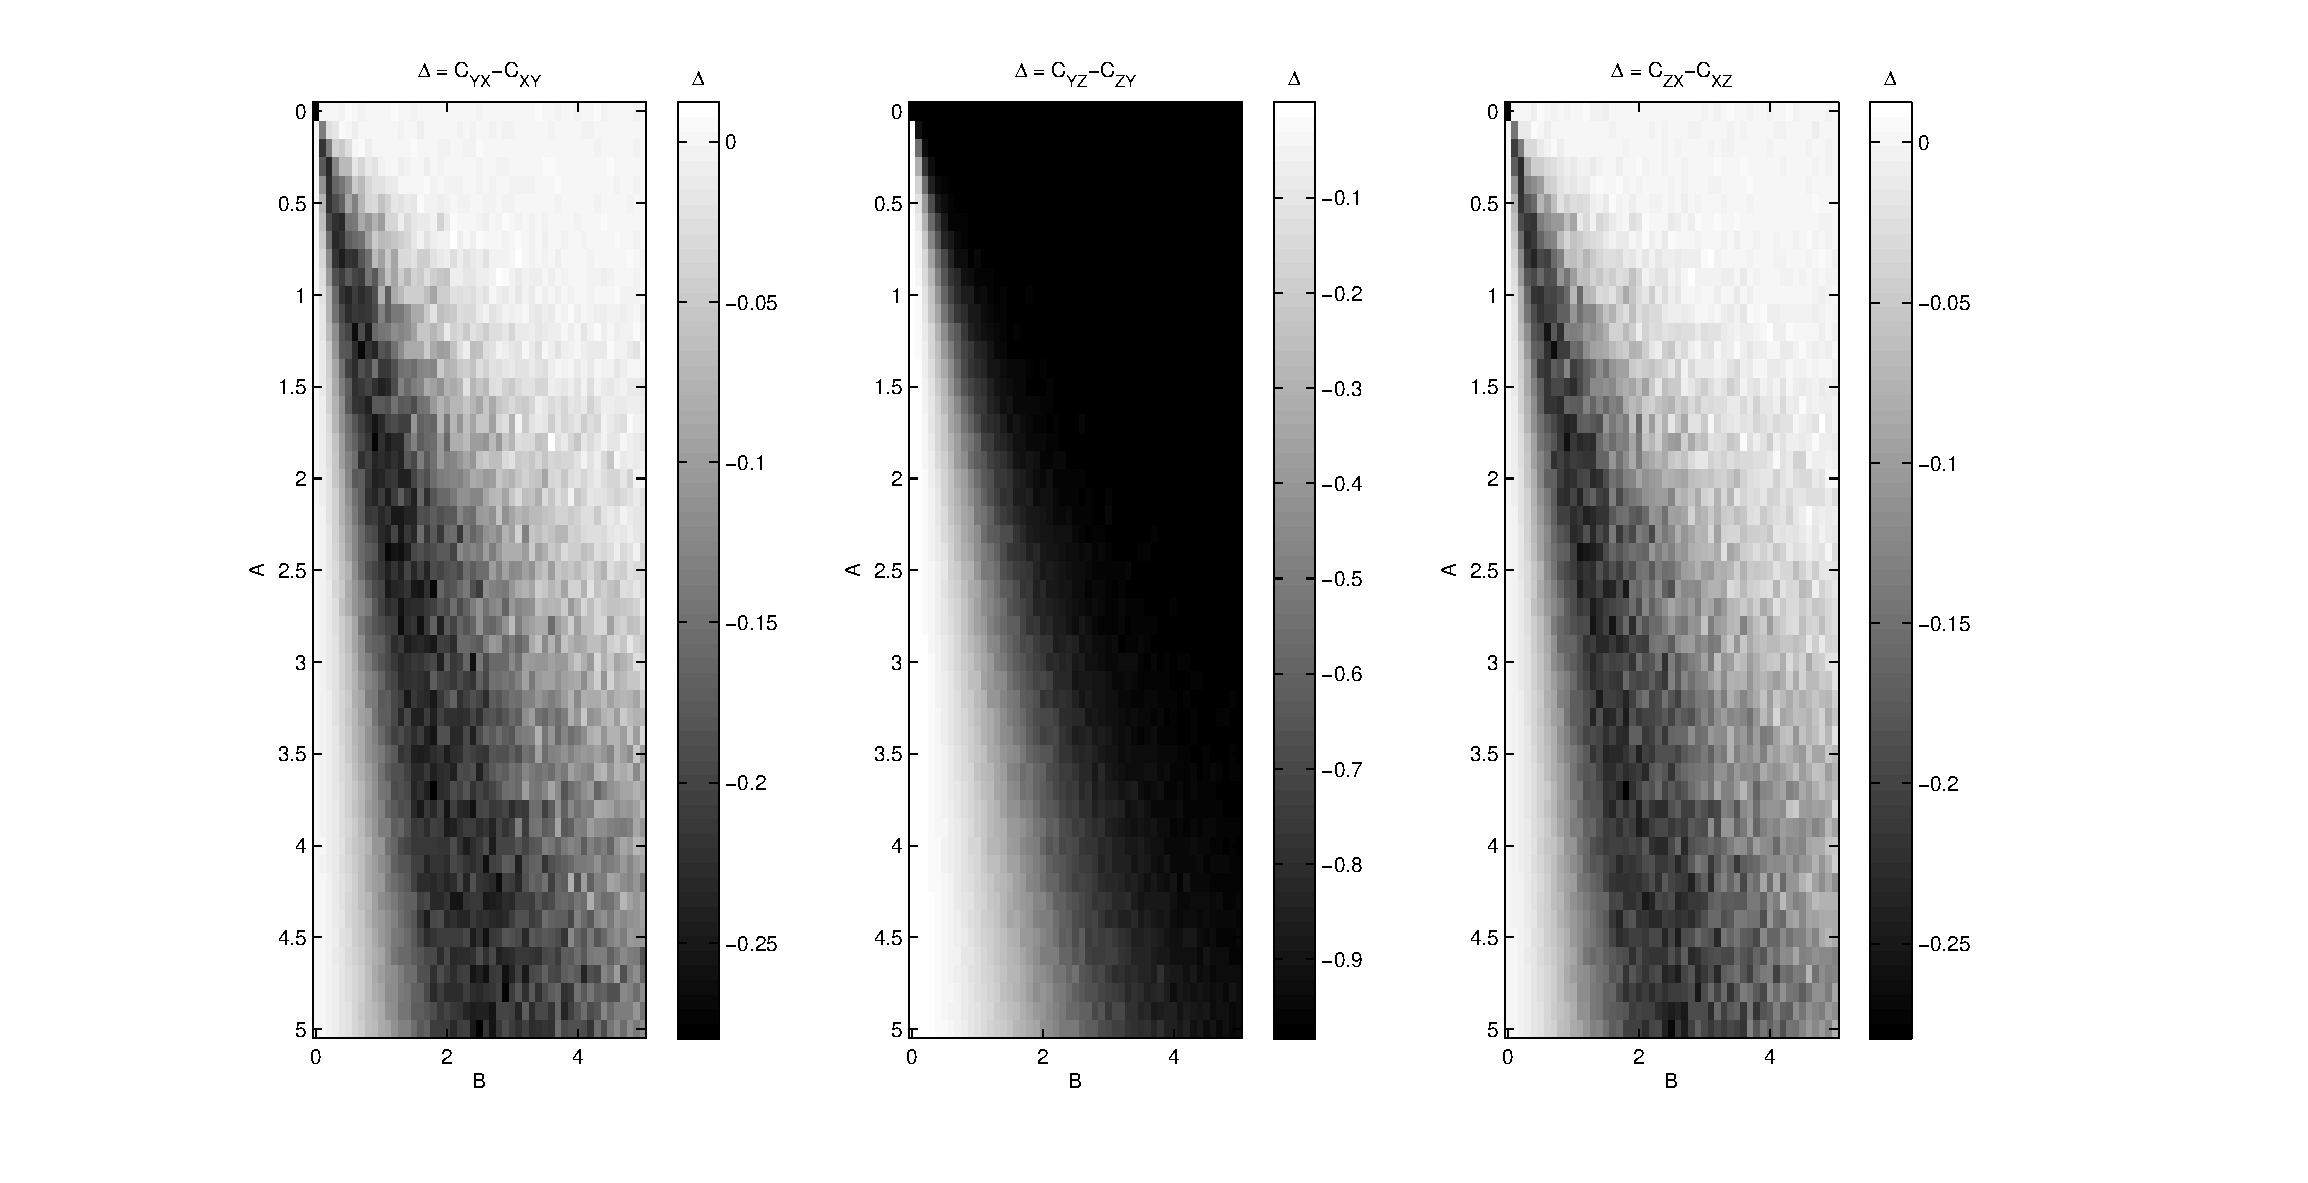
\includegraphics[scale=0.6]{LinearXYZEx.eps} \\
\caption{}
\label{fig2}
\end{figure}

\section{Non-Linear Example}
Consider the nonlinear example dynamical system of
\begin{eqnarray}
X_t &=& \sin(t)\\
Y_t &=& AX_{t-1}\left(1-BX_{t-1}\right)+C\eta_t,
\end{eqnarray}
with $A,B,C\in\mathbb{R}\ge 0$ and $\eta_t\sim\mathcal{N}\left(0,1\right)$.  Specifically, consider $A,B,C\in[0,5]$ step through in increments of 0.5.    
\begin{figure}[H]
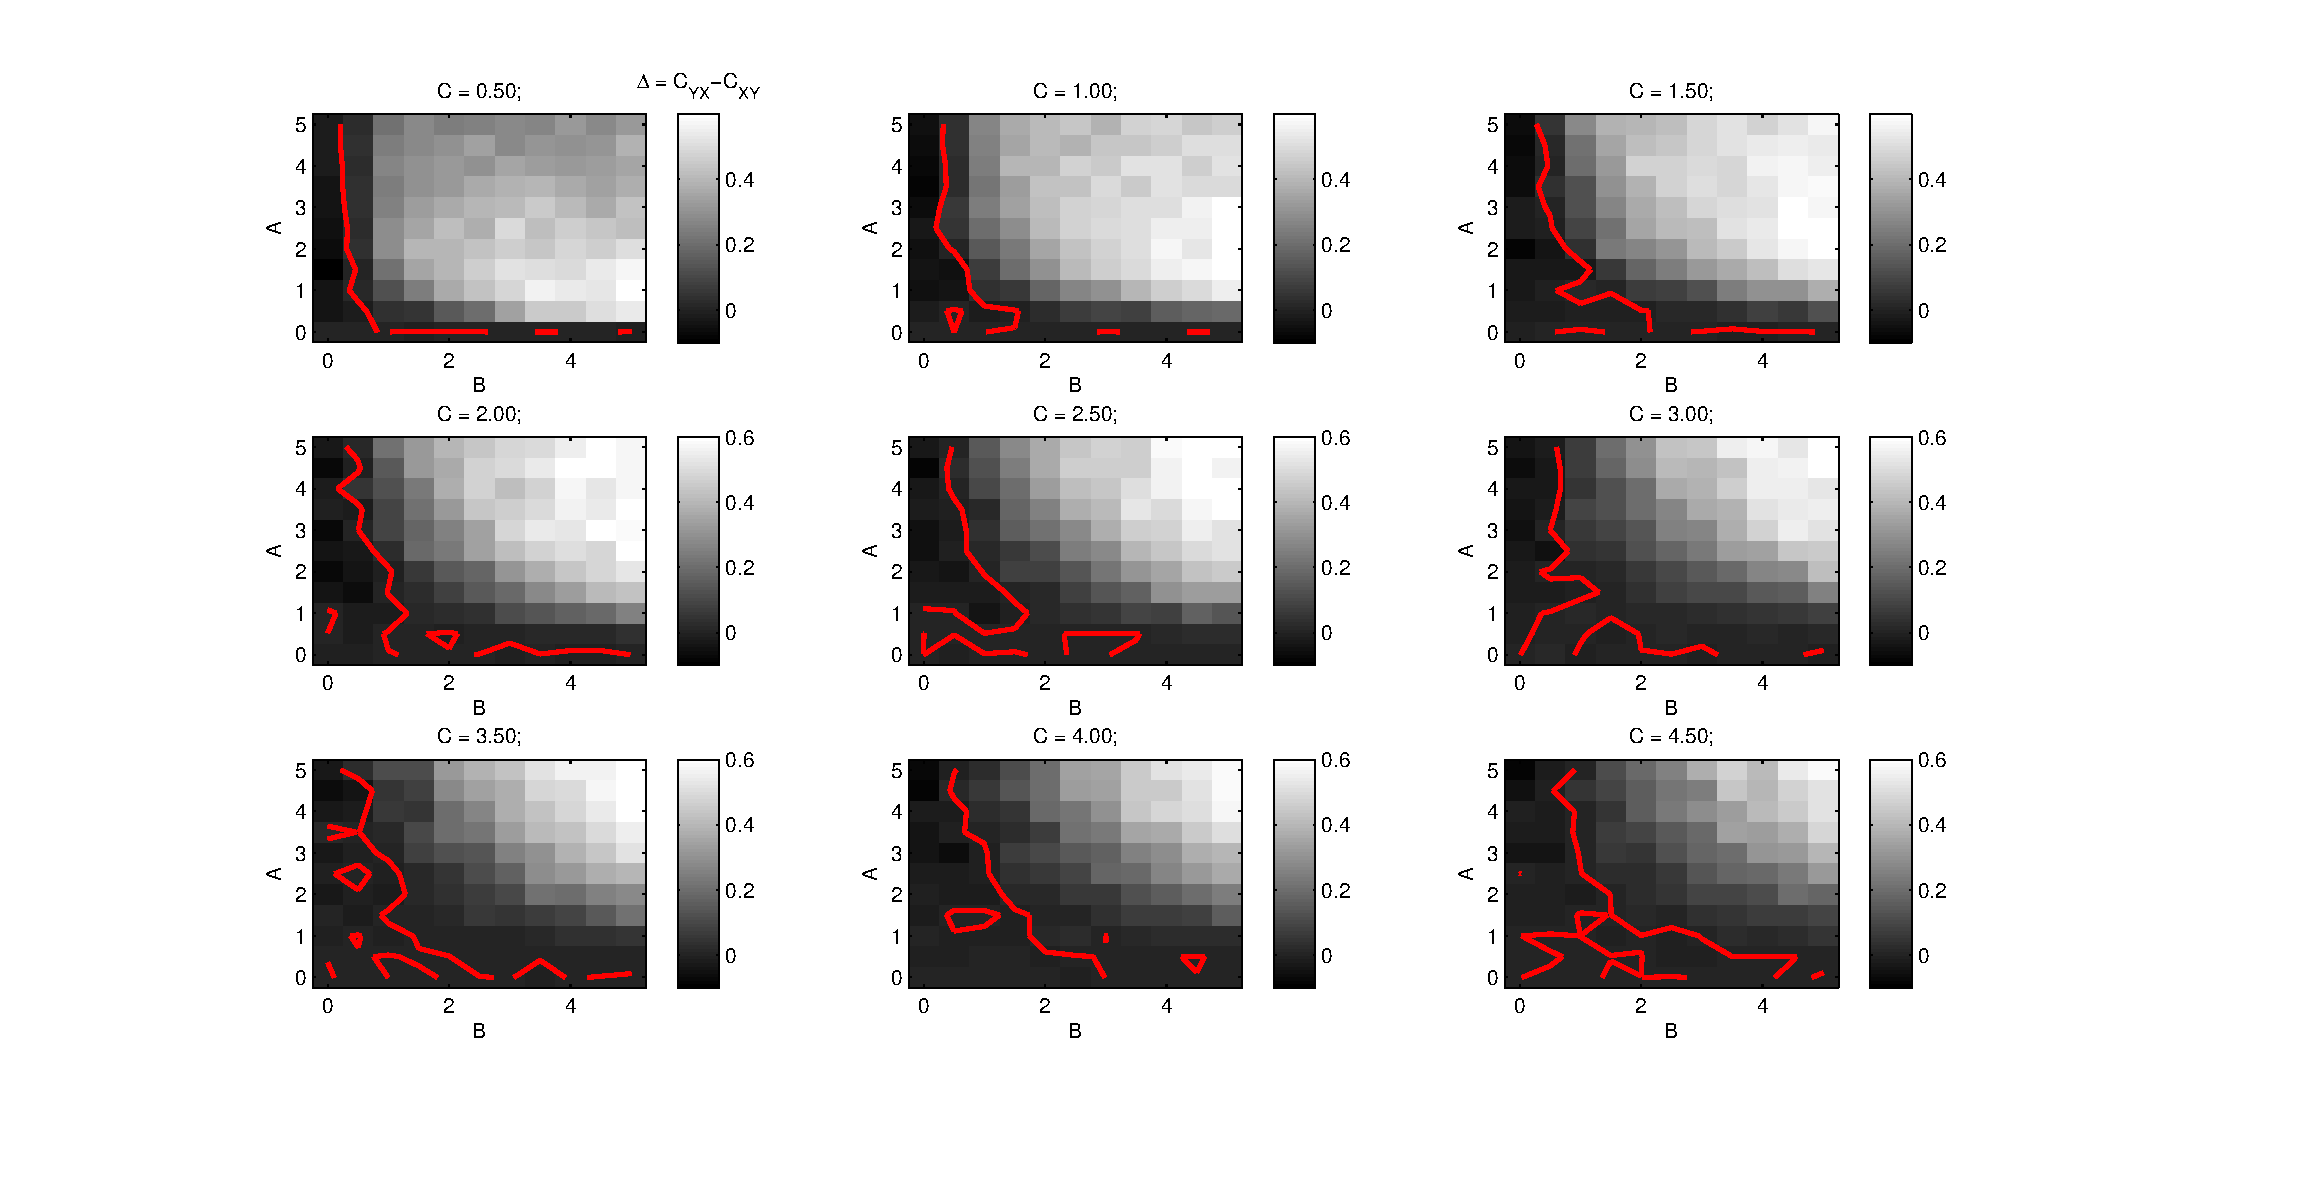
\includegraphics[scale=0.6]{NonLinearEx.eps} \\
\caption{}
\label{fig2}
\end{figure}

---
\section{RL Circuit Example}
The continuous system is
\begin{equation}
\label{eqn:it}
\frac{dI}{dt} = \frac{V(t)}{L} - \frac{R(t)}{L} I,
\end{equation}
where $I$ is the current at time $t$, $V(t)$ is the voltage at time $t$, $R(t)$ is the resistance at time $t$, and $L$ is the inductance (which is also constant in these examples), and it can be approximated as
\begin{equation}
\dot{I} = \frac{V(t)}{L} - \frac{R(t)}{L} I\Rightarrow I_{t+1}-I_t = \frac{V_t}{L} - \frac{R_t}{L} I_t.
\end{equation}
Rearranging leads to
\begin{eqnarray}
I_{t+1} &=& \frac{V_t}{L}+I_t\left(1-\frac{R_t}{L}\right),\\
V_t &=& L\left(I_{t+1}-I_t\left(1-\frac{R_t}{L}\right)\right),
\end{eqnarray}
and
\begin{equation}
R_t = L\left(I_t-I_{t+1}+\frac{V_t}{L}\right).
\end{equation}
All of the plots of $I$ seen below are produced by using MATLAB's {\em ode45} to solve Eqn. \ref{eqn:it} (i.e.\ not using the discrete approximation shown).  The time series $V(t)$ and $R(t)$ are created by defining values at fixed points and using linear interpolation (i.e.\ MATLAB's {\em interp1}) to find the time steps required by the ODE solver (i.e.\ MATLAB's {\em ode45}).  

\section{Changing V(t)}
Consider the situation where $R(t)$ is constant.
\begin{center}
{\large {\bf Physical intuition is that $V$ drives $I$, so we expect to find $V$ CCM causes $I$ ($C_{VI}>C_{IV}$).}}
\end{center}
For this example, the voltage is described by 
\begin{equation}
V(t) = A_v \sin\left(f_v t+\phi_v\right)+O_v,
\end{equation}
where $A_v$ is the amplitude, $f_v$ is the frequency, $\phi_v$ is the phase, and $O_v$ is the offset voltage.

\subsection{Changing $A_v$}
Consider evaluating the CCM correlations $C_{VI}$ and $C_{IV}$ for each $A_v\in[0.01,2.0]$ in steps of $0.01$.  For reference, both V(t) and I(t) are plotted for different $A_v$ in Figure \ref{fig:Avref}.
\begin{figure}[H]
%\includegraphics{}
\caption{Reference plots for changing $A_v$.}
\label{fig:Avref}
\end{figure}

The CCM correlations are each plotted in Figure \ref{fig:Av} along with the corresponding PAI elements $P_\theta$ and $|P|$.
\begin{figure}[H]
\begin{tabular}{cc}
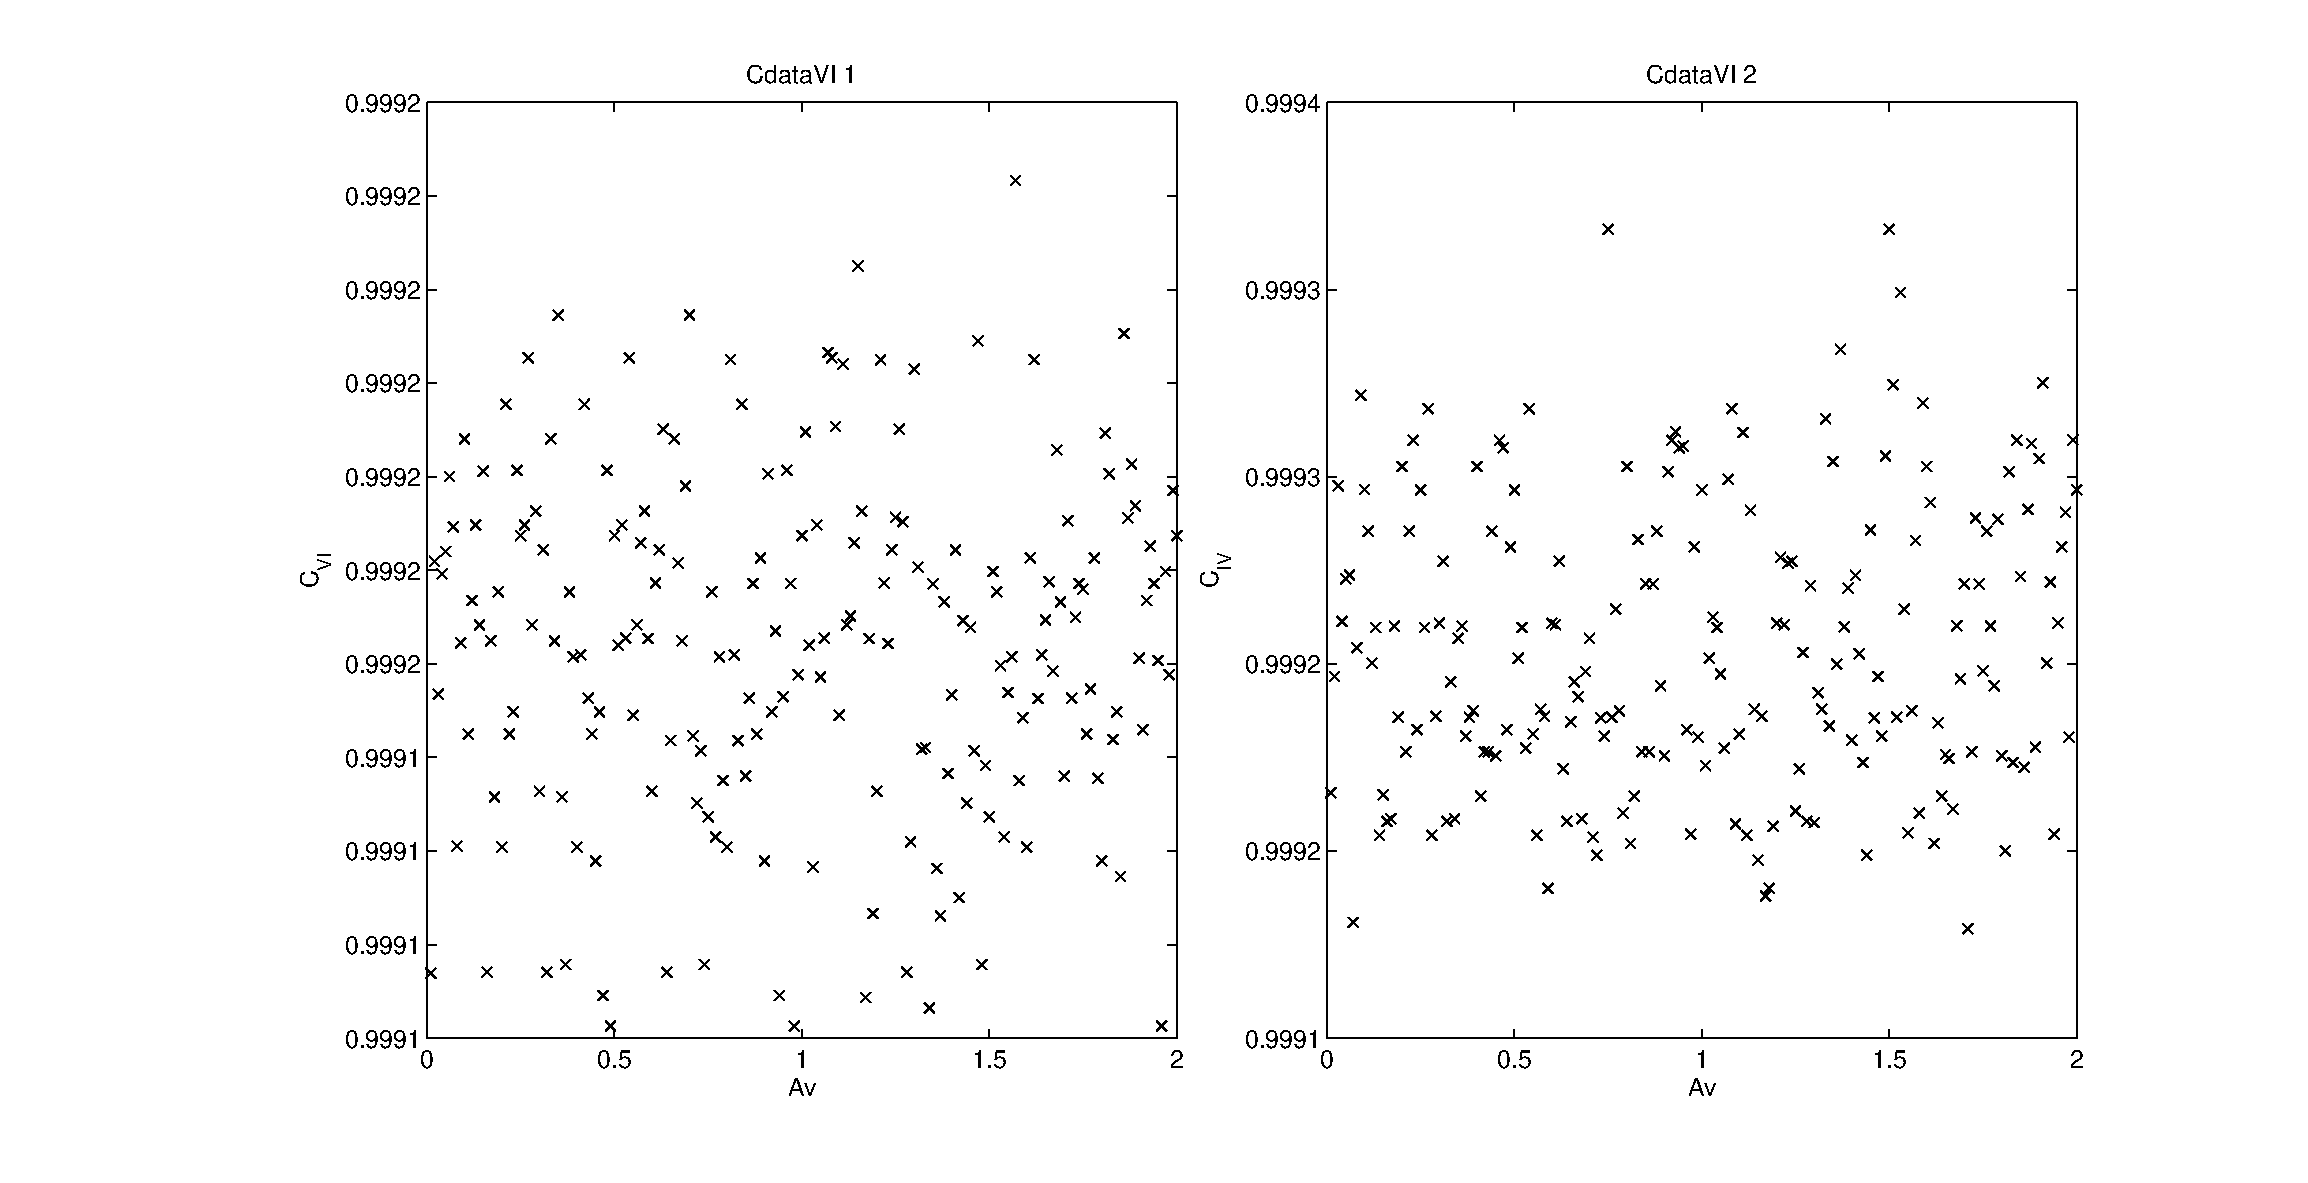
\includegraphics[scale=0.5]{RLcirc_varyV_amp2.eps} \\
(a) $C_{VI}$ and $C_{IV}$ \\[6pt]
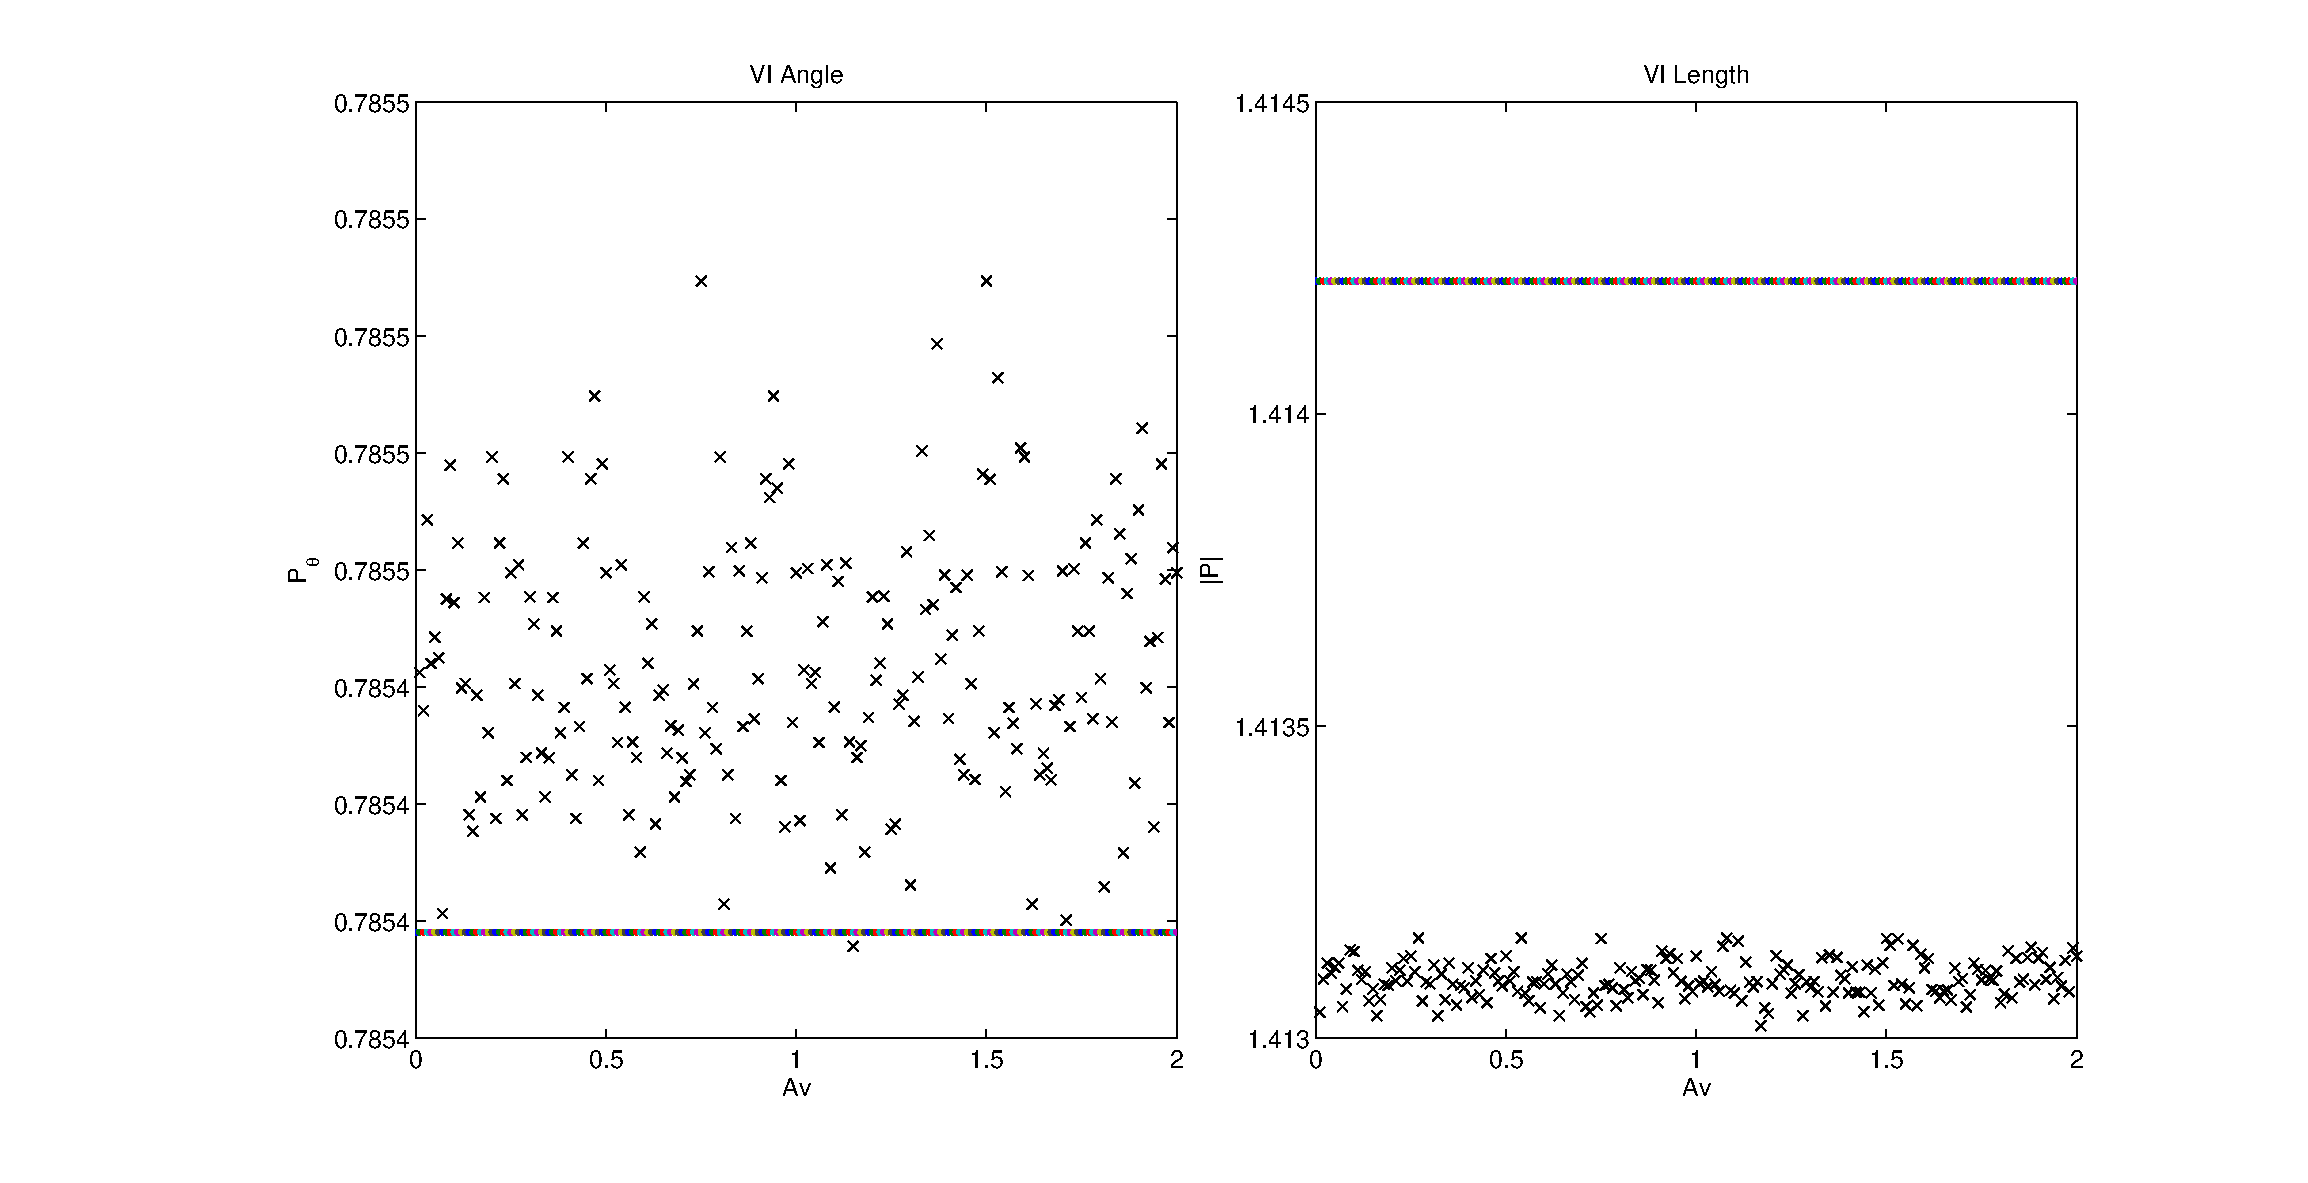
\includegraphics[scale=0.5]{RLcirc_varyV_amp.eps} \\
(b) $P_\theta$ and $|P|$ \\[6pt]
\end{tabular}
\caption{Changing $A_v$.}
\label{fig:Av}
\end{figure}

\subsection{Changing $f_v$}
Consider evaluating the CCM correlations $C_{VI}$ and $C_{IV}$ for each $f_v\in[0.01,2.0]$ in steps of $0.01$.  For reference, both V(t) and I(t) are plotted for different $f_v$ in Figure \ref{fig:fvref}.
\begin{figure}[H]
%\includegraphics{}
\caption{Reference plots for changing $f_v$.}
\label{fig:fvref}
\end{figure}

The CCM correlations are each plotted in Figure \ref{fig:fv} along with the corresponding PAI elements $P_\theta$ and $|P|$.
\begin{figure}[H]
\begin{tabular}{cc}
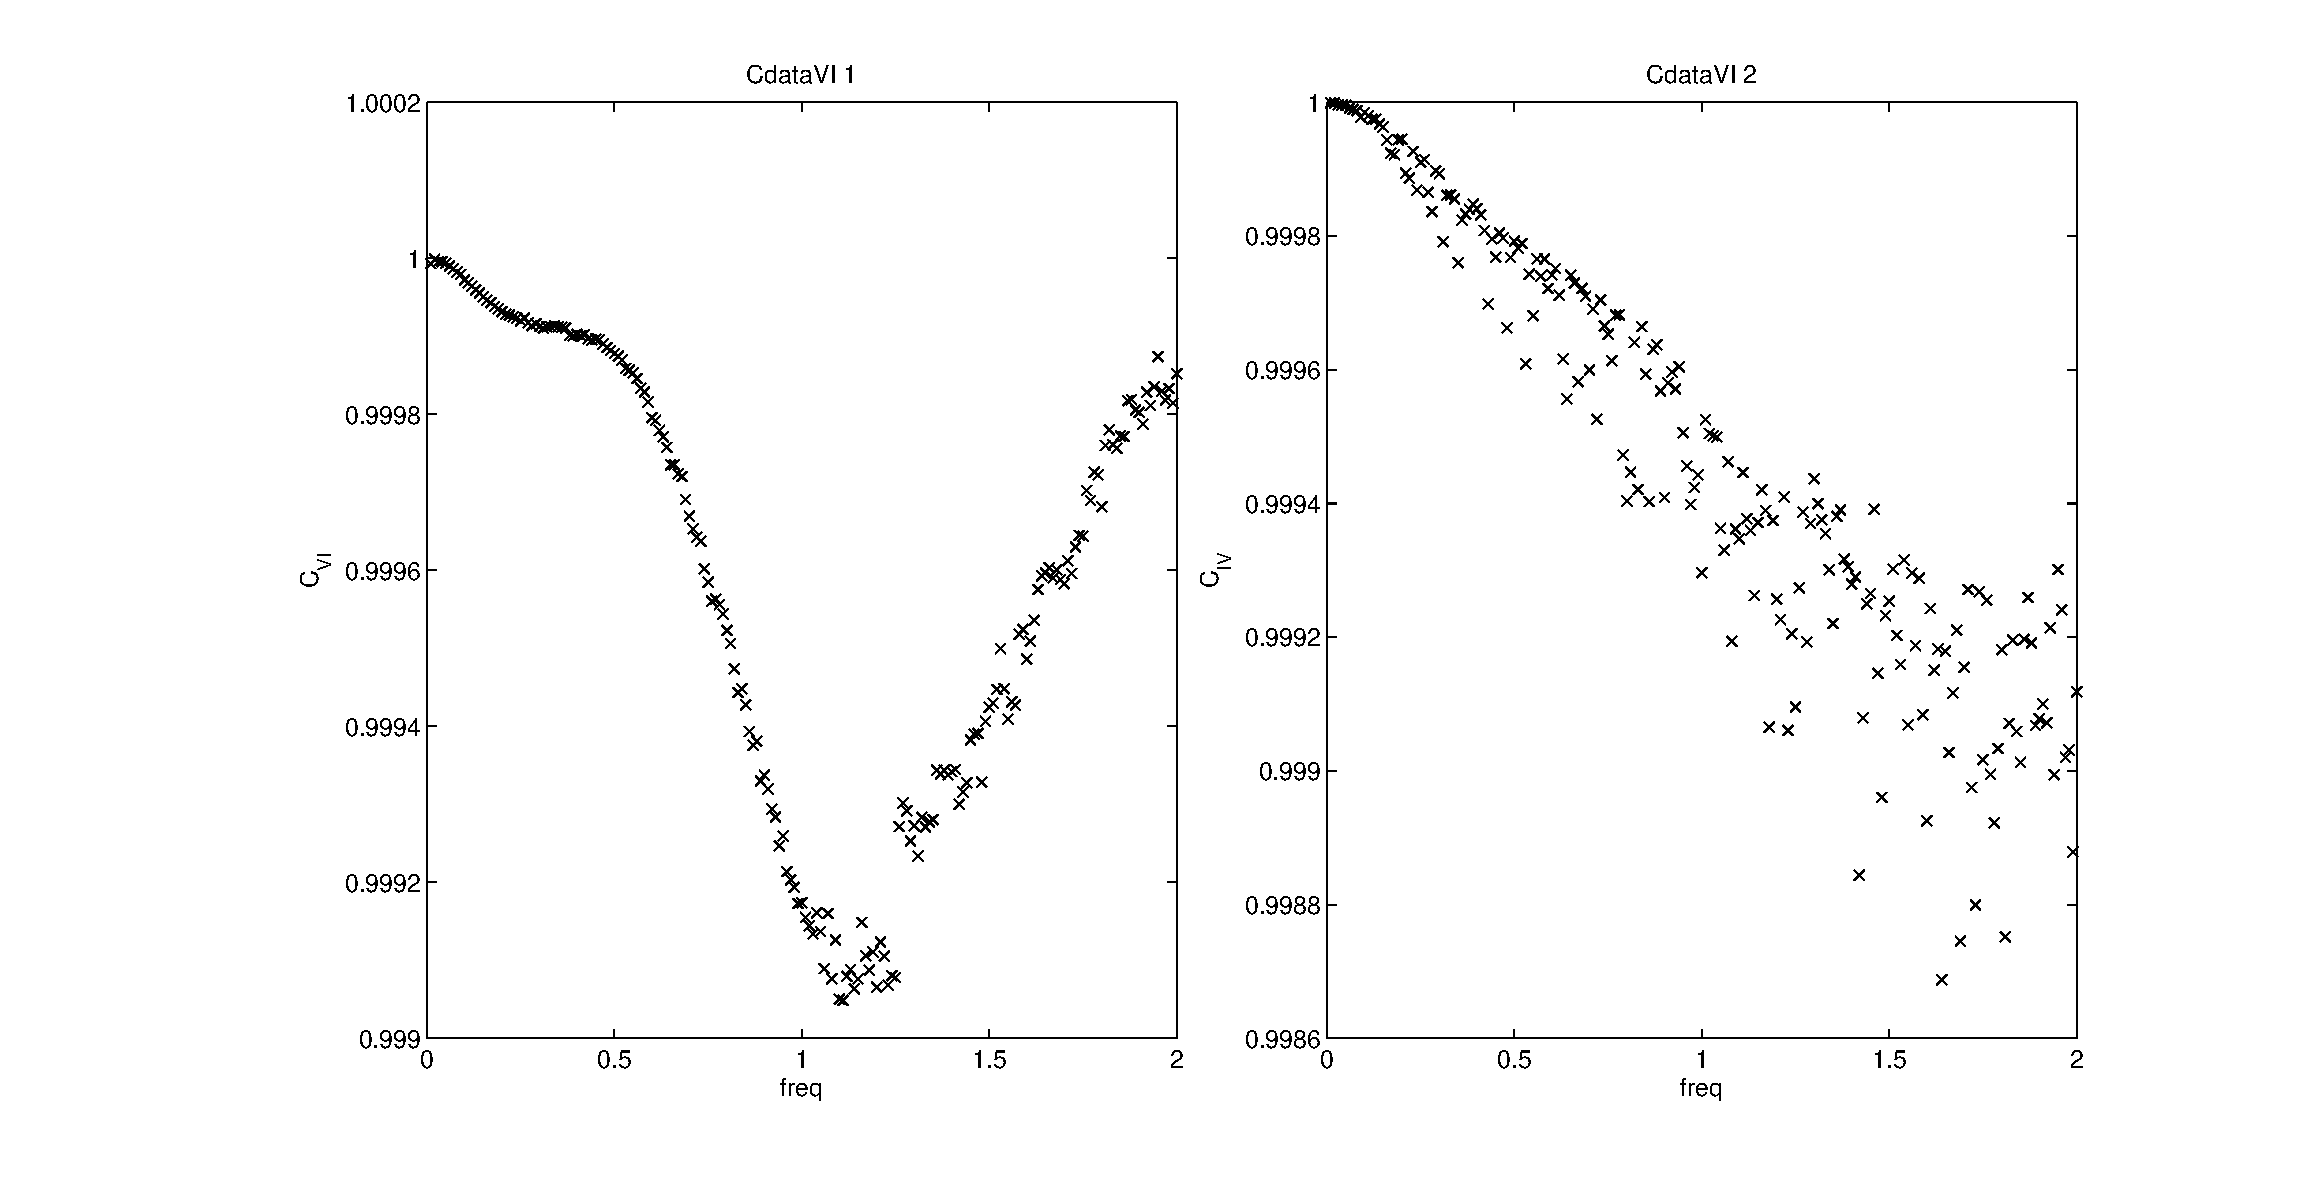
\includegraphics[scale=0.5]{RLcirc_varyV_freq2.eps} \\
(a) $C_{VI}$ and $C_{IV}$ \\[6pt]
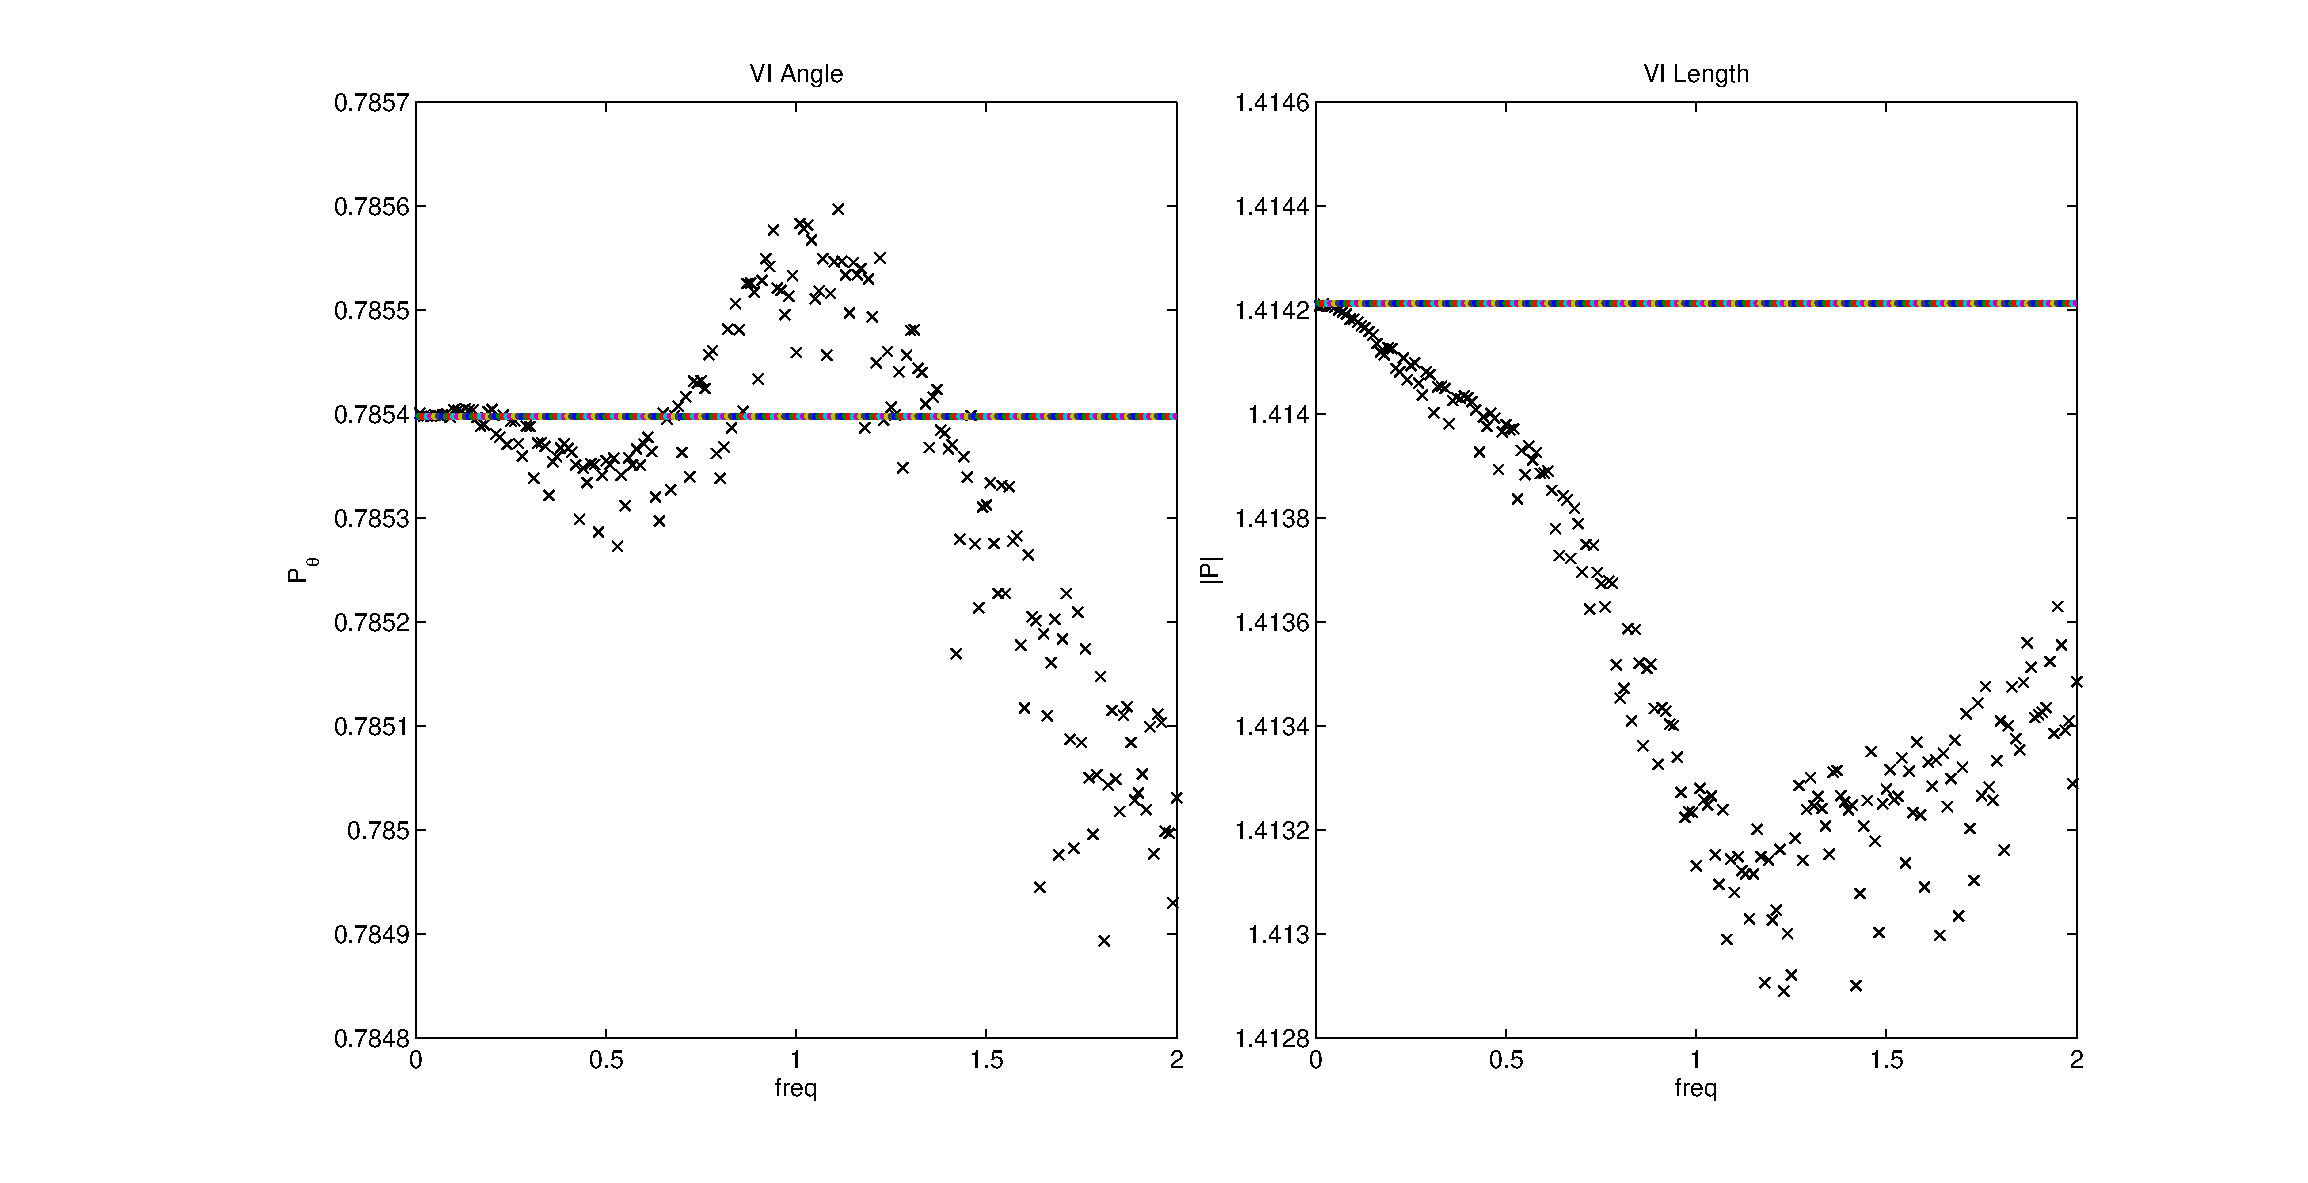
\includegraphics[scale=0.5]{RLcirc_varyV_freq.eps} \\
(b) $P_\theta$ and $|P|$ \\[6pt]
\end{tabular}
\caption{Changing $f_v$.}
\label{fig:fv}
\end{figure}

\subsection{Changing $\phi_v$}
Consider evaluating the CCM correlations $C_{VI}$ and $C_{IV}$ for each $\phi_v\in[0.01,2.0]$ in steps of $0.01$.  For reference, both V(t) and I(t) are plotted for different $\phi_v$ in Figure \ref{fig:Pvref}.
\begin{figure}[H]
%\includegraphics{}
\caption{Reference plots for changing $\phi_v$.}
\label{fig:Pvref}
\end{figure}

The CCM correlations are each plotted in Figure \ref{fig:Pv} along with the corresponding PAI elements $P_\theta$ and $|P|$.
\begin{figure}[H]
\begin{tabular}{cc}
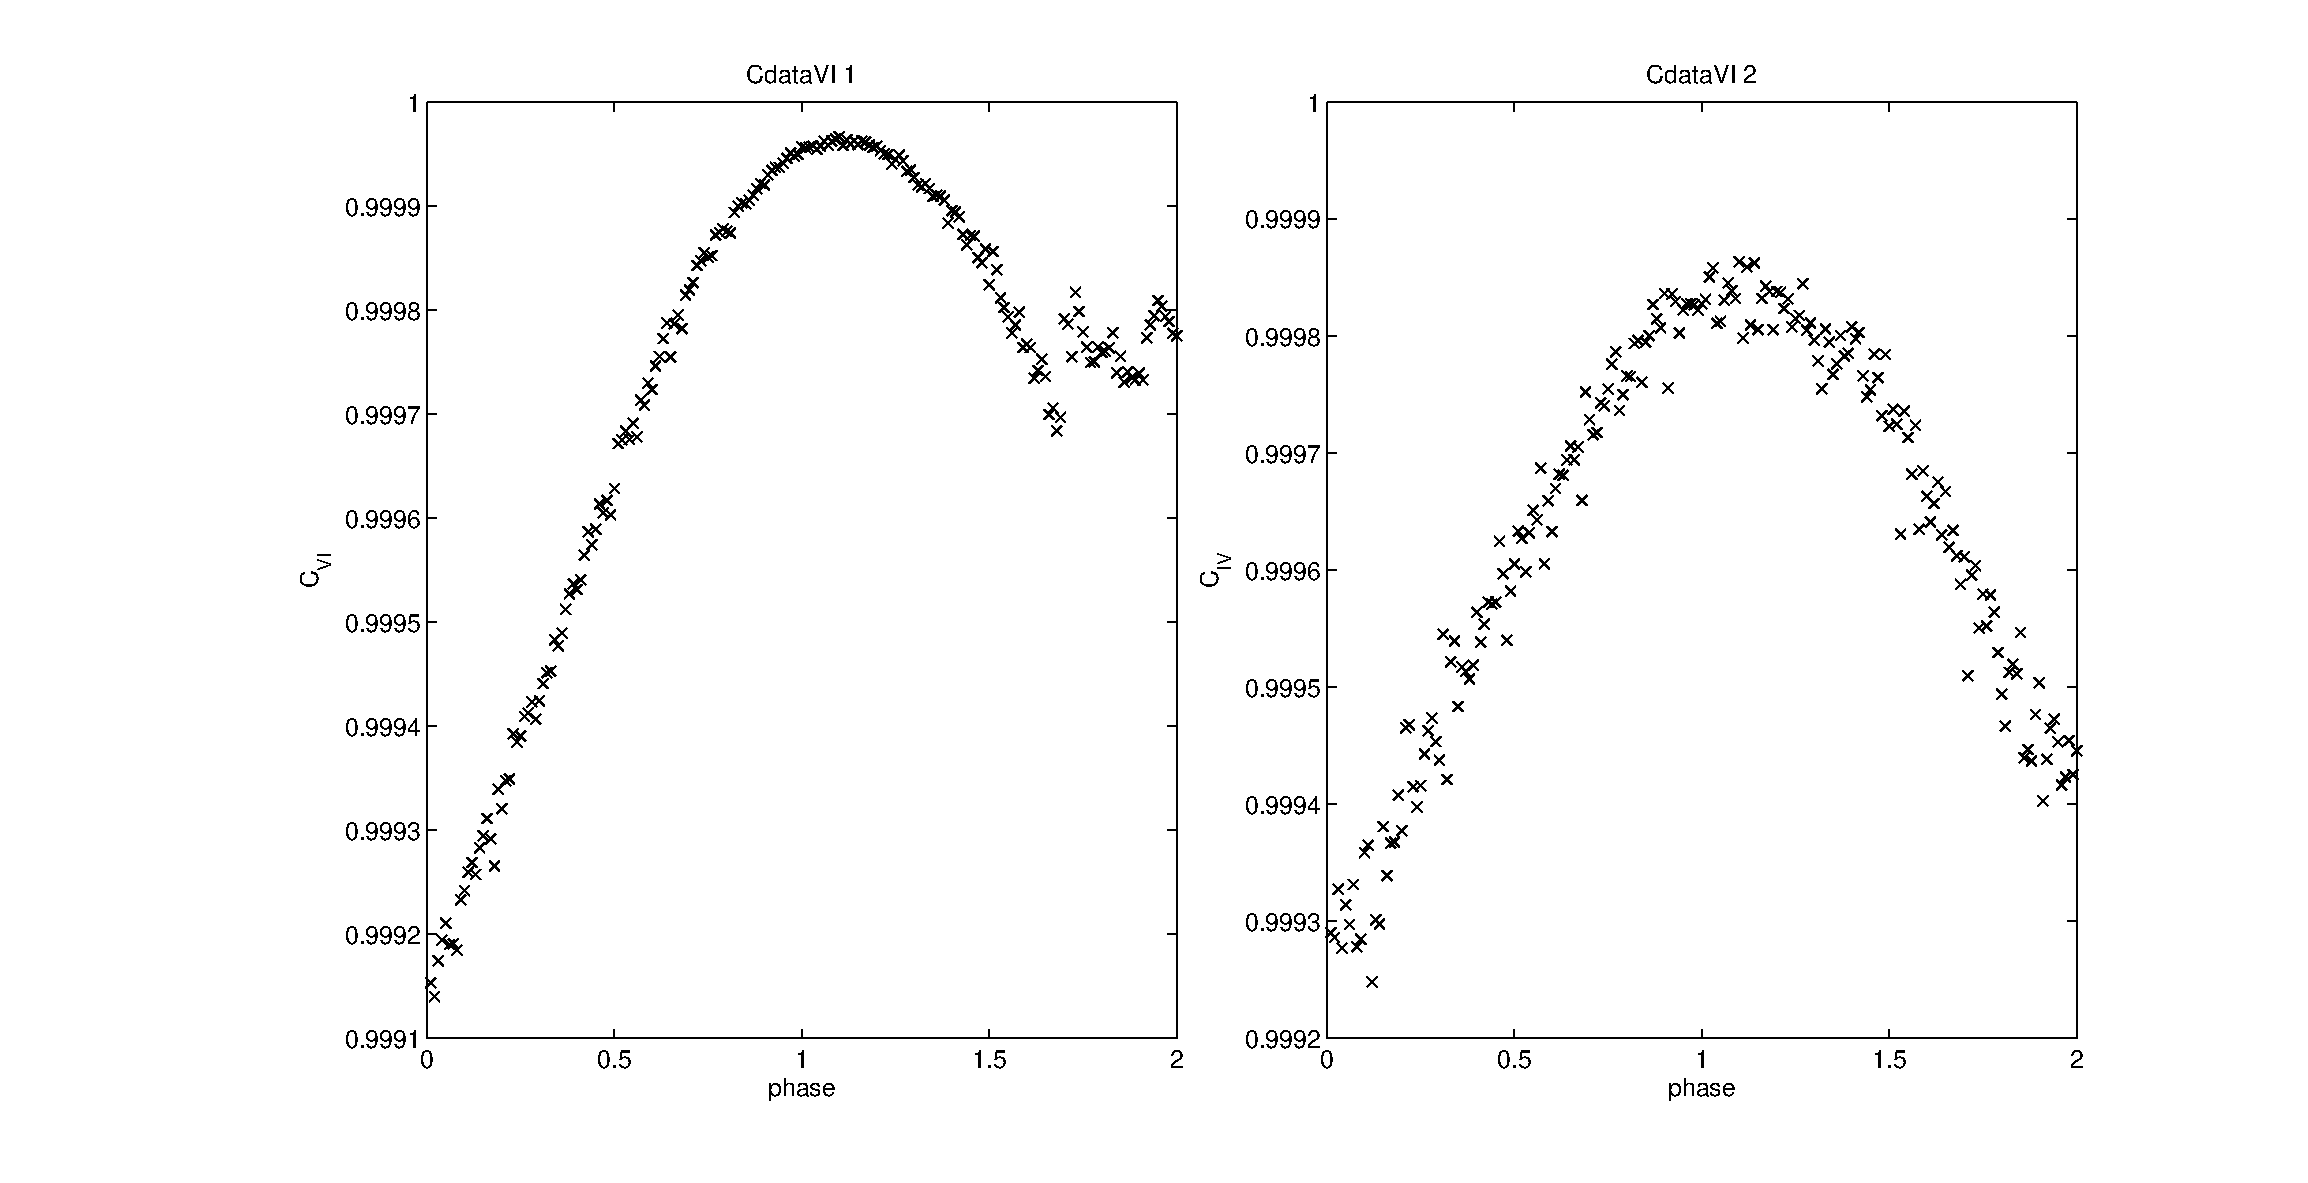
\includegraphics[scale=0.5]{RLcirc_varyV_phase2.eps} \\
(a) $C_{VI}$ and $C_{IV}$ \\[6pt]
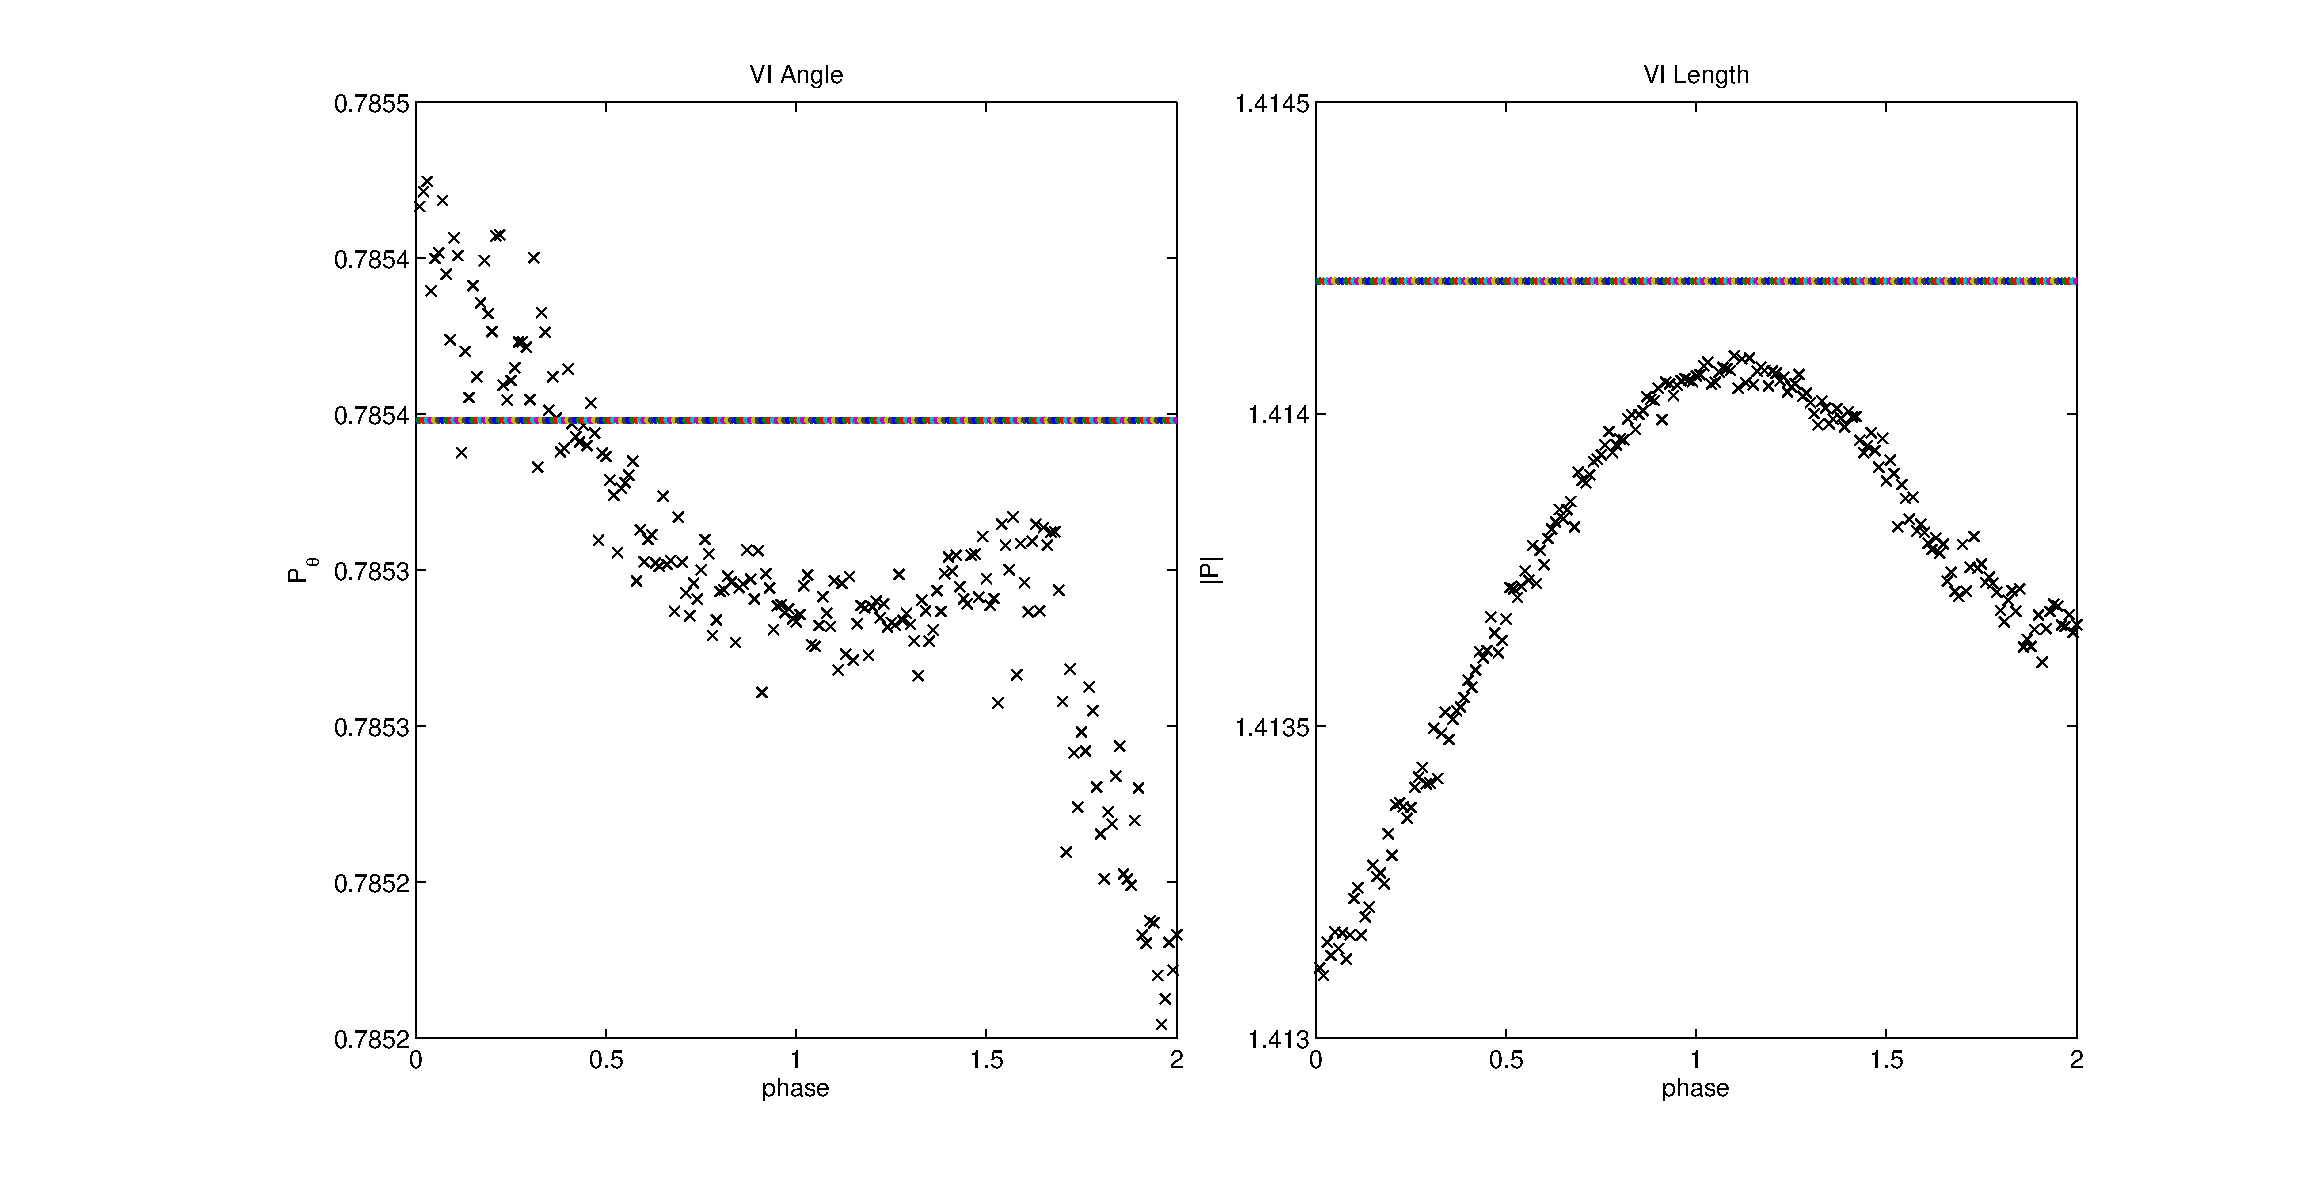
\includegraphics[scale=0.5]{RLcirc_varyV_phase.eps} \\
(b) $P_\theta$ and $|P|$ \\[6pt]
\end{tabular}
\caption{Changing $\phi_v$.}
\label{fig:Pv}
\end{figure}

\subsection{Changing $O_v$}
Consider evaluating the CCM correlations $C_{VI}$ and $C_{IV}$ for each $O_v\in[0.01,2.0]$ in steps of $0.01$.  For reference, both V(t) and I(t) are plotted for different $O_v$ in Figure \ref{fig:Ovref}.
\begin{figure}[H]
%\includegraphics{}
\caption{Reference plots for changing $O_v$.}
\label{fig:Ovref}
\end{figure}

The CCM correlations are each plotted in Figure \ref{fig:Ov} along with the corresponding PAI elements $P_\theta$ and $|P|$.
\begin{figure}[H]
\begin{tabular}{cc}
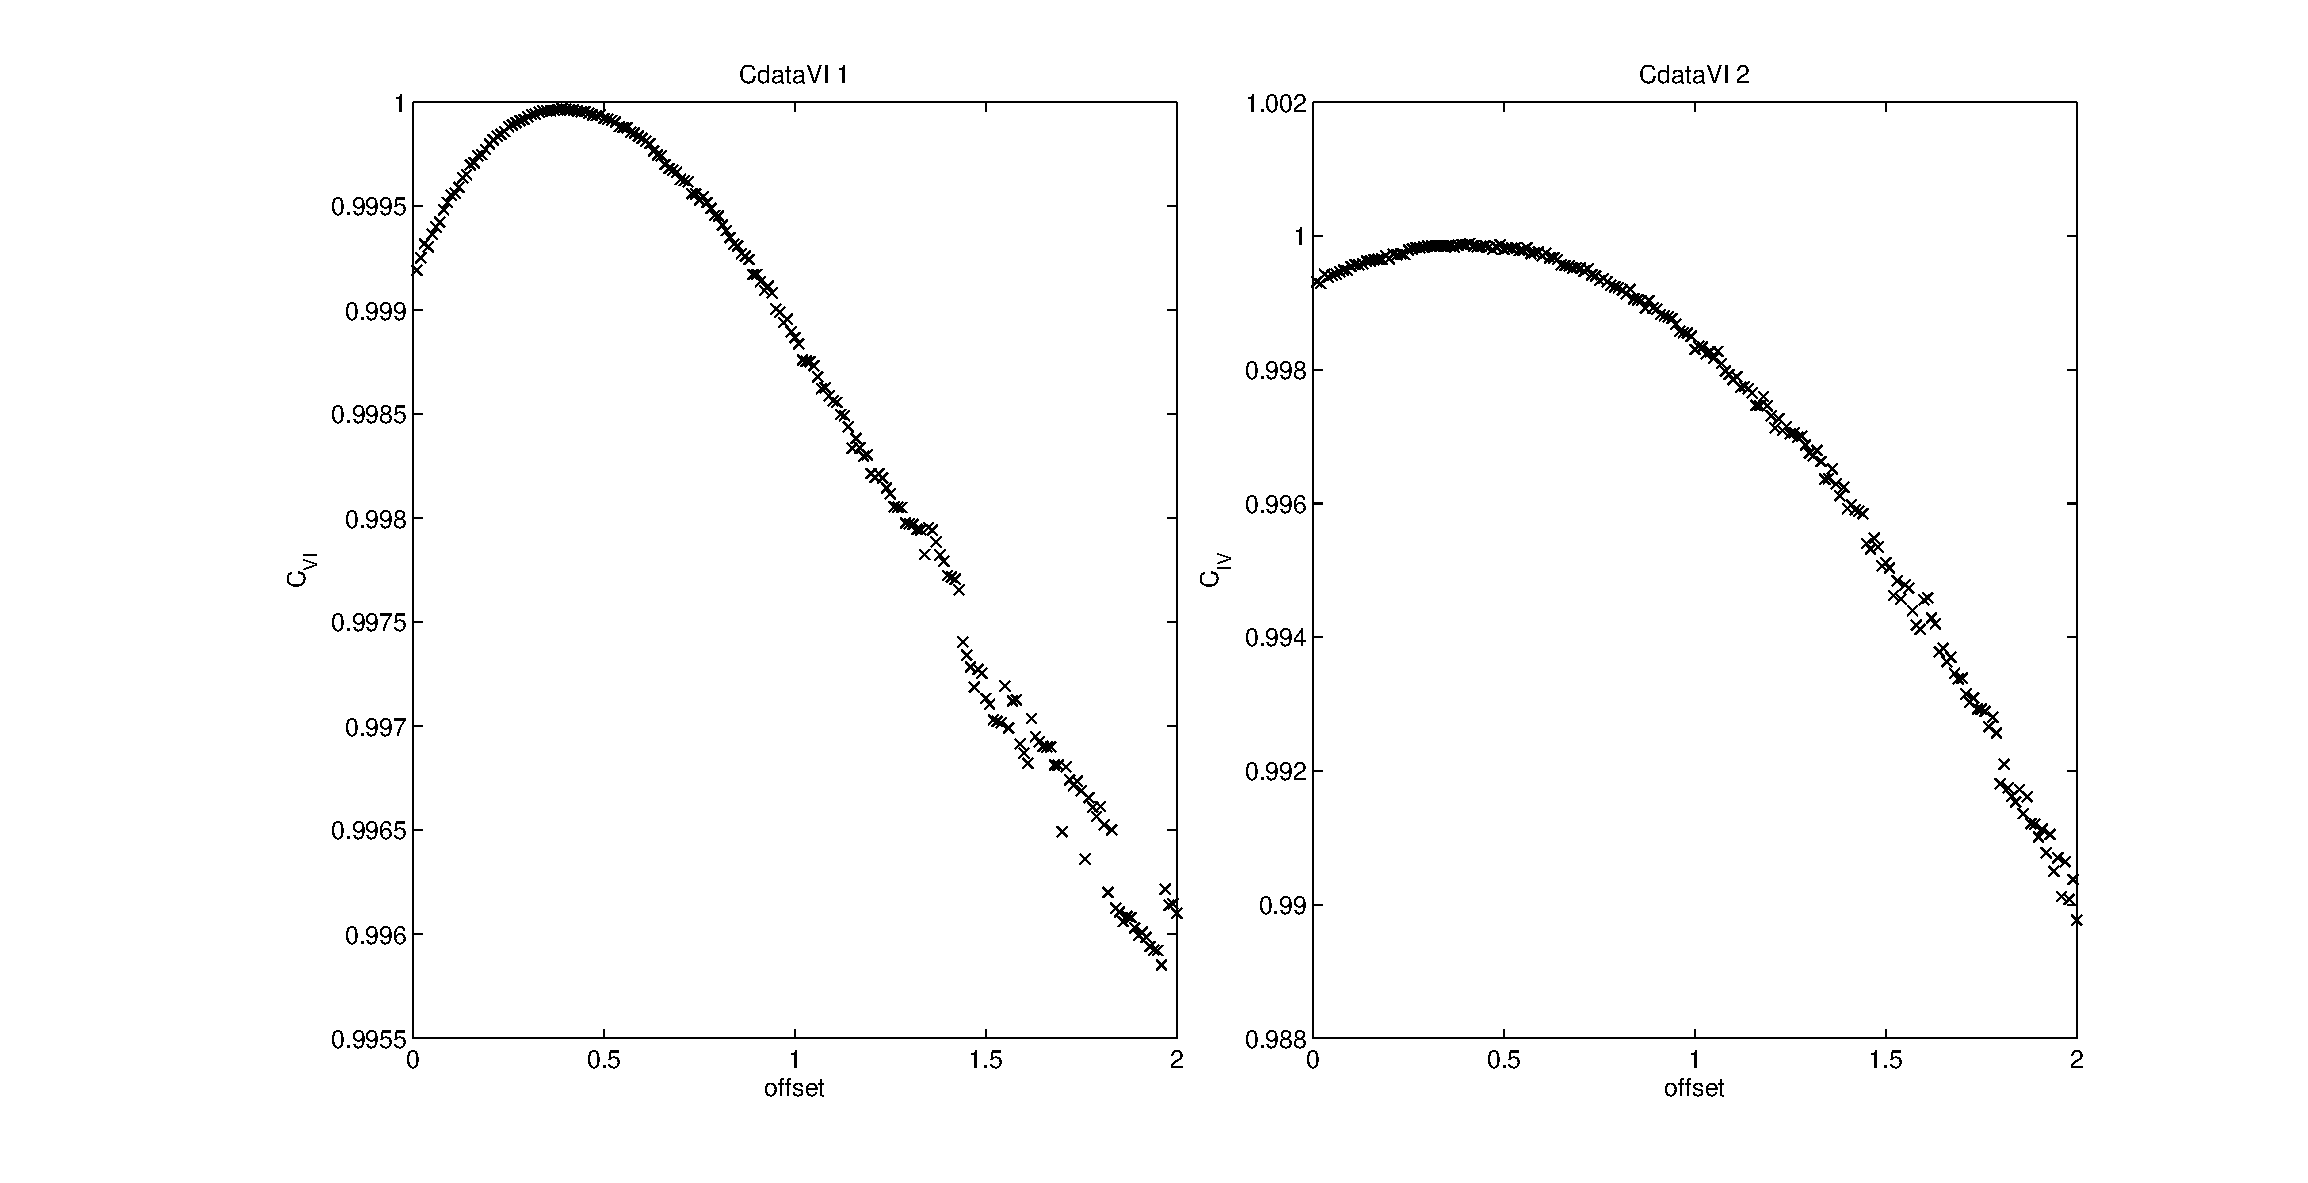
\includegraphics[scale=0.5]{RLcirc_varyV_offset2.eps} \\
(a) $C_{VI}$ and $C_{IV}$ \\[6pt]
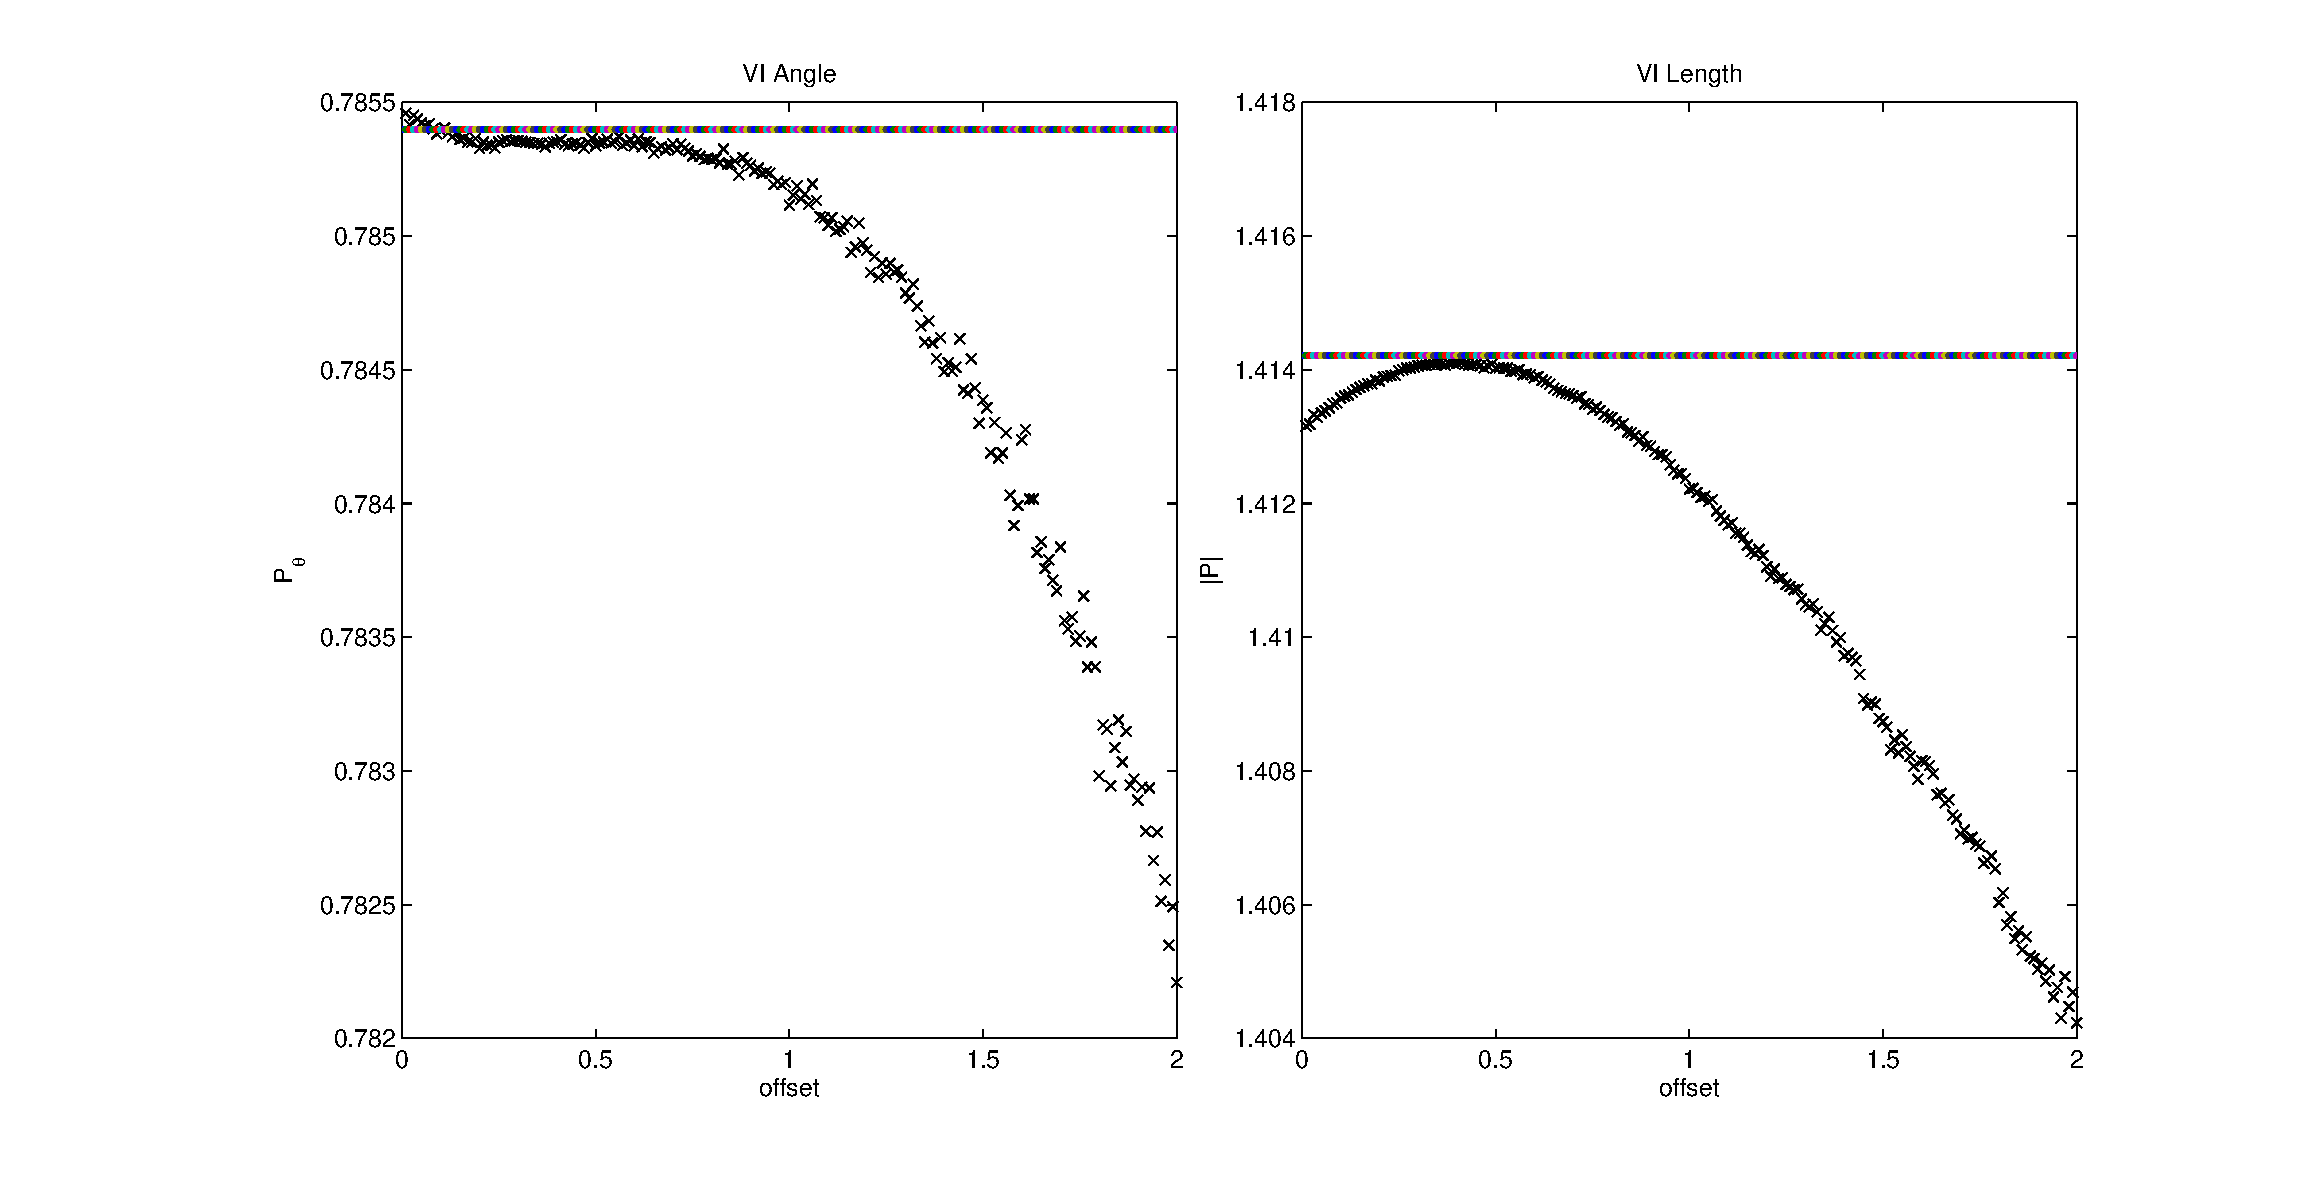
\includegraphics[scale=0.5]{RLcirc_varyV_offset.eps} \\
(b) $P_\theta$ and $|P|$ \\[6pt]
\end{tabular}
\caption{Changing $O_v$.}
\label{fig:Ov}
\end{figure}

Figure \ref{fig:Ov1} shows the effect of increasing the library length from $2\times10^3$ (i.e.\ {\tt tspan = [0:0.5:1000];}) to $10^4$ (i.e.\ {\tt tspan = [0:0.5:5000];}), and Figure \ref{fig:Ov2} extends the above plots to $O_v\in[0.01,10.0]$ in steps of $0.05$.
\begin{figure}[H]
\begin{tabular}{cc}
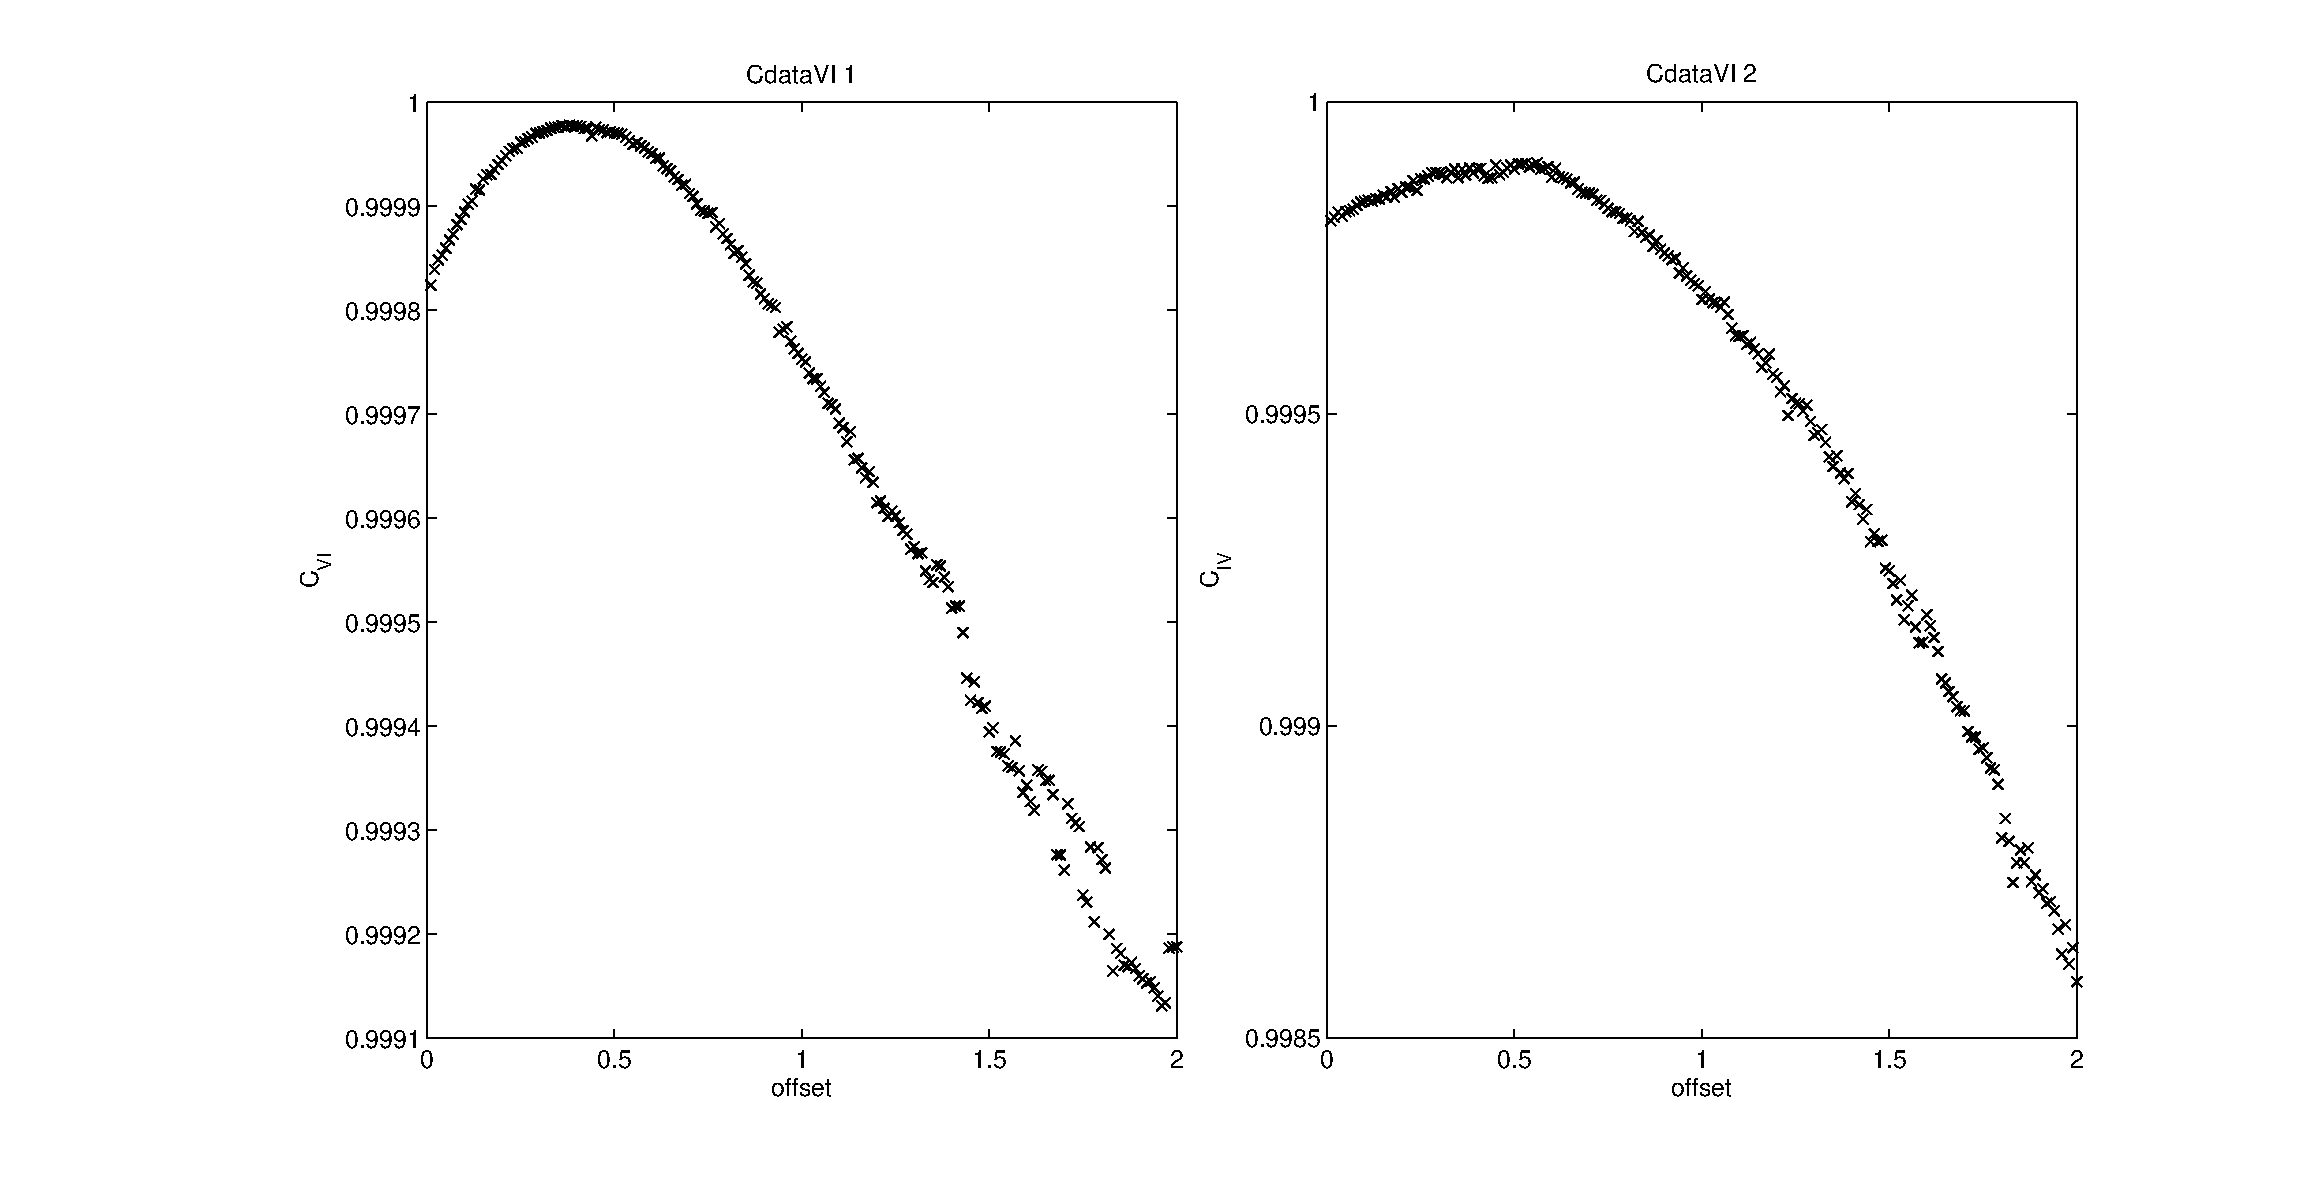
\includegraphics[scale=0.5]{RLcirc_varyV_offsetLup2.eps} \\
(a) $C_{VI}$ and $C_{IV}$ \\[6pt]
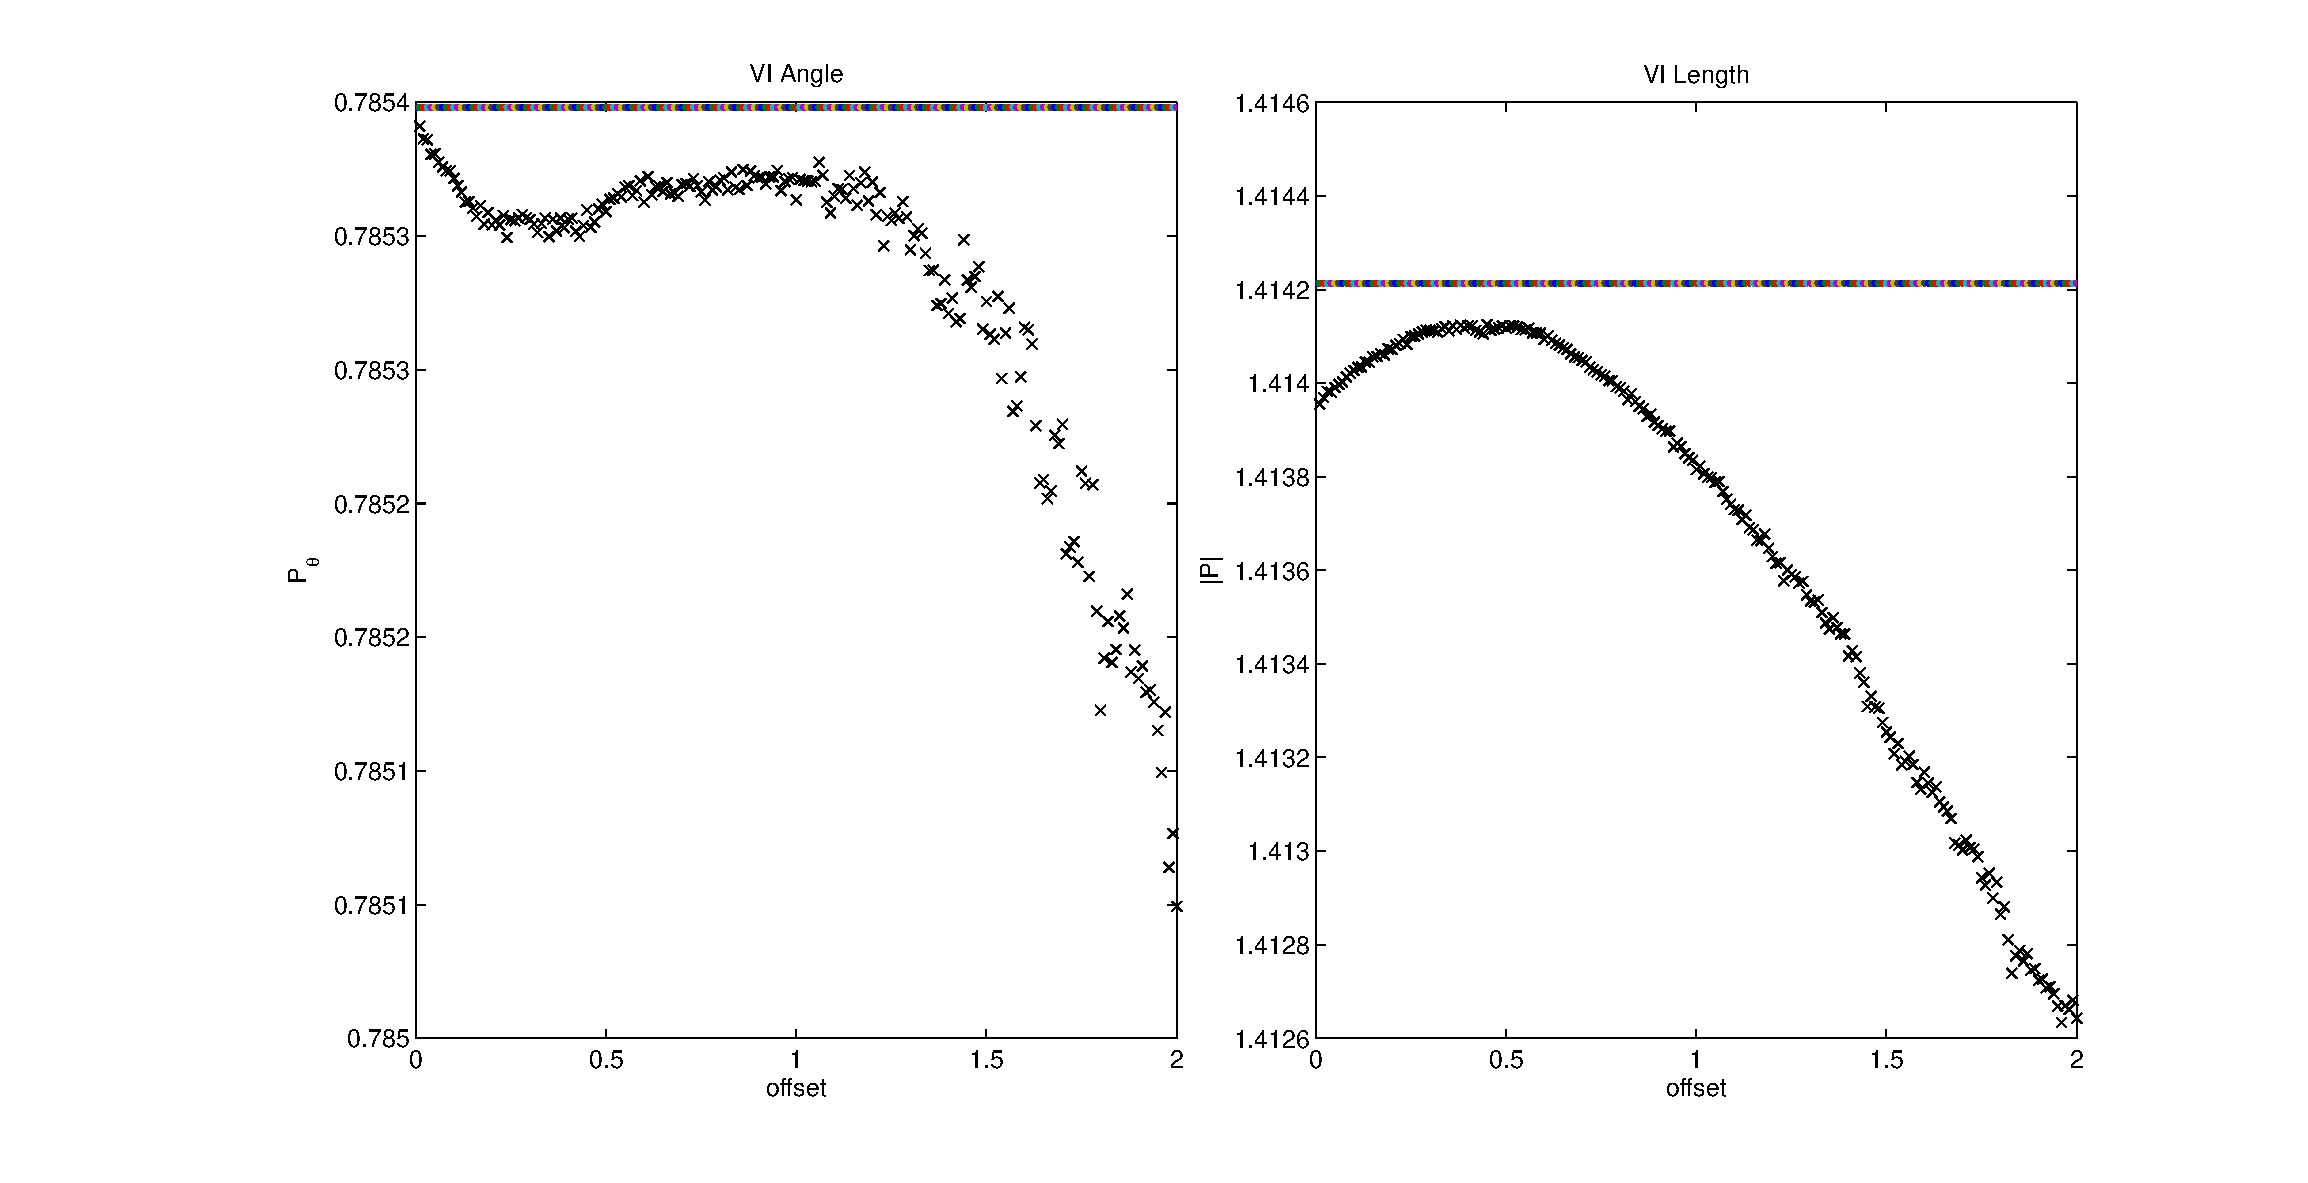
\includegraphics[scale=0.5]{RLcirc_varyV_offsetLup.eps} \\
(b) $P_\theta$ and $|P|$ \\[6pt]
\end{tabular}
\caption{Changing $O_v$ (longer library length).}
\label{fig:Ov1}
\end{figure}
\begin{figure}[H]
\begin{tabular}{cc}
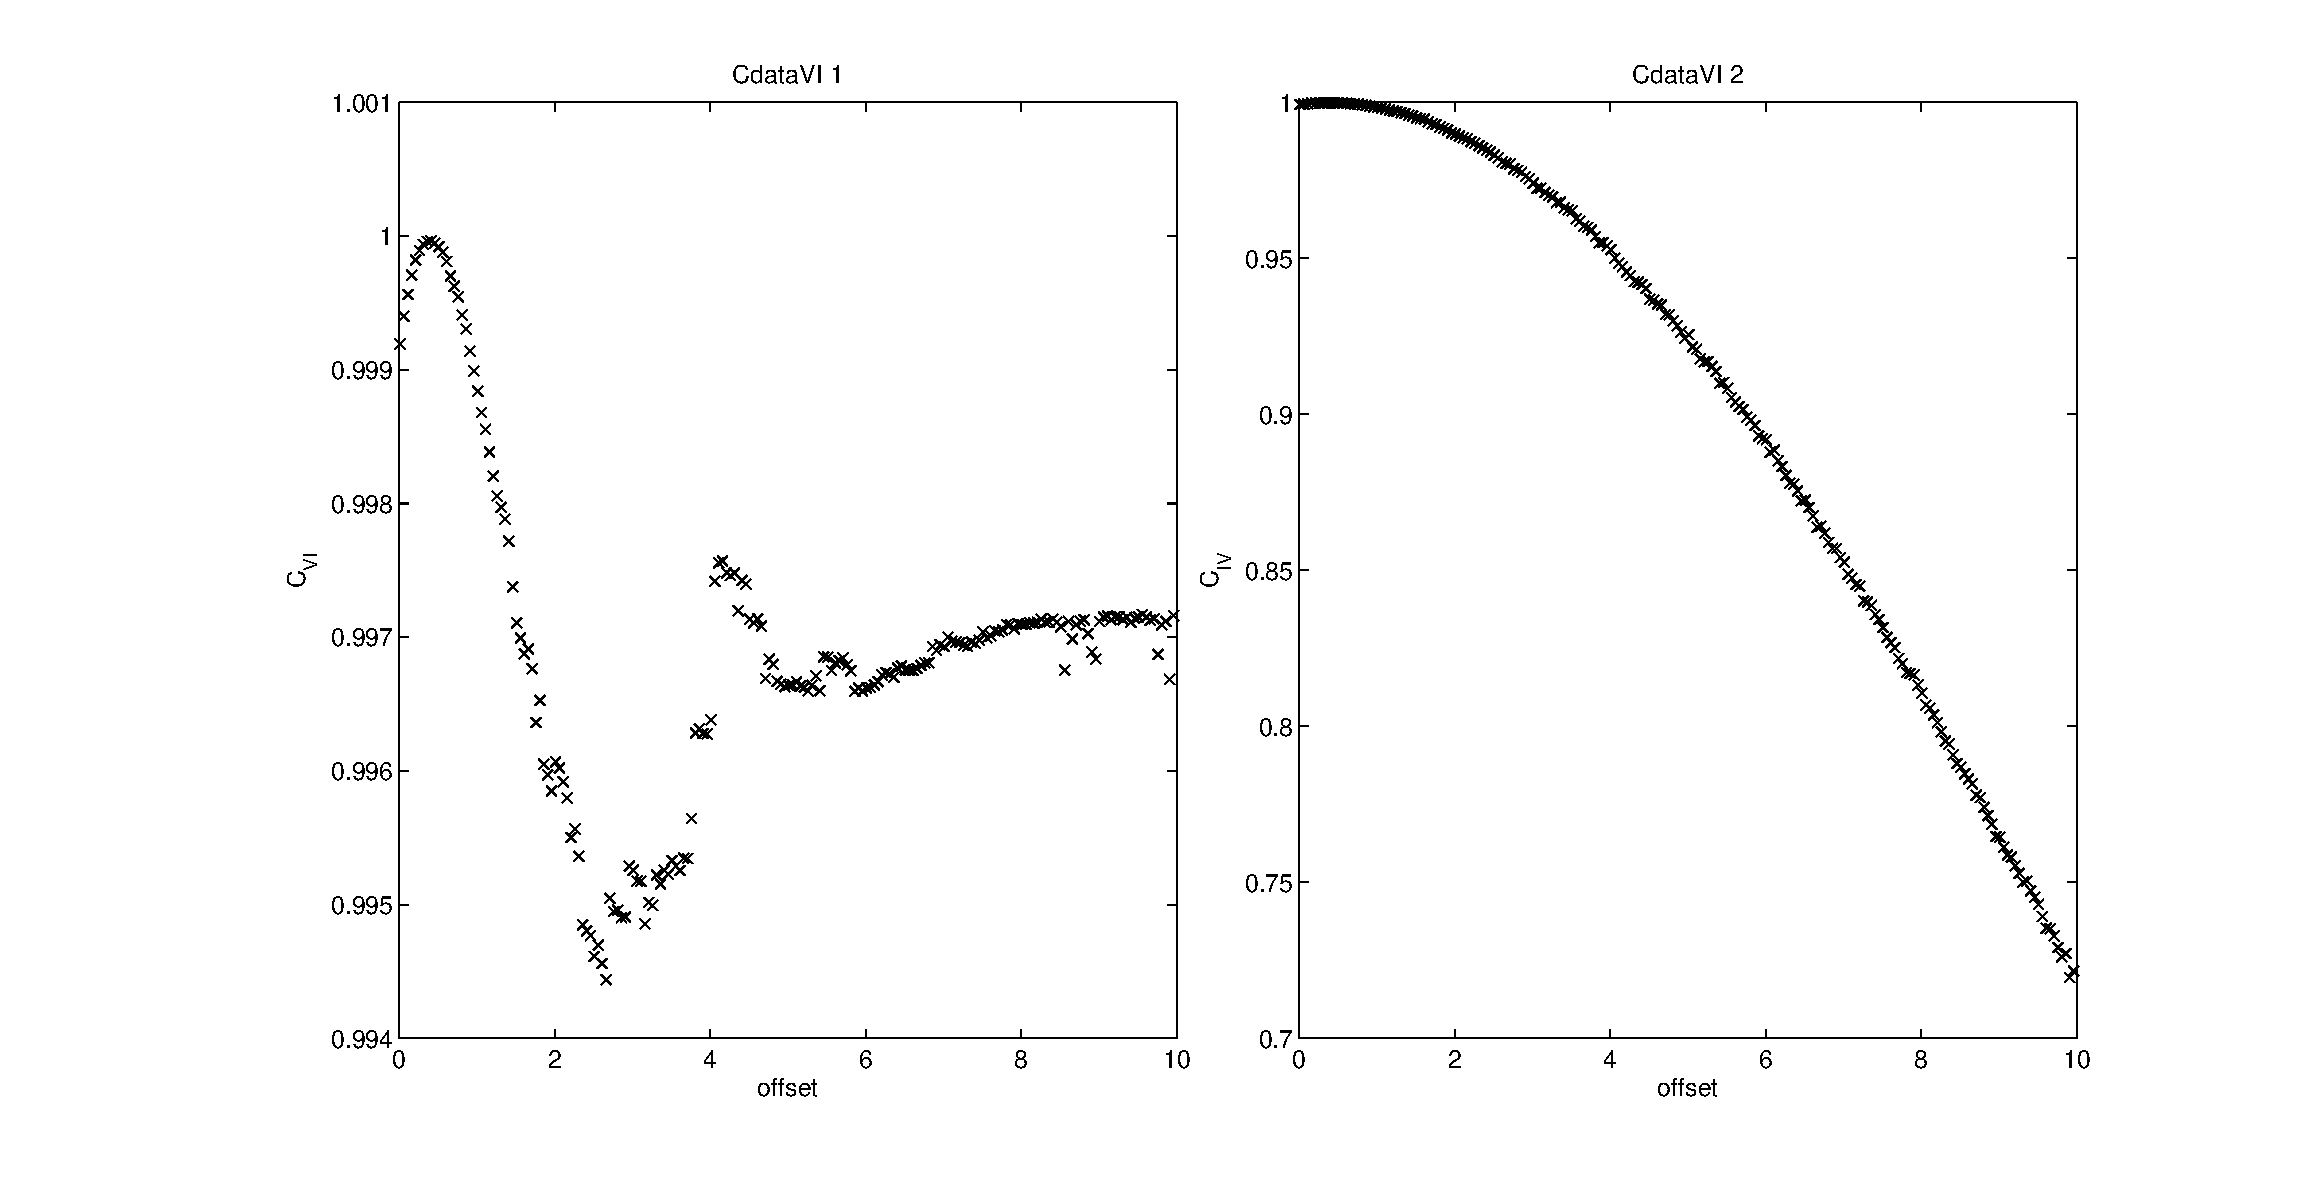
\includegraphics[scale=0.5]{RLcirc_varyV_offsetlong2.eps} \\
(a) $C_{VI}$ and $C_{IV}$ \\[6pt]
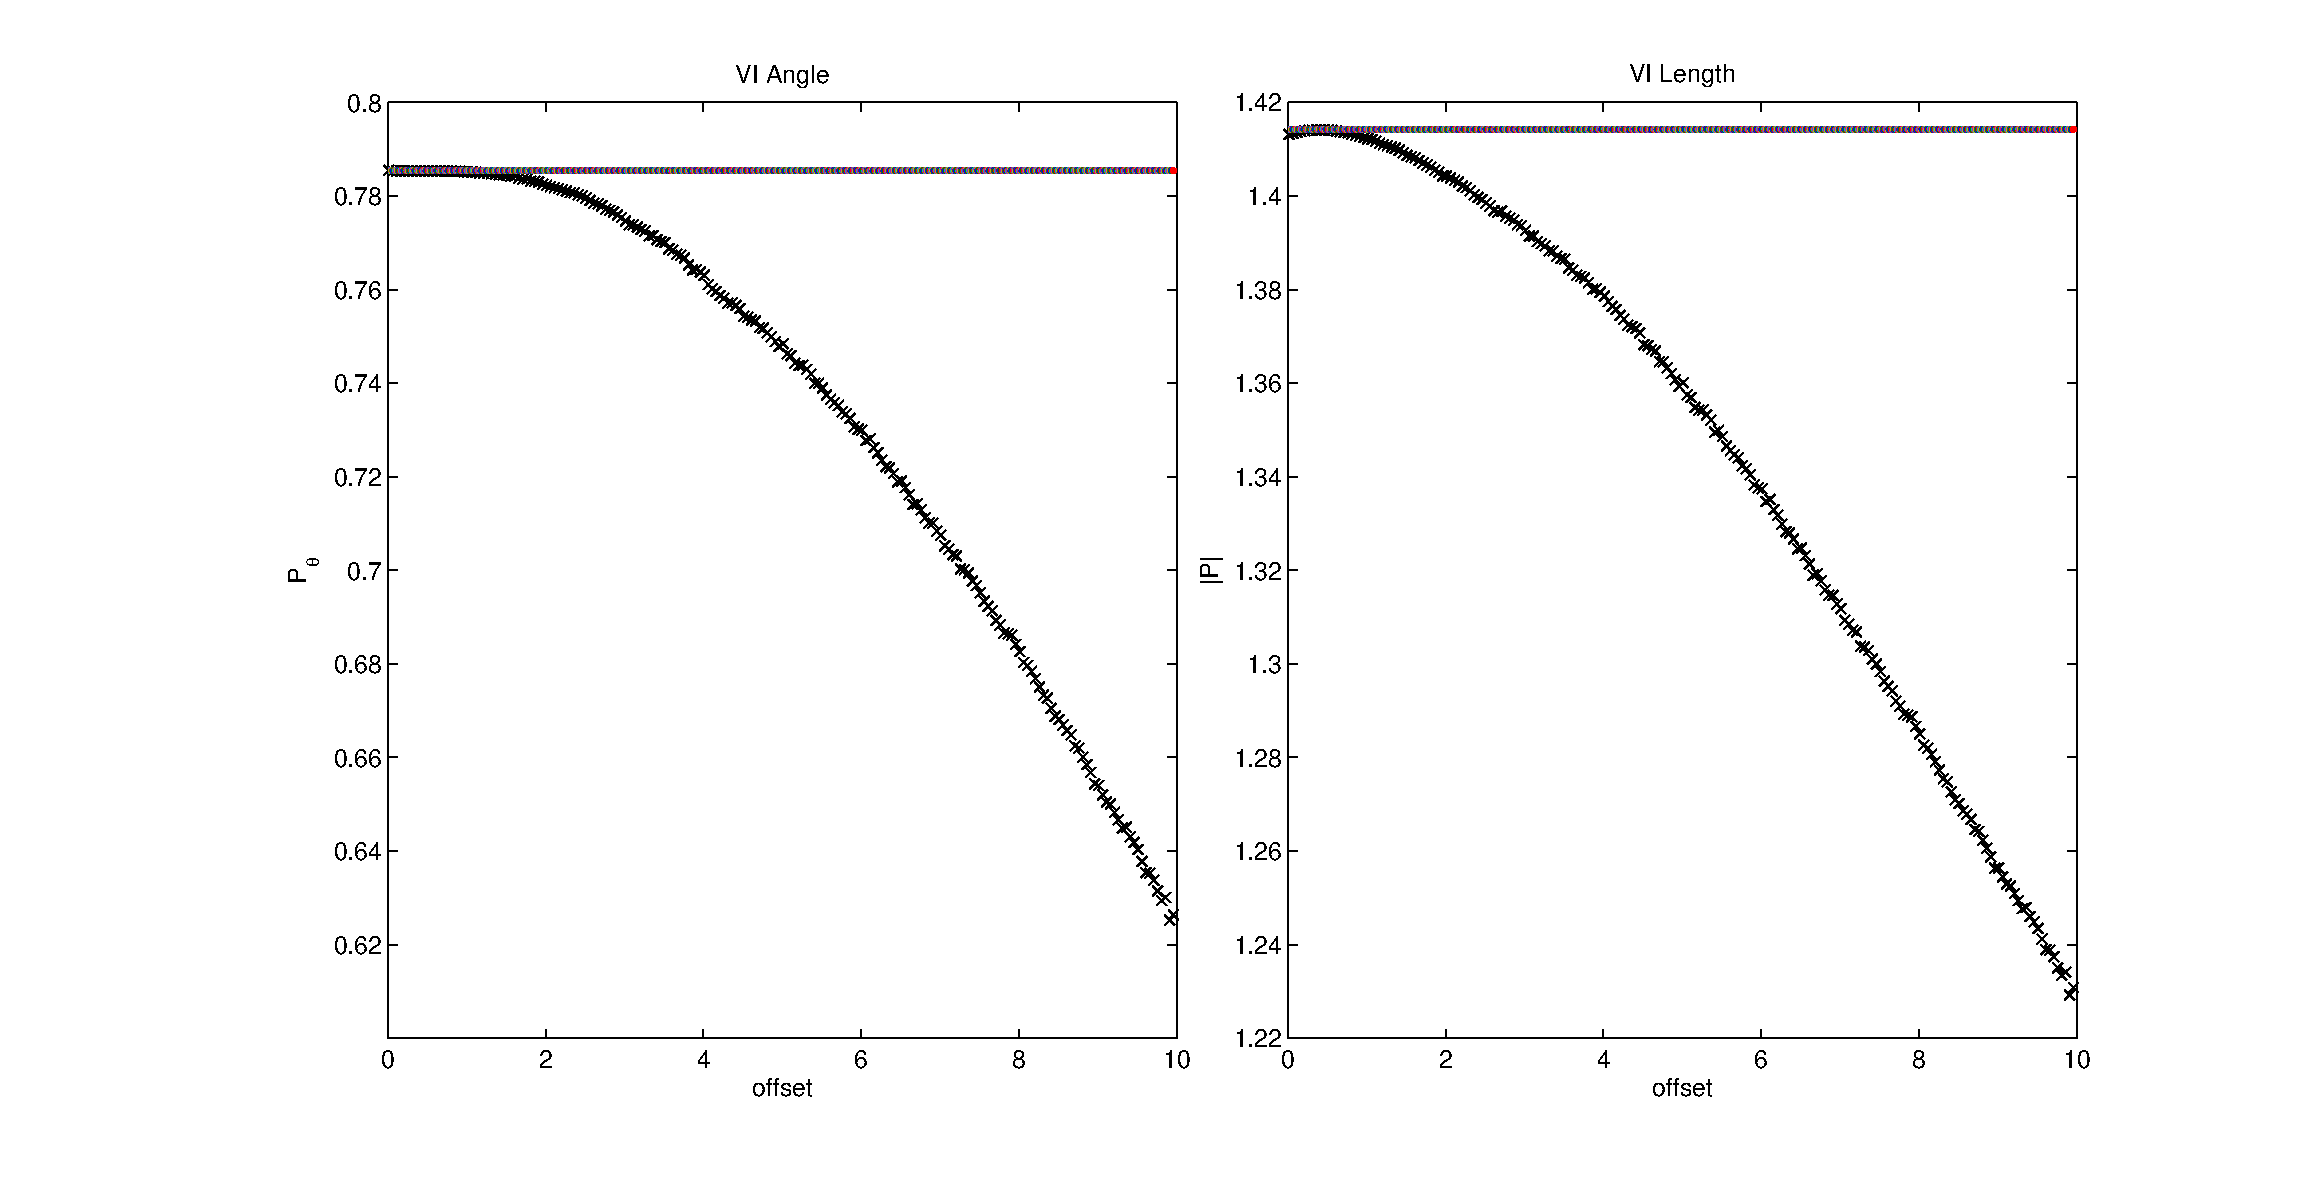
\includegraphics[scale=0.5]{RLcirc_varyV_offsetlong.eps} \\
(c) $P_\theta$ and $|P|$ \\[6pt]
\end{tabular}
\caption{Changing $O_v$ (larger domain for $O_v$).}
\label{fig:Ov2}
\end{figure}

\begin{comment}
\section{Changing R(t)}
Consider the situation where $V(t)$ is constant.
\begin{center}
{\large {\bf Physical intuition is that $R$ drives $I$, so we expect to find $R$ CCM causes $I$ ($C_{RI}>C_{IR}$).}}
\end{center}
For this example, the voltage is described by 
\begin{equation}
R(t) = A_r \sin\left(f_r t+\phi_r\right)+O_r,
\end{equation}
where $A_r$ is the amplitude, $f_r$ is the frequency, $\phi_r$ is the phase, and $O_r$ is the offset voltage.

\subsection{Changing $A_r$}
Consider evaluating the CCM correlations $C_{VI}$ and $C_{IV}$ for each $A_r\in[0.01,2.0]$ in steps of $0.01$.  For reference, both R(t) and I(t) are plotted for different $A_r$ in Figure \ref{fig:Arref}.
\begin{figure}[H]
%\includegraphics{}
\caption{Reference plots for changing $A_r$.}
\label{fig:Arref}
\end{figure}

The CCM correlations are each plotted in Figure \ref{fig:Ar} along with the corresponding PAI elements $P_\theta$ and $|P|$.
\begin{figure}[H]
\begin{tabular}{cc}
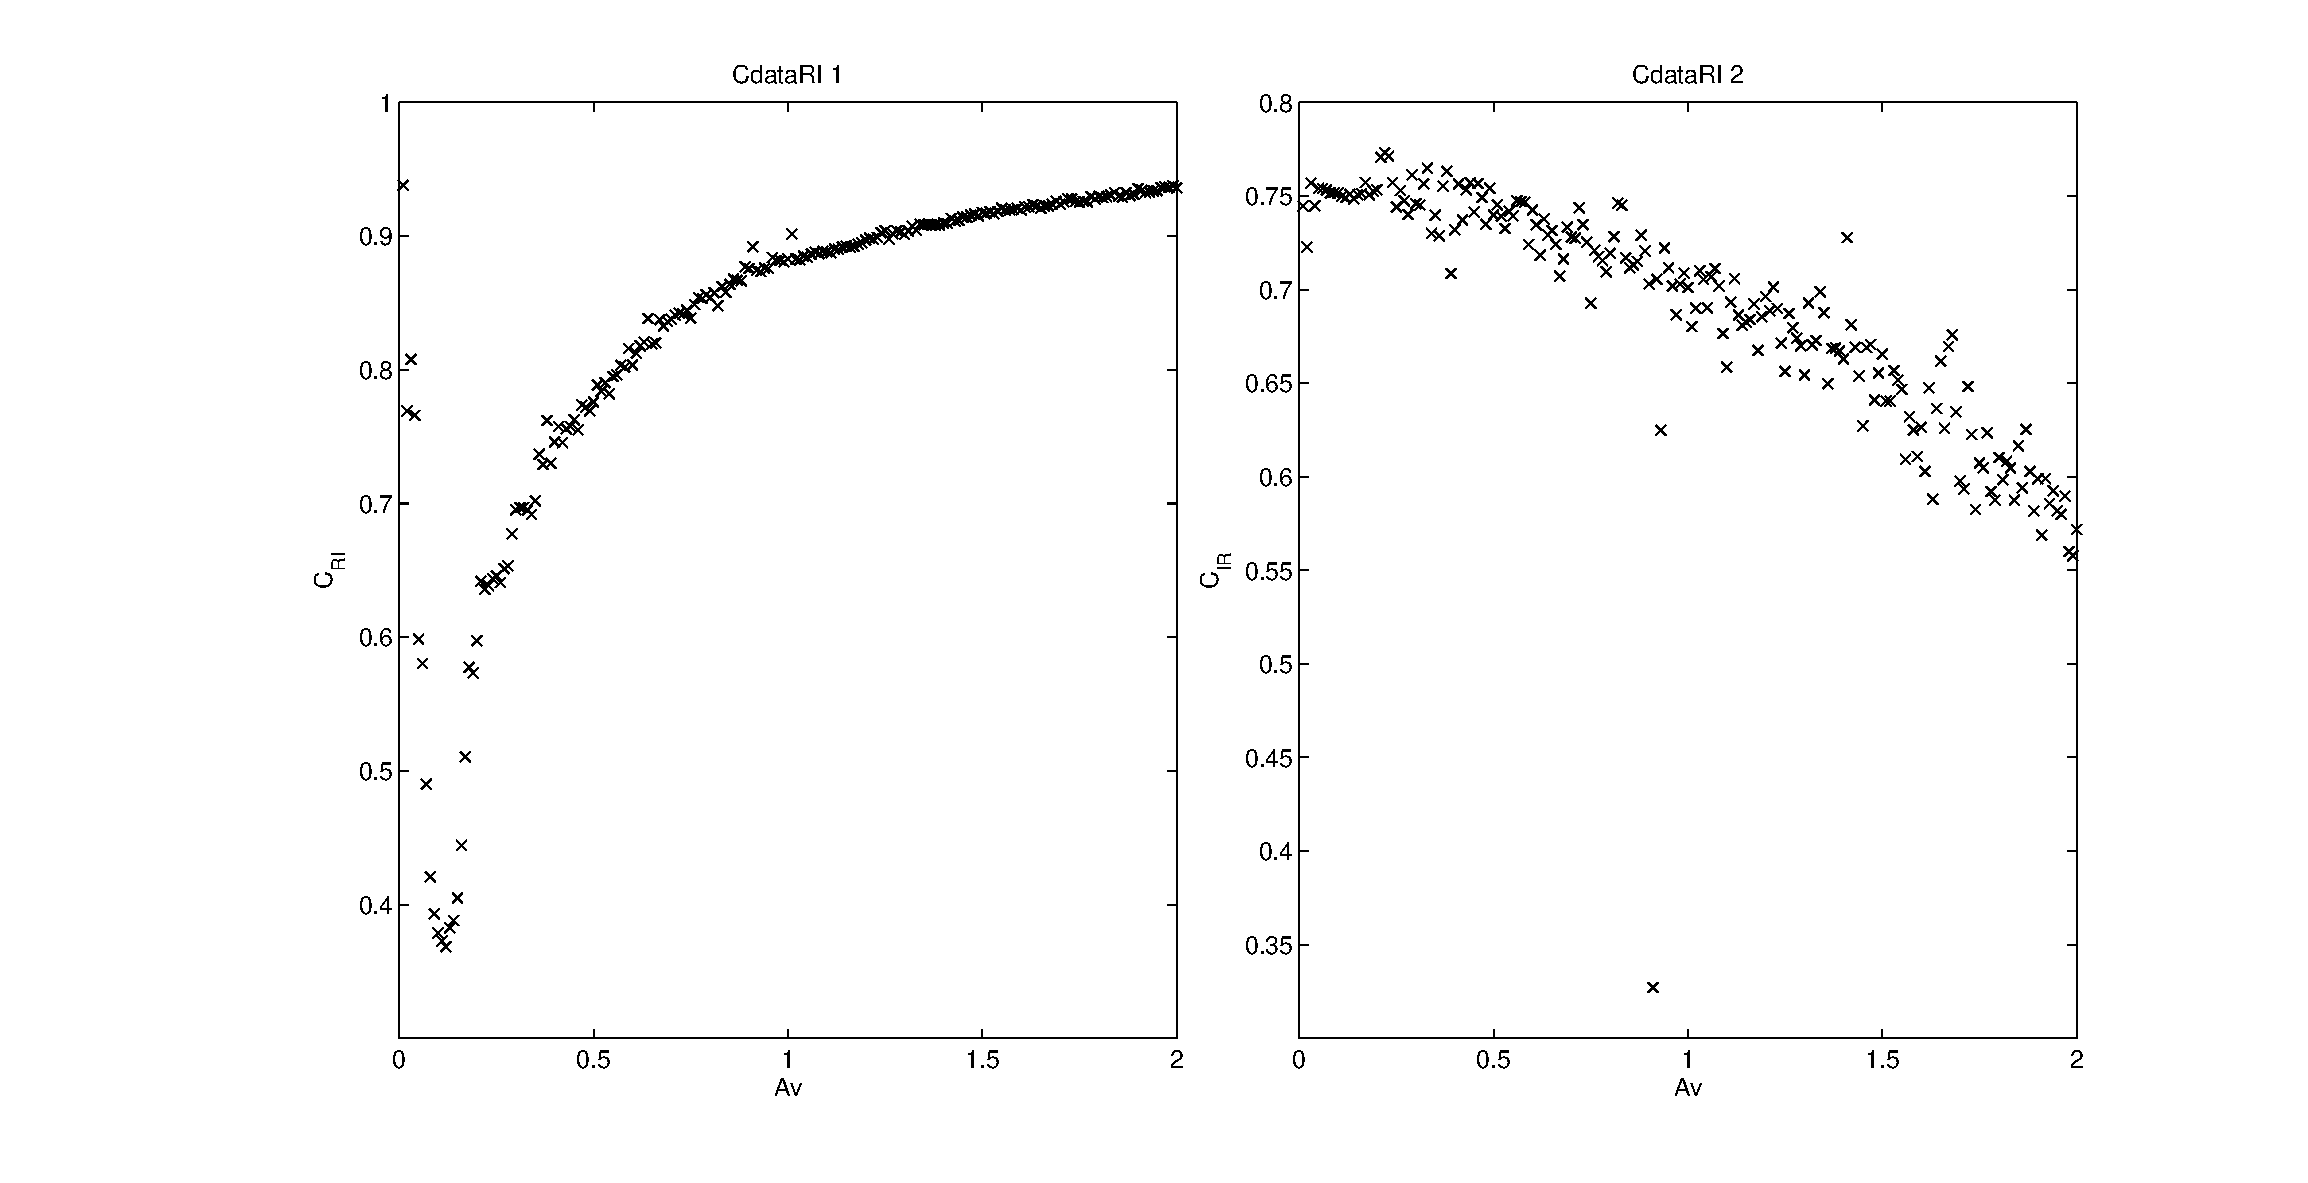
\includegraphics[scale=0.5]{RLcirc_varyR_amp2.eps} \\
(a) $C_{VI}$ and $C_{IV}$ \\[6pt]
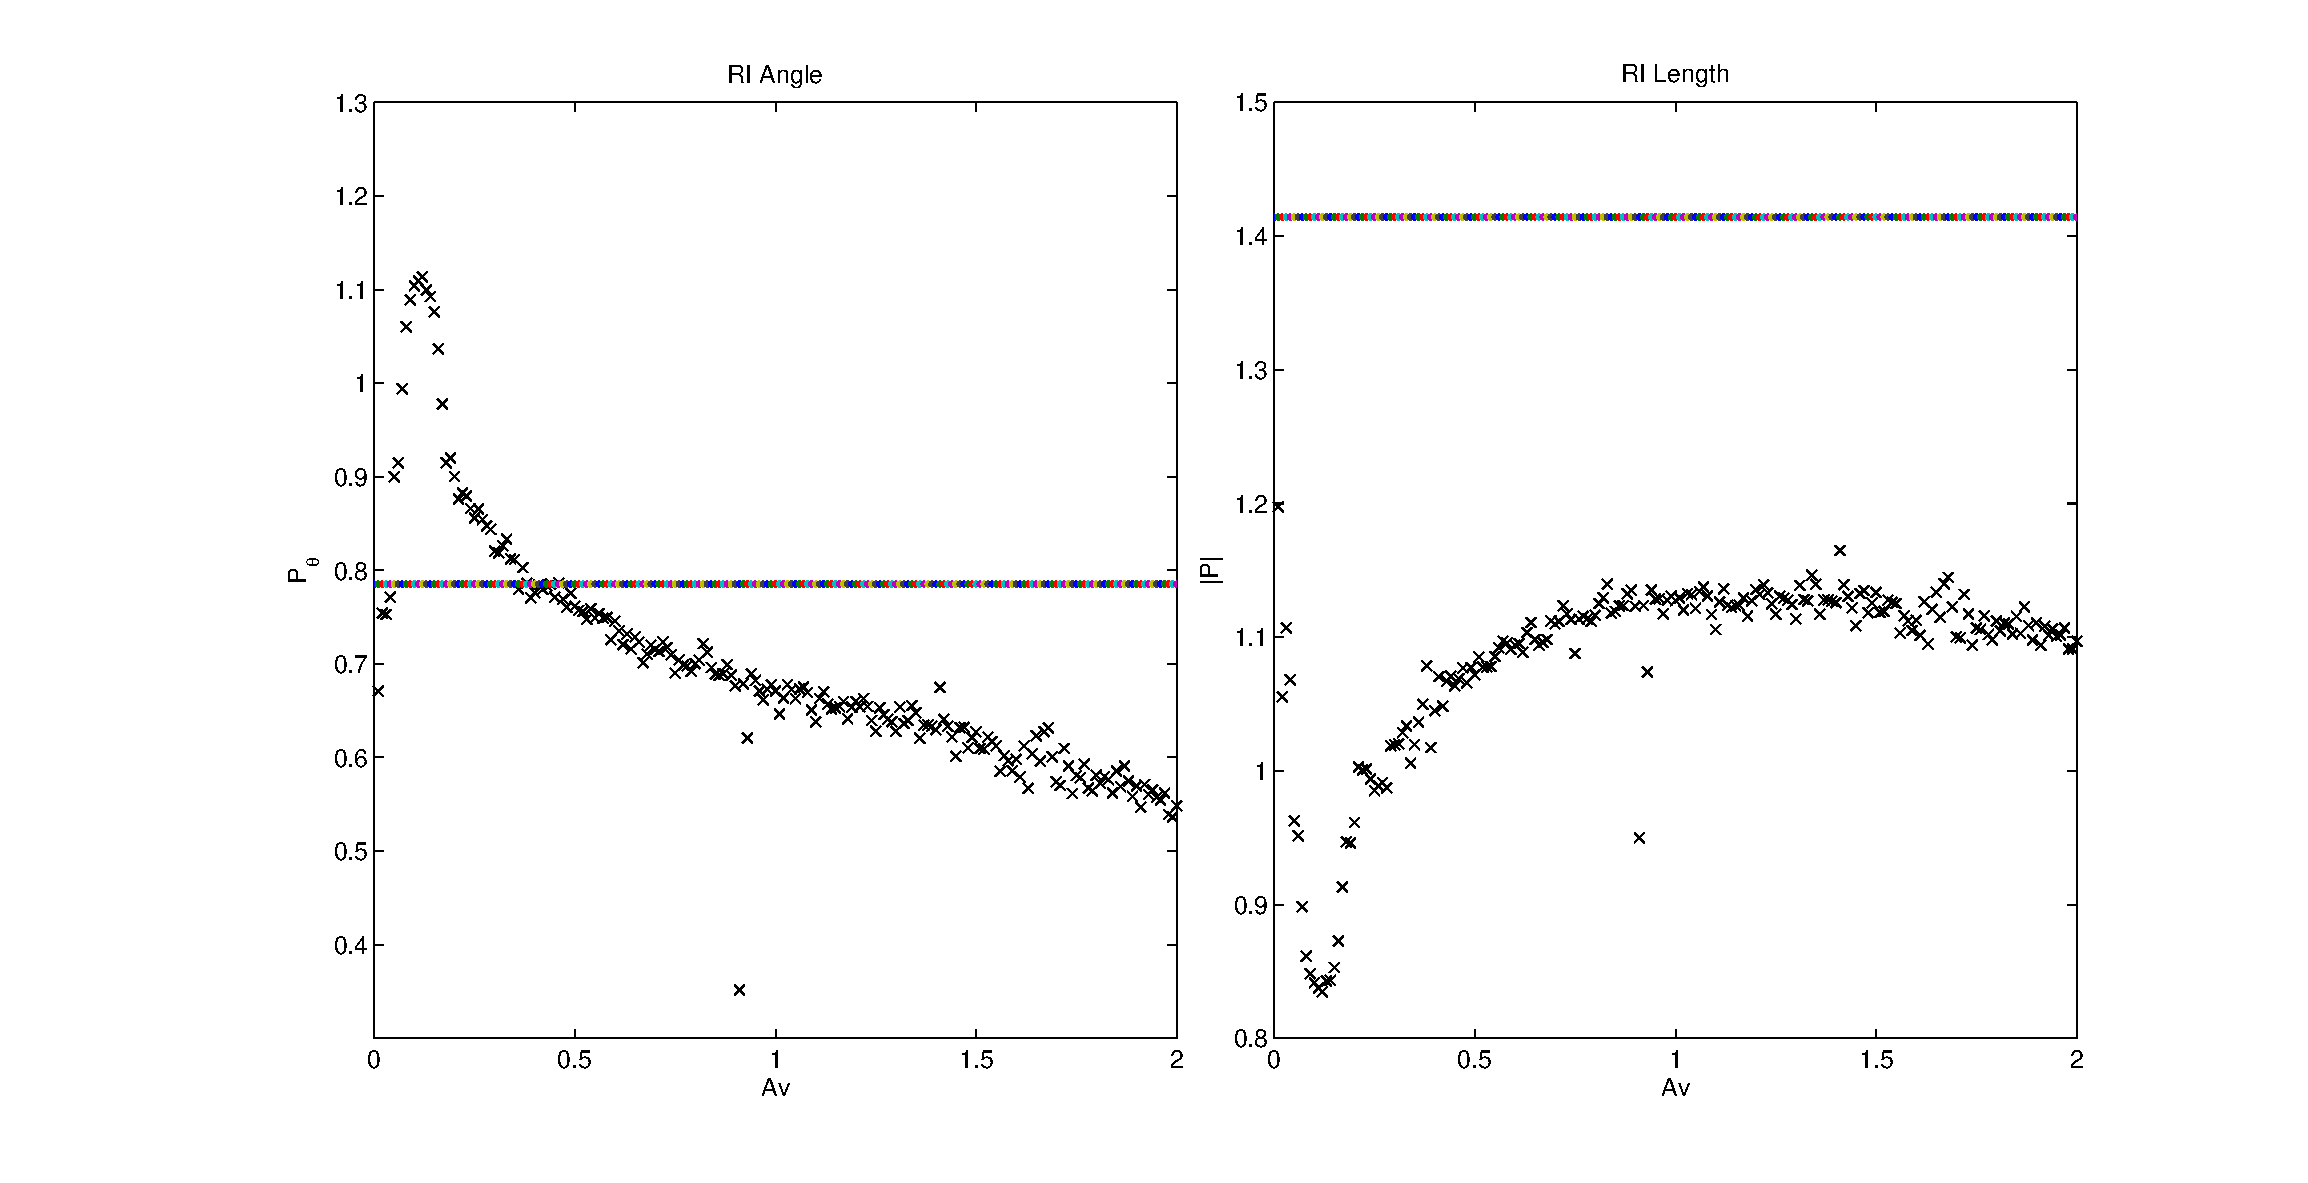
\includegraphics[scale=0.5]{RLcirc_varyR_amp.eps} \\
(b) $P_\theta$ and $|P|$ \\[6pt]
\end{tabular}
\caption{Changing $A_r$.}
\label{fig:Ar}
\end{figure}

\subsection{Changing $O_r$}
Consider evaluating the CCM correlations $C_{VI}$ and $C_{IV}$ for each $O_r\in[0.01,2.0]$ in steps of $0.01$.  For reference, both R(t) and I(t) are plotted for different $f_v$ in Figure \ref{fig:Orref}.
\begin{figure}[H]
%\includegraphics{}
\caption{Reference plots for changing $O_r$.}
\label{fig:Orref}
\end{figure}

The CCM correlations are each plotted in Figure \ref{fig:Or} along with the corresponding PAI elements $P_\theta$ and $|P|$.
\begin{figure}[H]
\begin{tabular}{cc}
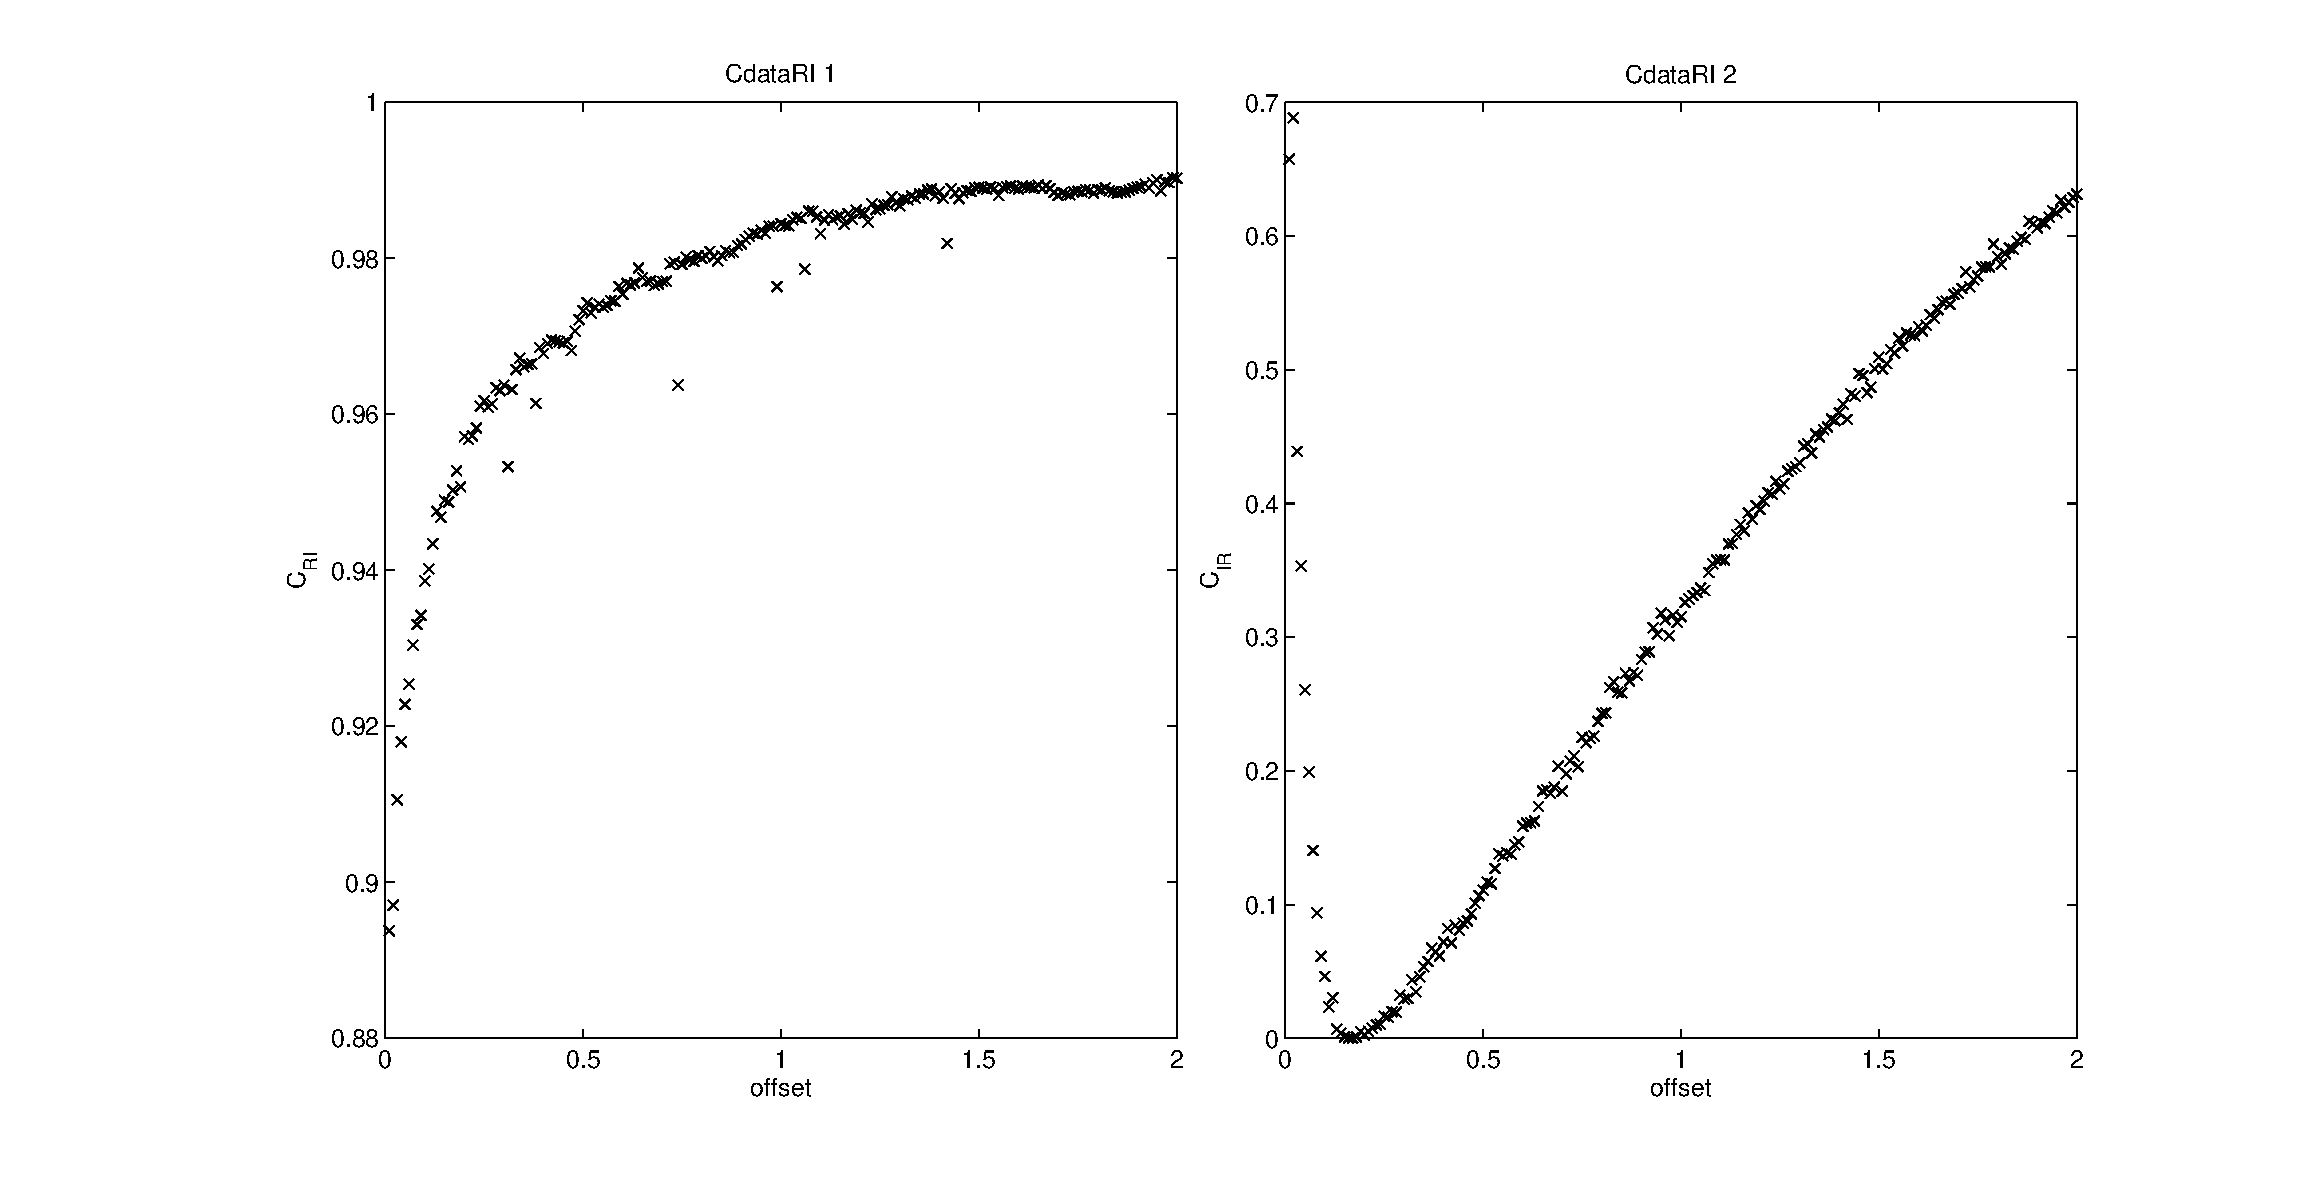
\includegraphics[scale=0.5]{RLcirc_varyR_offset2.eps} \\
(a) $C_{VI}$ and $C_{IV}$ \\[6pt]
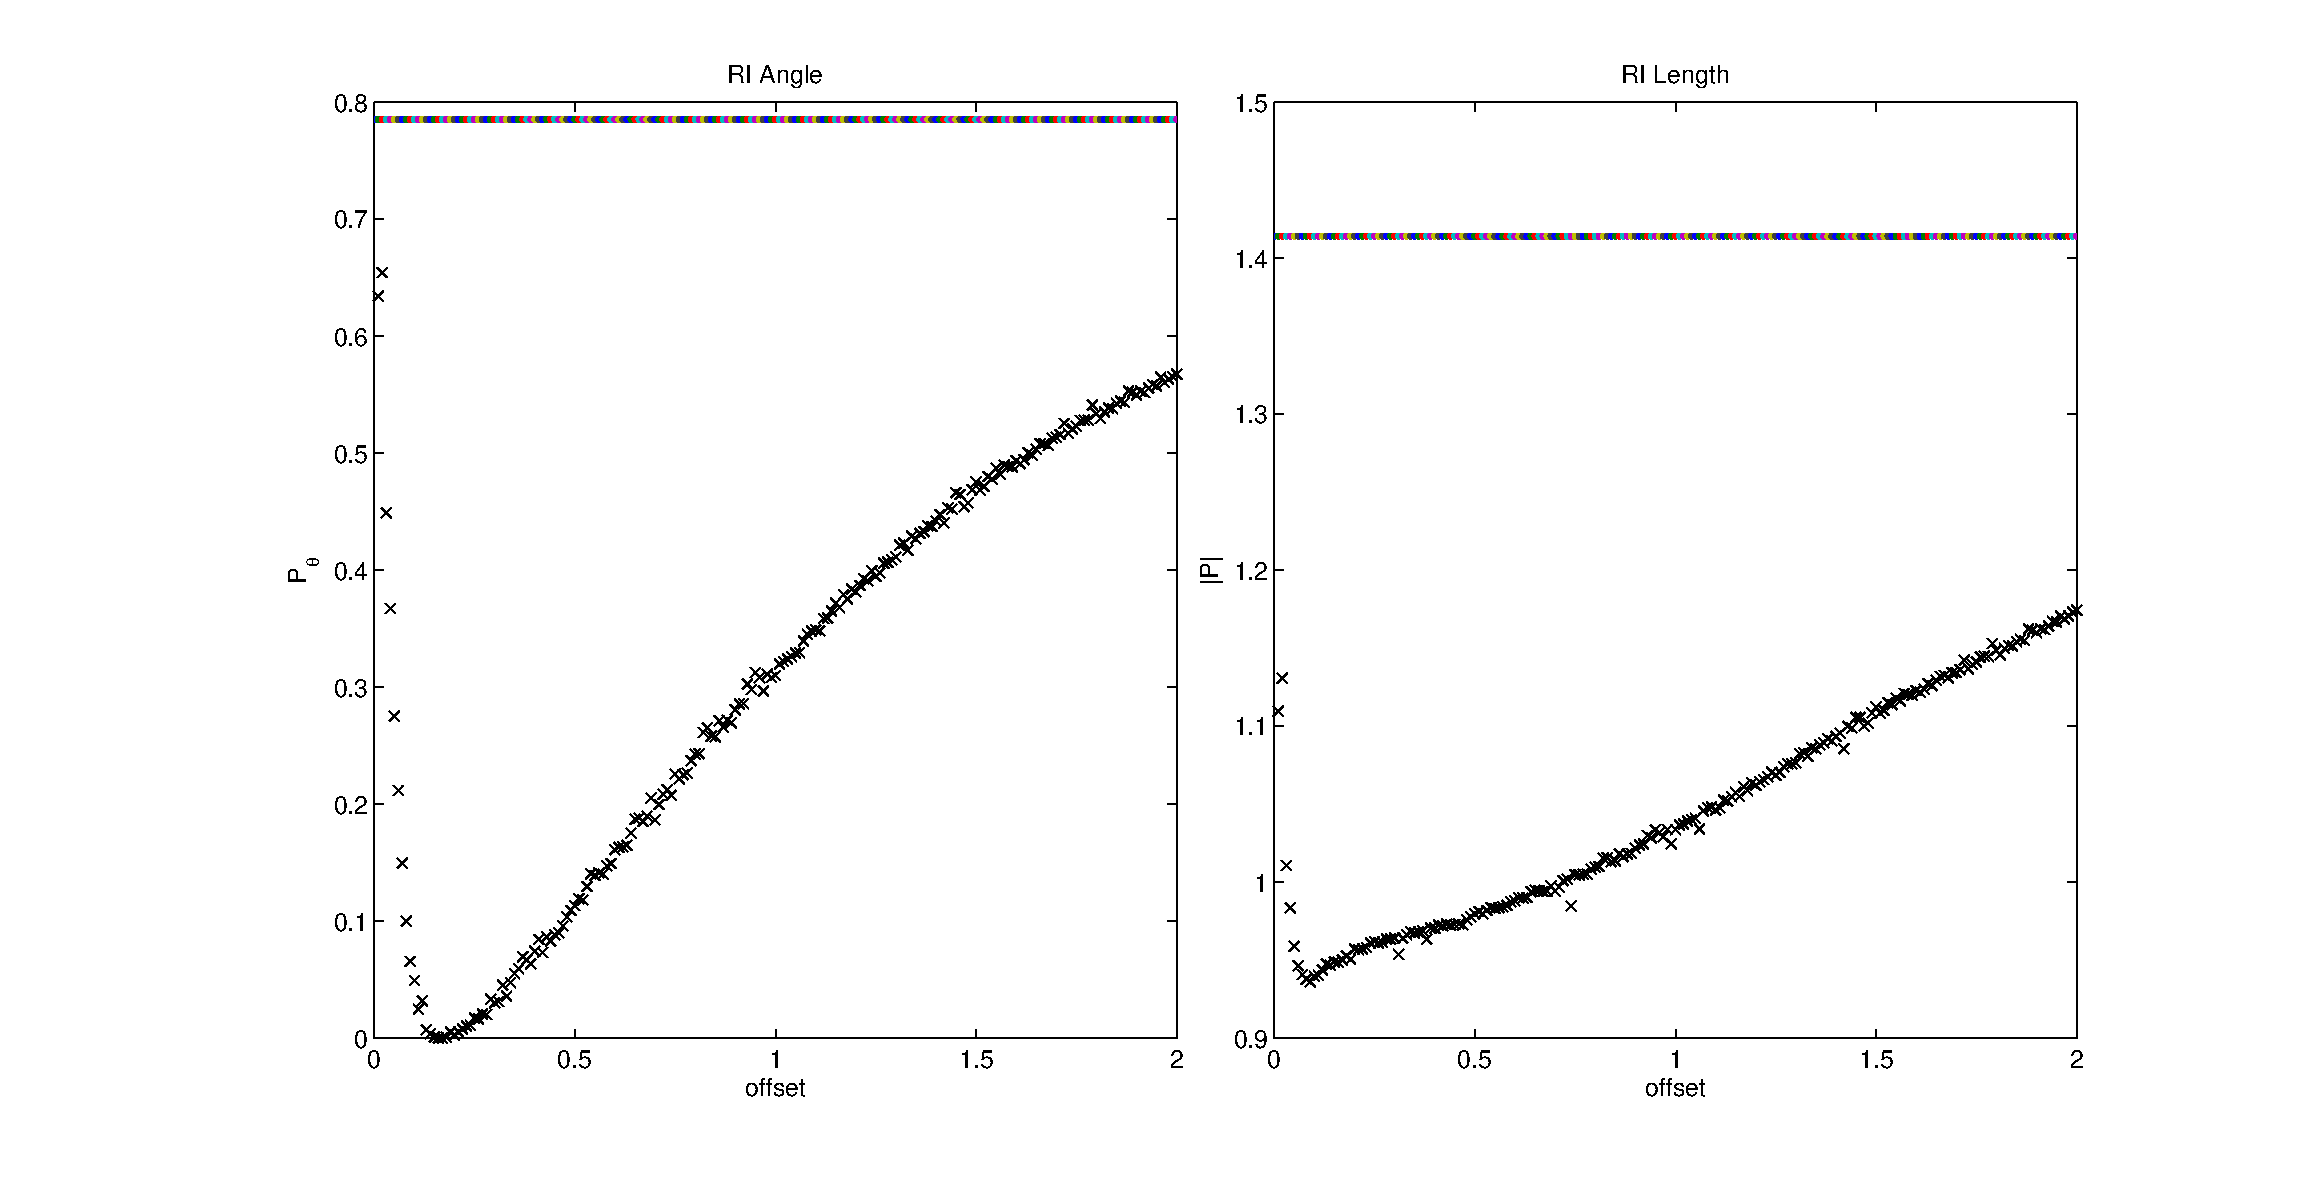
\includegraphics[scale=0.5]{RLcirc_varyR_offset.eps} \\
(b) $P_\theta$ and $|P|$ \\[6pt]
\end{tabular}
\caption{Changing $O_r$.}
\label{fig:Or}
\end{figure}

\subsection{Changing $\phi_r$}
Consider evaluating the CCM correlations $C_{VI}$ and $C_{IV}$ for each $\phi_r\in[0.01,2.0]$ in steps of $0.01$.  For reference, both R(t) and I(t) are plotted for different $\phi_r$ in Figure \ref{fig:Prref}.
\begin{figure}[H]
%\includegraphics{}
\caption{Reference plots for changing $\phi_r$.}
\label{fig:Prref}
\end{figure}

The CCM correlations are each plotted in Figure \ref{fig:Pr} along with the corresponding PAI elements $P_\theta$ and $|P|$.
\begin{figure}[H]
\begin{tabular}{cc}
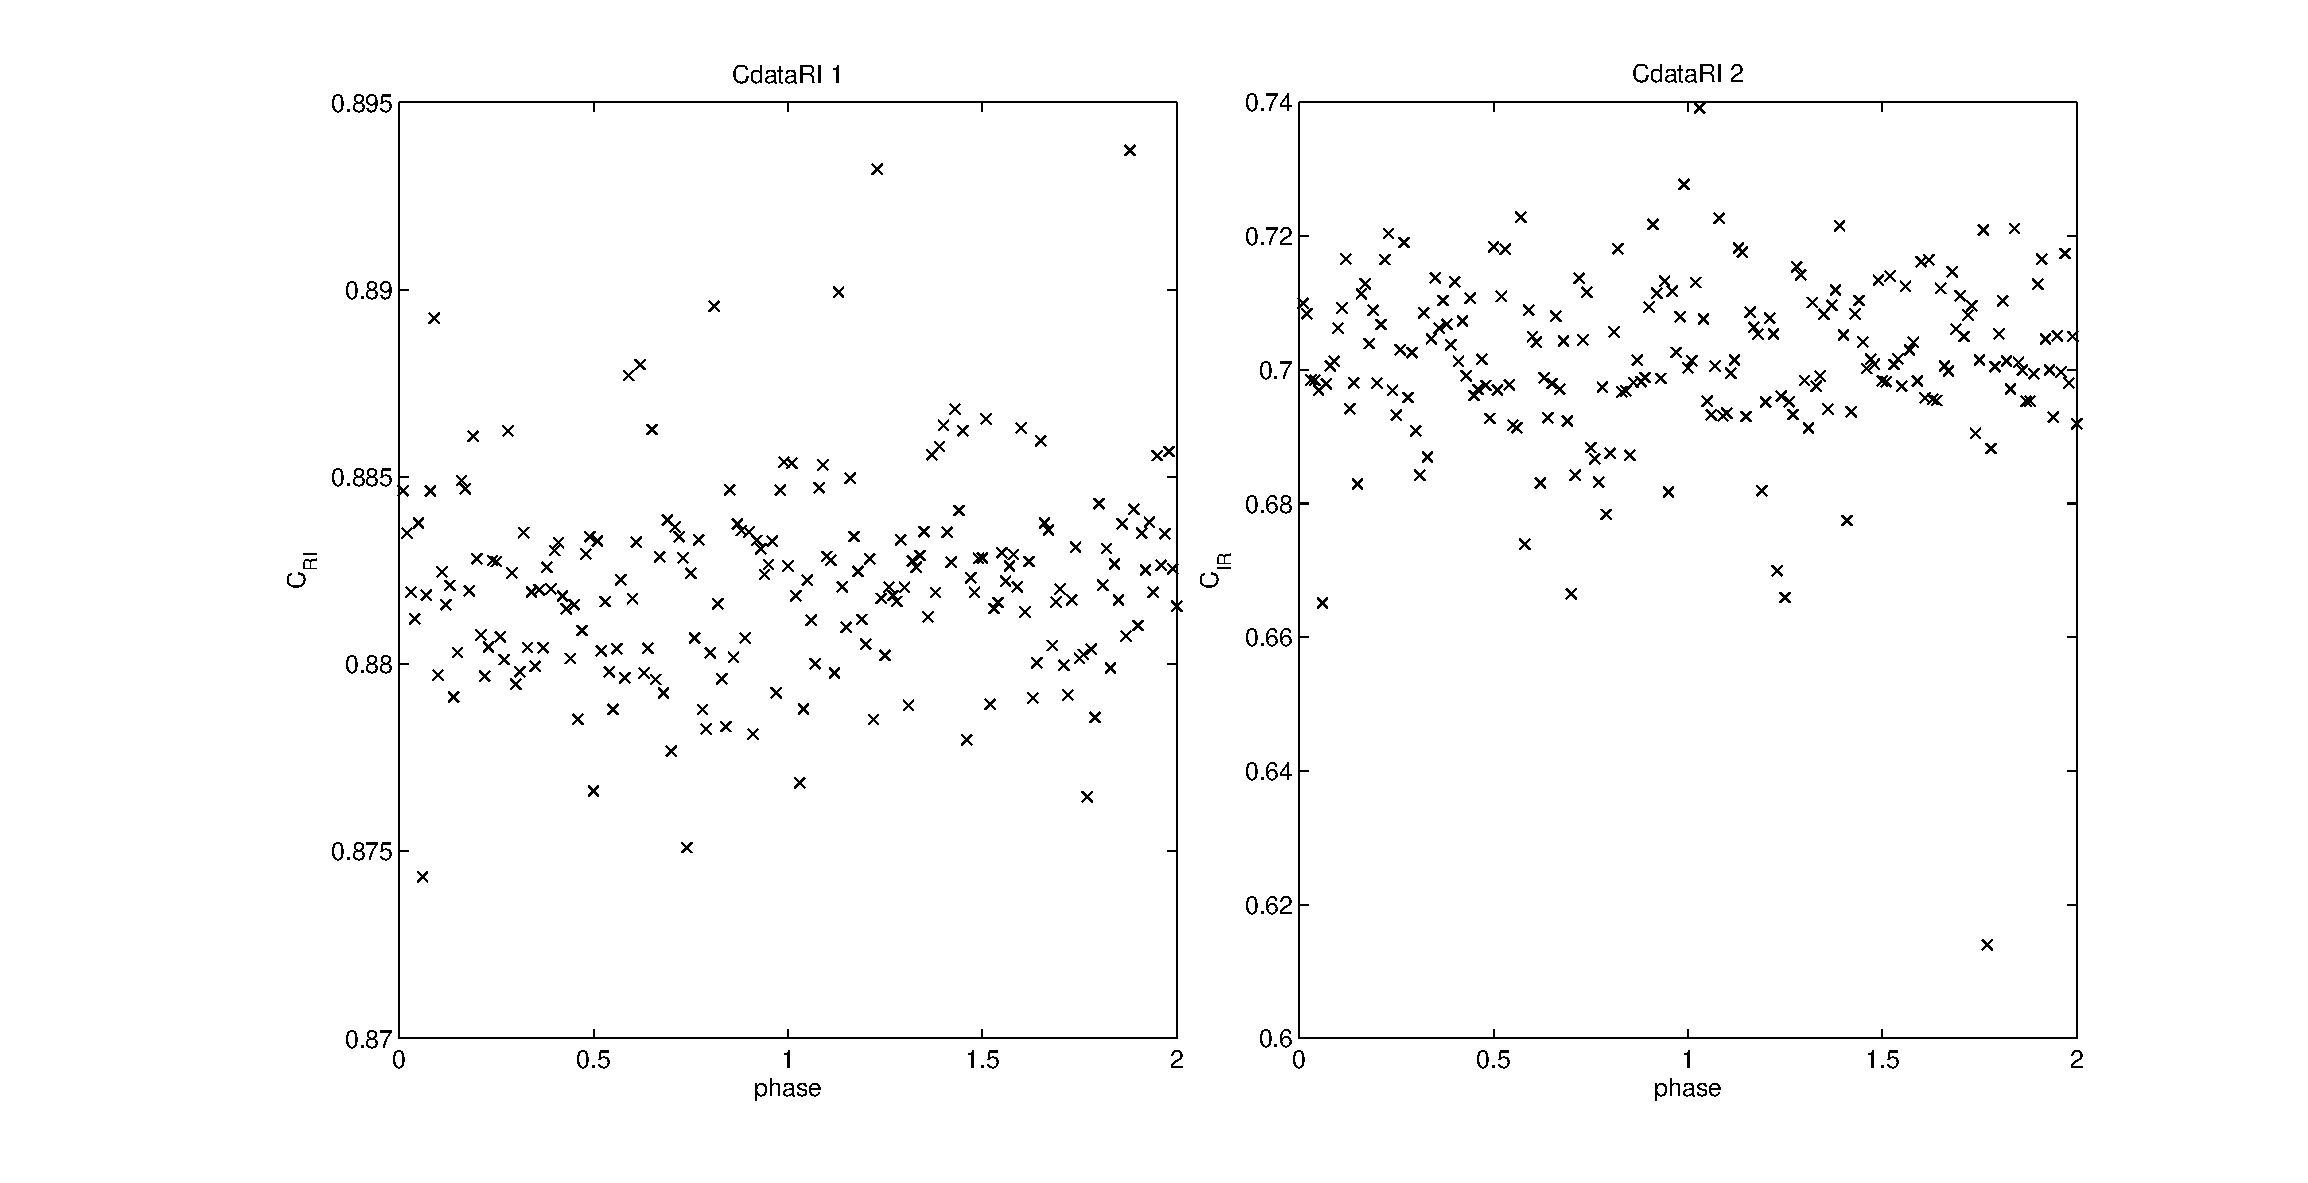
\includegraphics[scale=0.5]{RLcirc_varyR_phase2.eps} \\
(a) $C_{VI}$ and $C_{IV}$ \\[6pt]
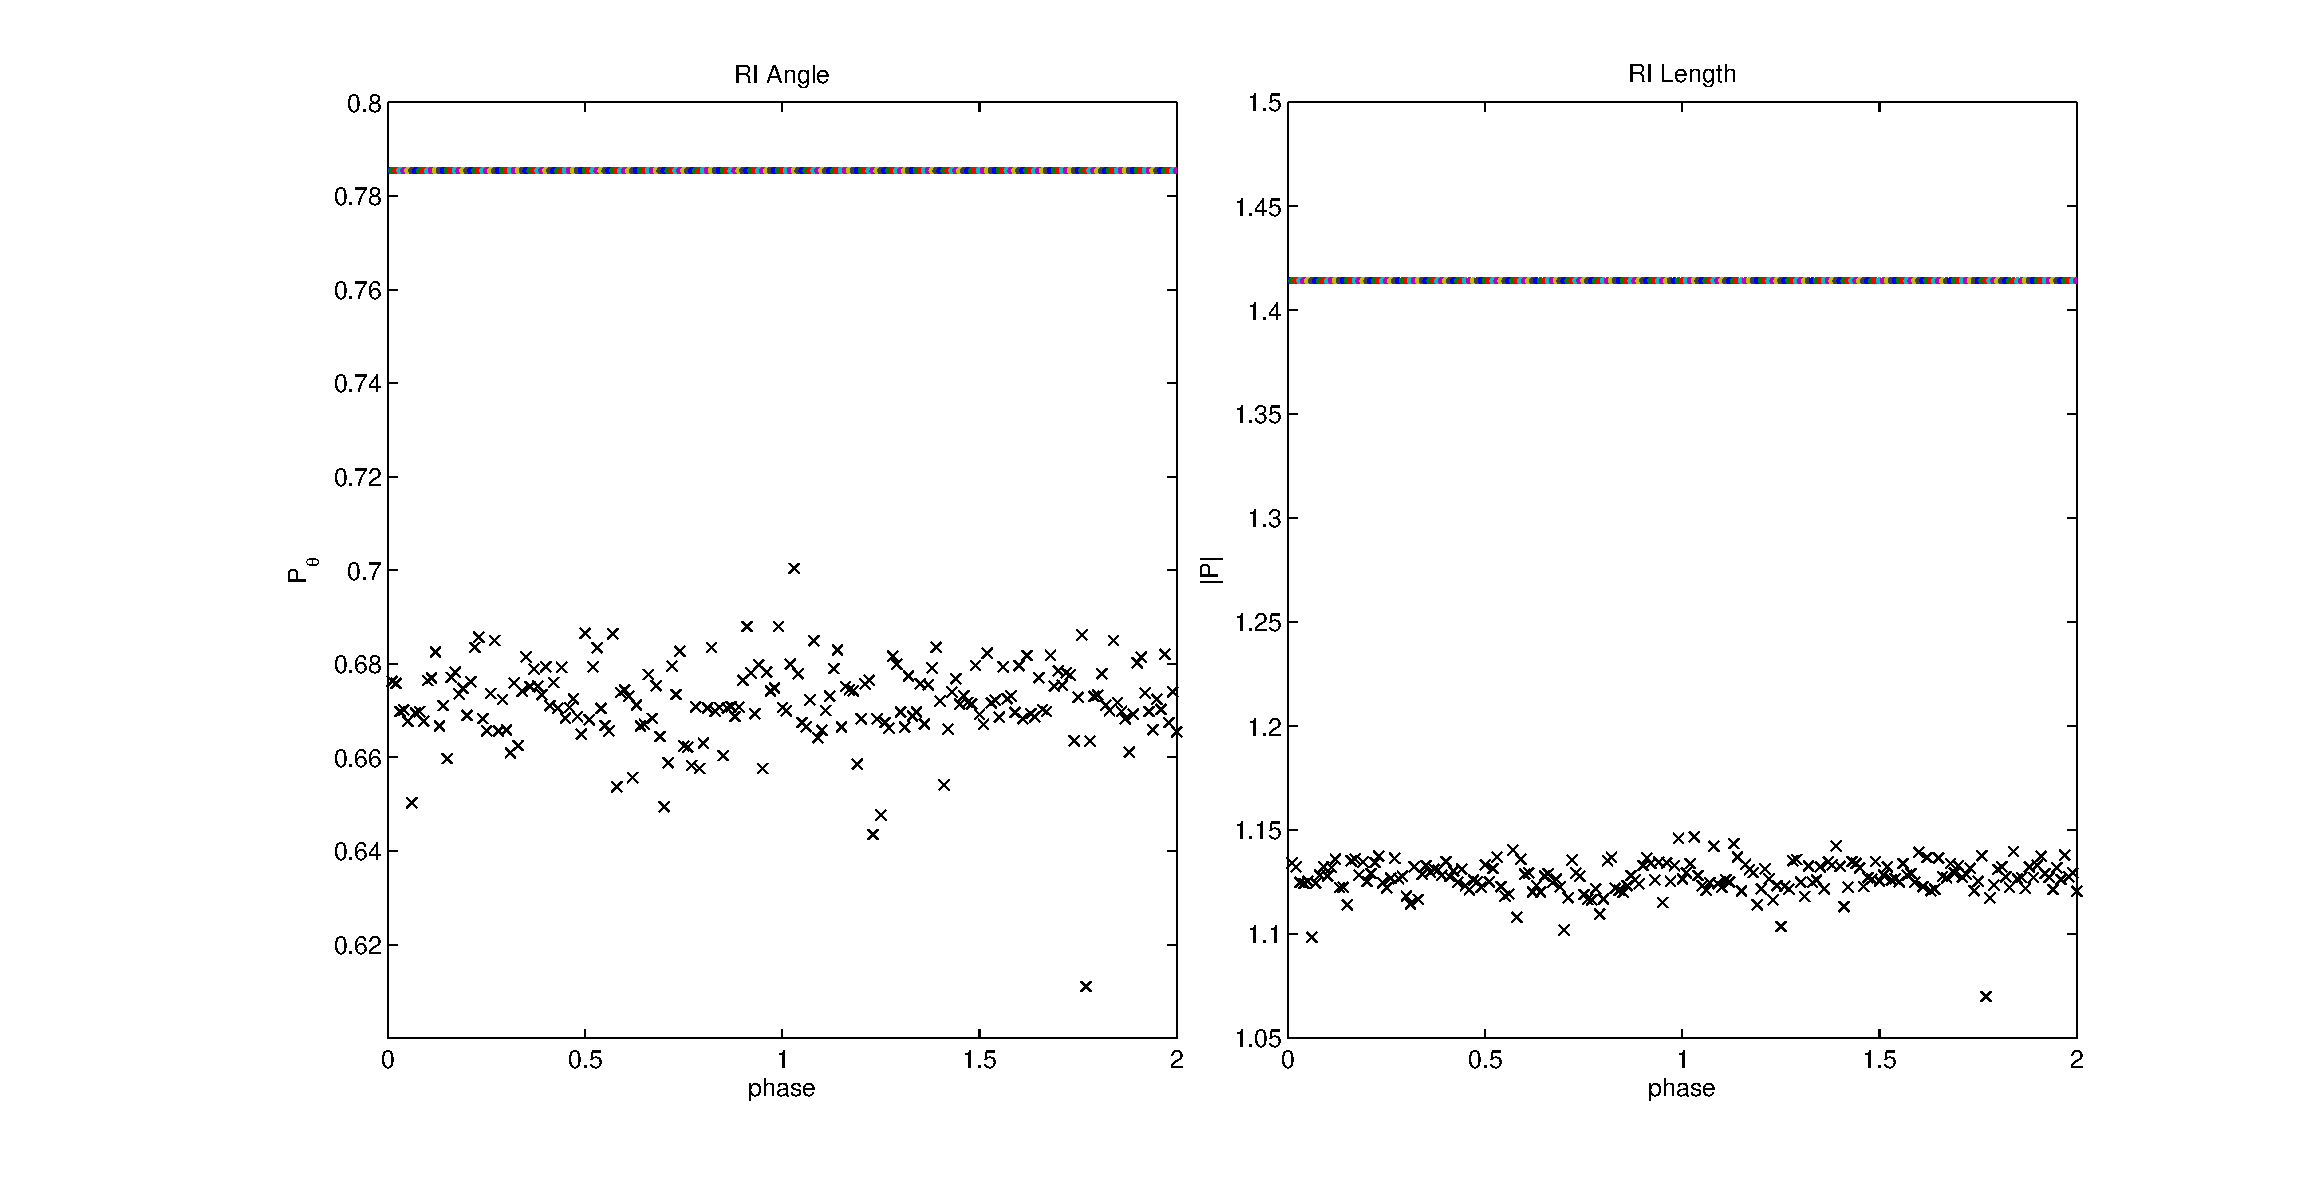
\includegraphics[scale=0.5]{RLcirc_varyR_phase.eps} \\
(b) $P_\theta$ and $|P|$ \\[6pt]
\end{tabular}
\caption{Changing $\phi_r$.}
\label{fig:Pv}
\end{figure}

\subsection{Changing $f_r$}
Consider evaluating the CCM correlations $C_{VI}$ and $C_{IV}$ for each $f_r\in[0.01,2.0]$ in steps of $0.01$.  For reference, both R(t) and I(t) are plotted for different $f_r$ in Figure \ref{fig:frref}.
\begin{figure}[H]
%\includegraphics{}
\caption{Reference plots for changing $f_r$.}
\label{fig:frref}
\end{figure}

The CCM correlations are each plotted in Figure \ref{fig:fr} along with the corresponding PAI elements $P_\theta$ and $|P|$.
\begin{figure}[H]
\begin{tabular}{cc}
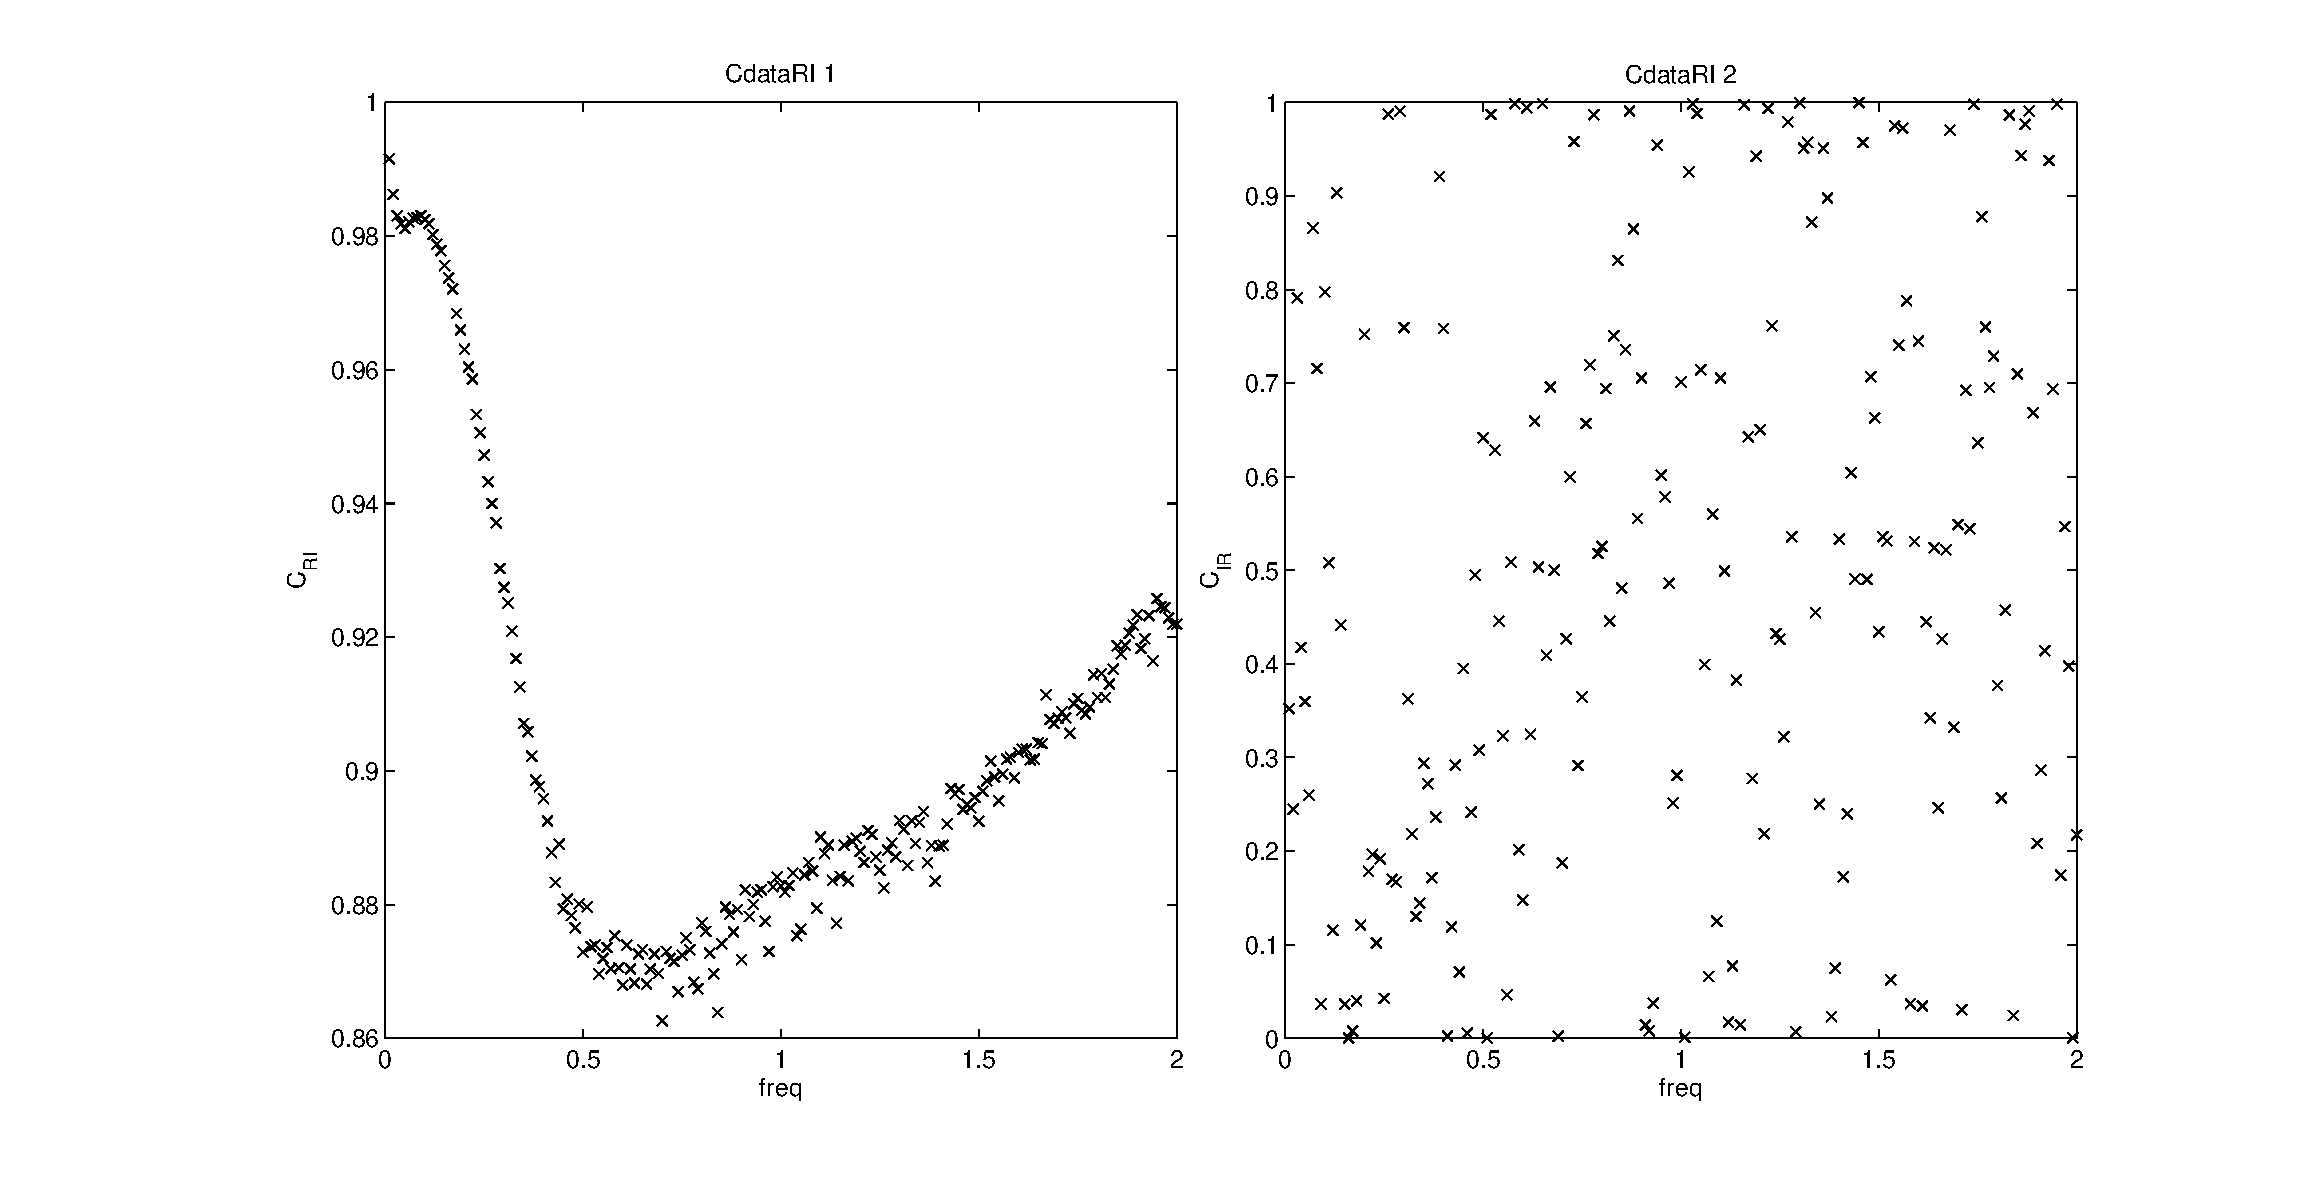
\includegraphics[scale=0.5]{RLcirc_varyR_freq2.eps} \\
(a) $C_{VI}$ and $C_{IV}$ \\[6pt]
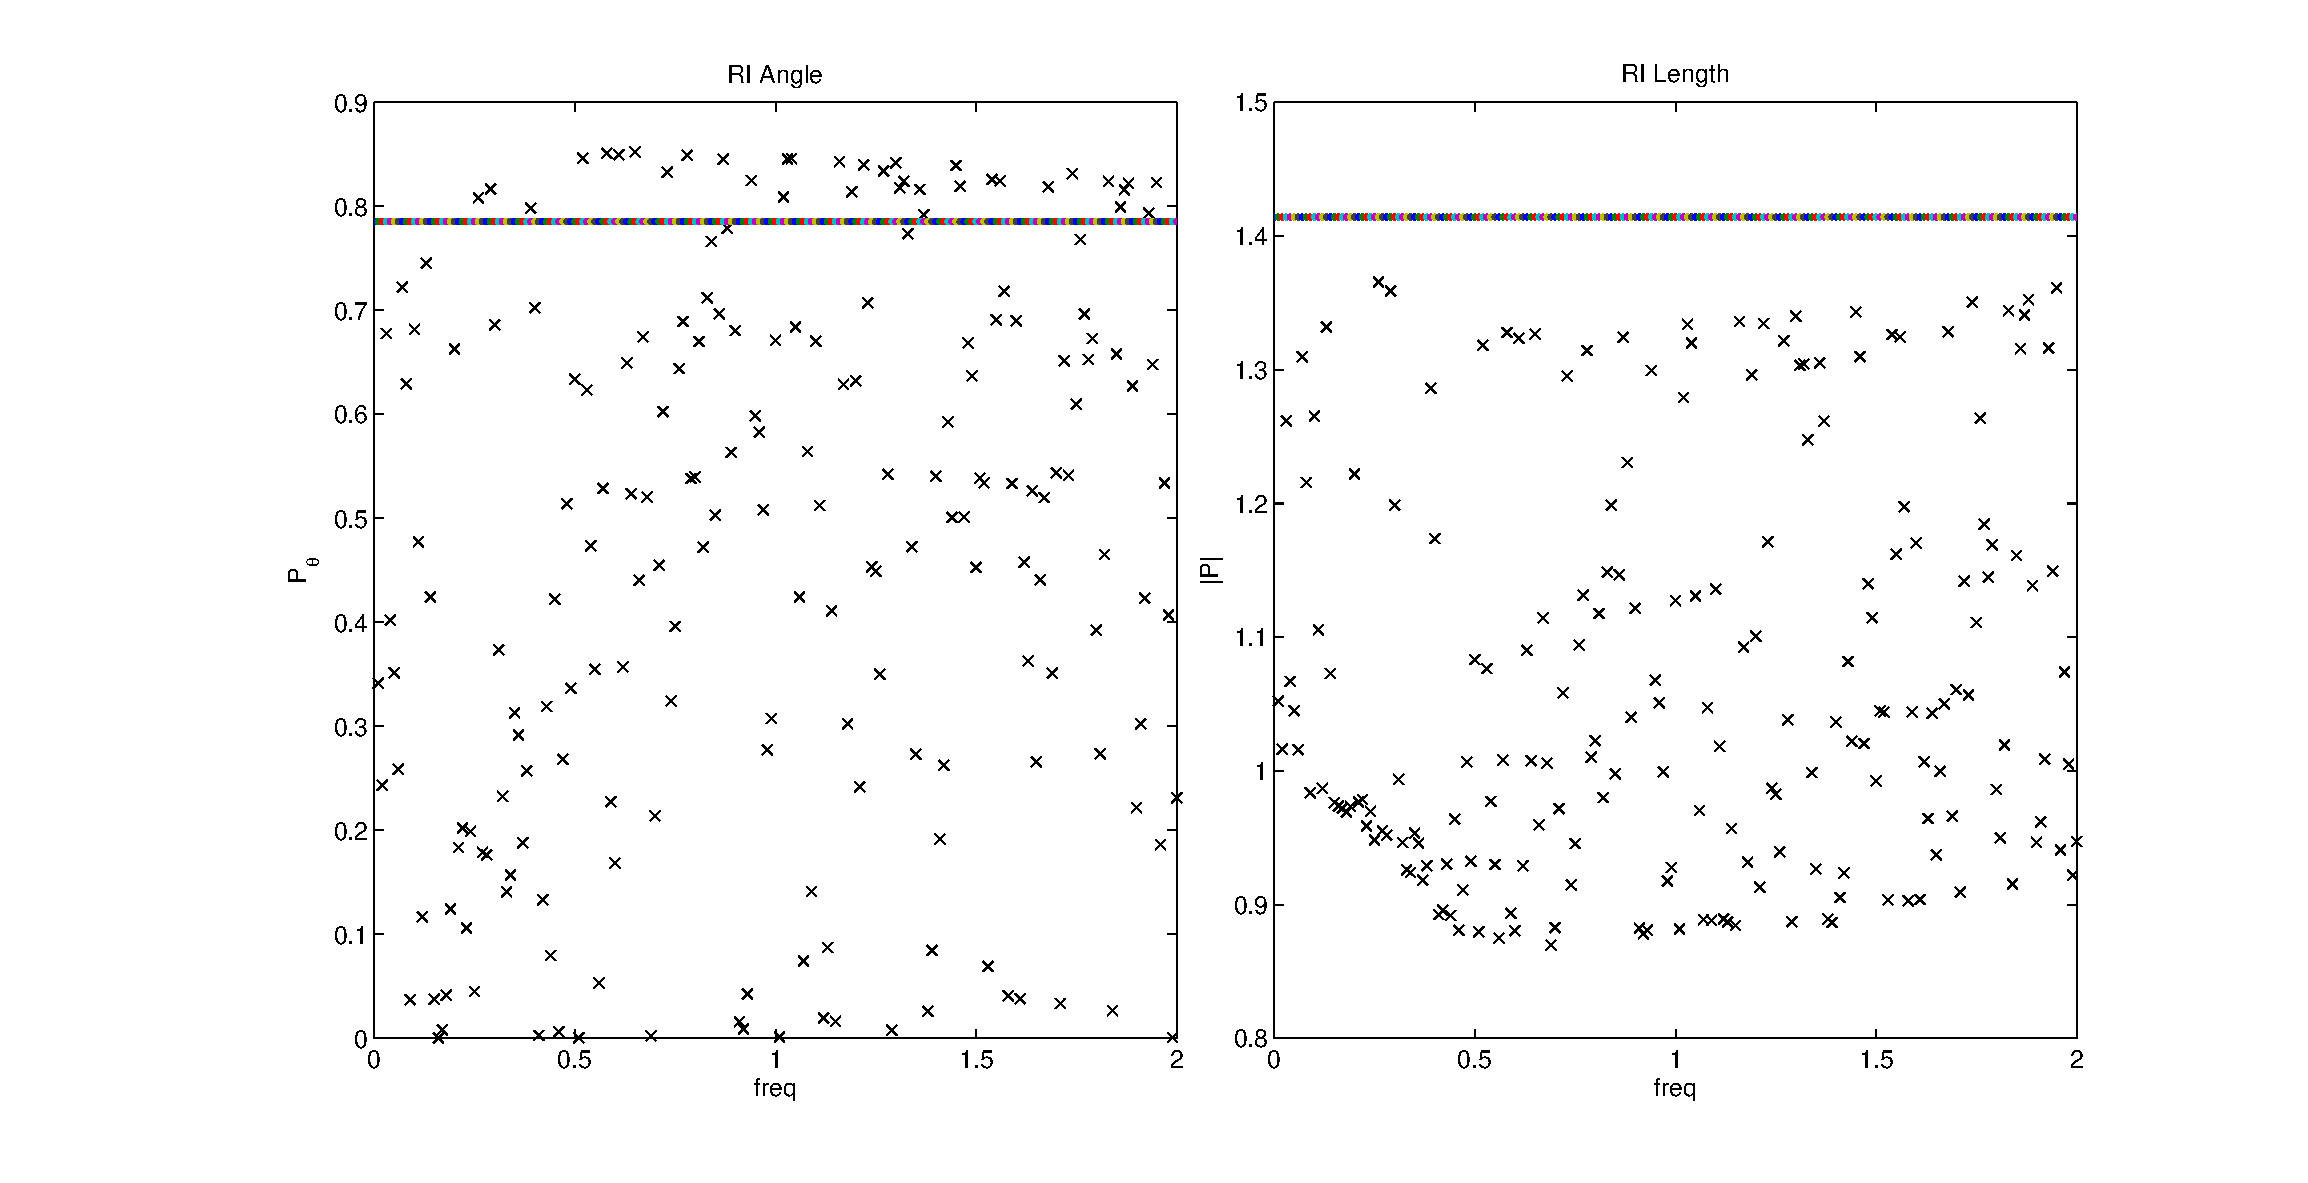
\includegraphics[scale=0.5]{RLcirc_varyR_freq.eps} \\
(b) $P_\theta$ and $|P|$ \\[6pt]

\end{tabular}
\caption{Changing $f_r$.}
\label{fig:fr}
\end{figure}

Figure \ref{fig:fr1} shows the effect of increasing the library length from $2\times10^3$ (i.e.\ {\tt tspan = [0:0.5:1000];}) to $10^4$ (i.e.\ {\tt tspan = [0:0.5:5000];}), and Figure \ref{fig:fr2} extends the above plots to $f_r\in[0.01,10.0]$ in steps of $0.05$.
\begin{figure}[H]
\begin{tabular}{cc}
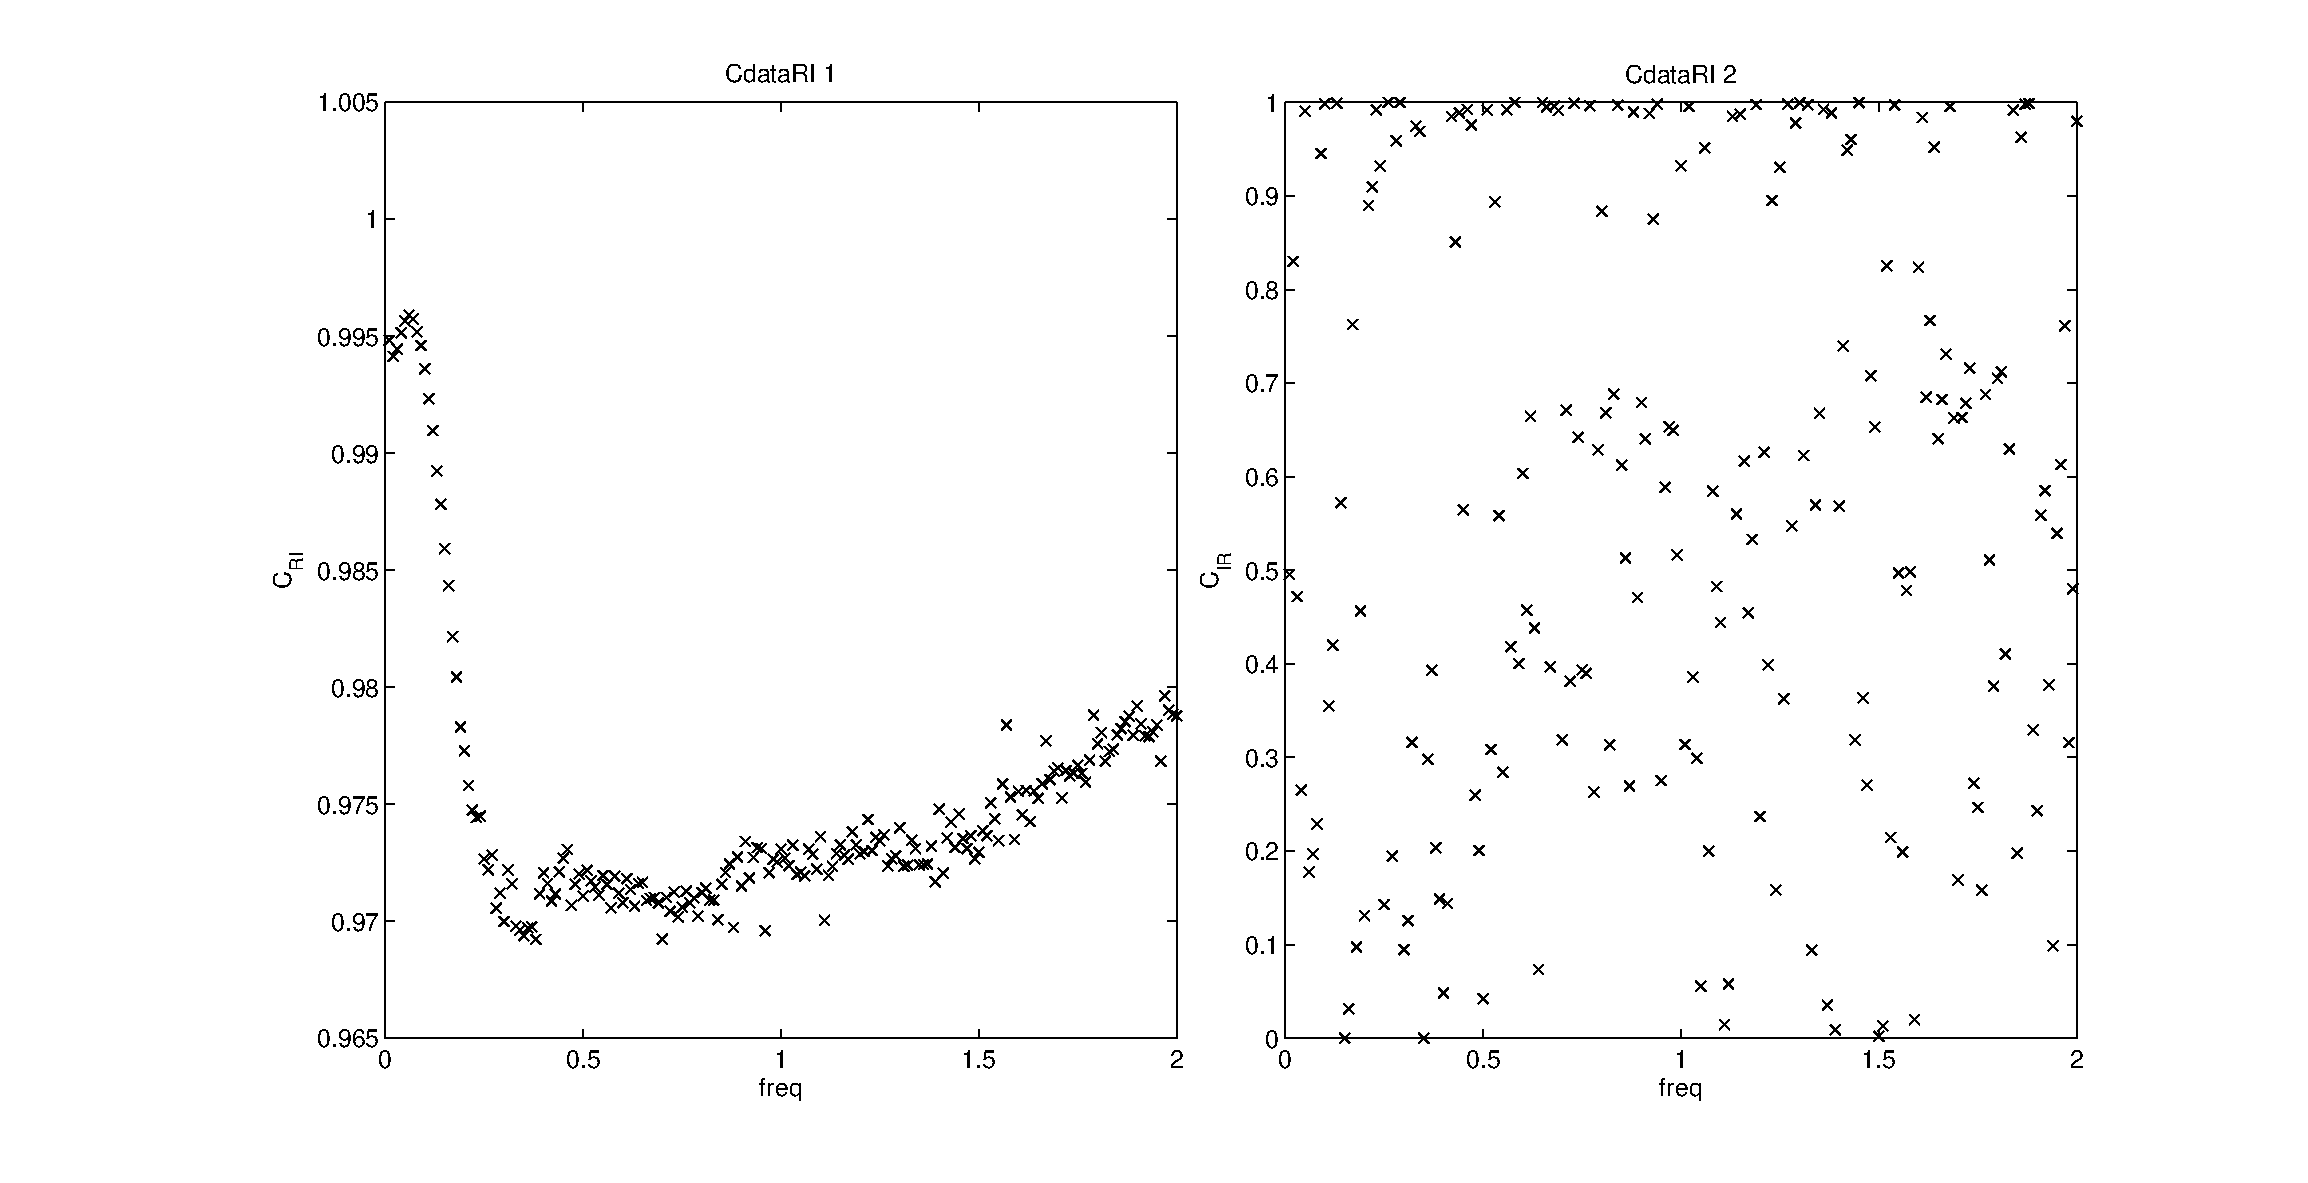
\includegraphics[scale=0.5]{RLcirc_varyR_freqLup2.eps} \\
(a) $C_{VI}$ and $C_{IV}$ \\[6pt]
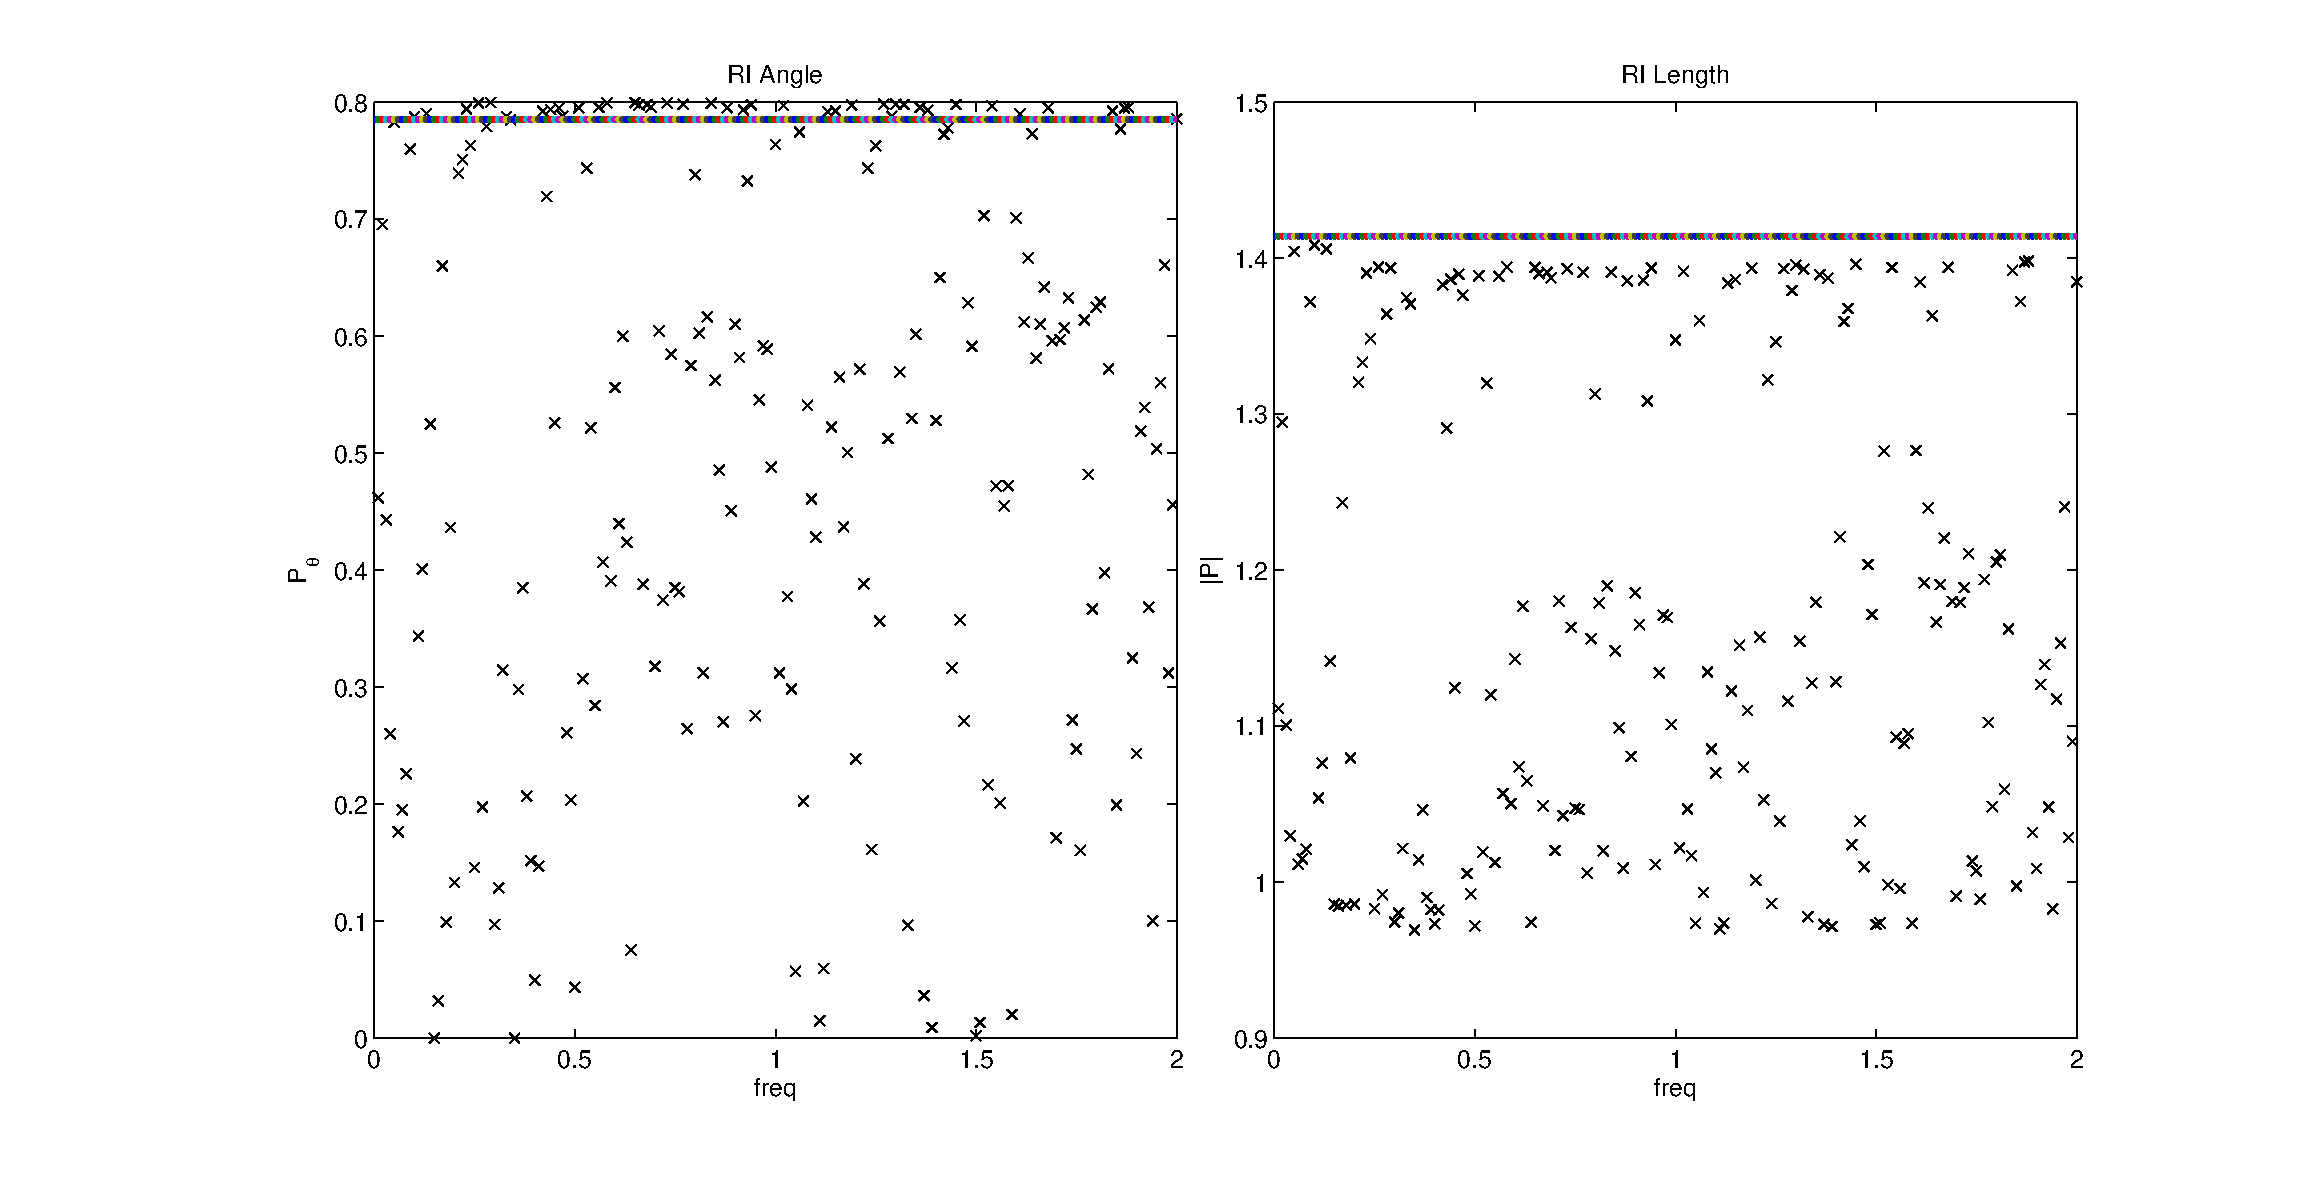
\includegraphics[scale=0.5]{RLcirc_varyR_freqLup.eps} \\
(b) $P_\theta$ and $|P|$ \\[6pt]
\end{tabular}
\caption{Changing $f_r$ (longer library length).}
\label{fig:fr1}
\end{figure}
\begin{figure}[H]
\begin{tabular}{cc}
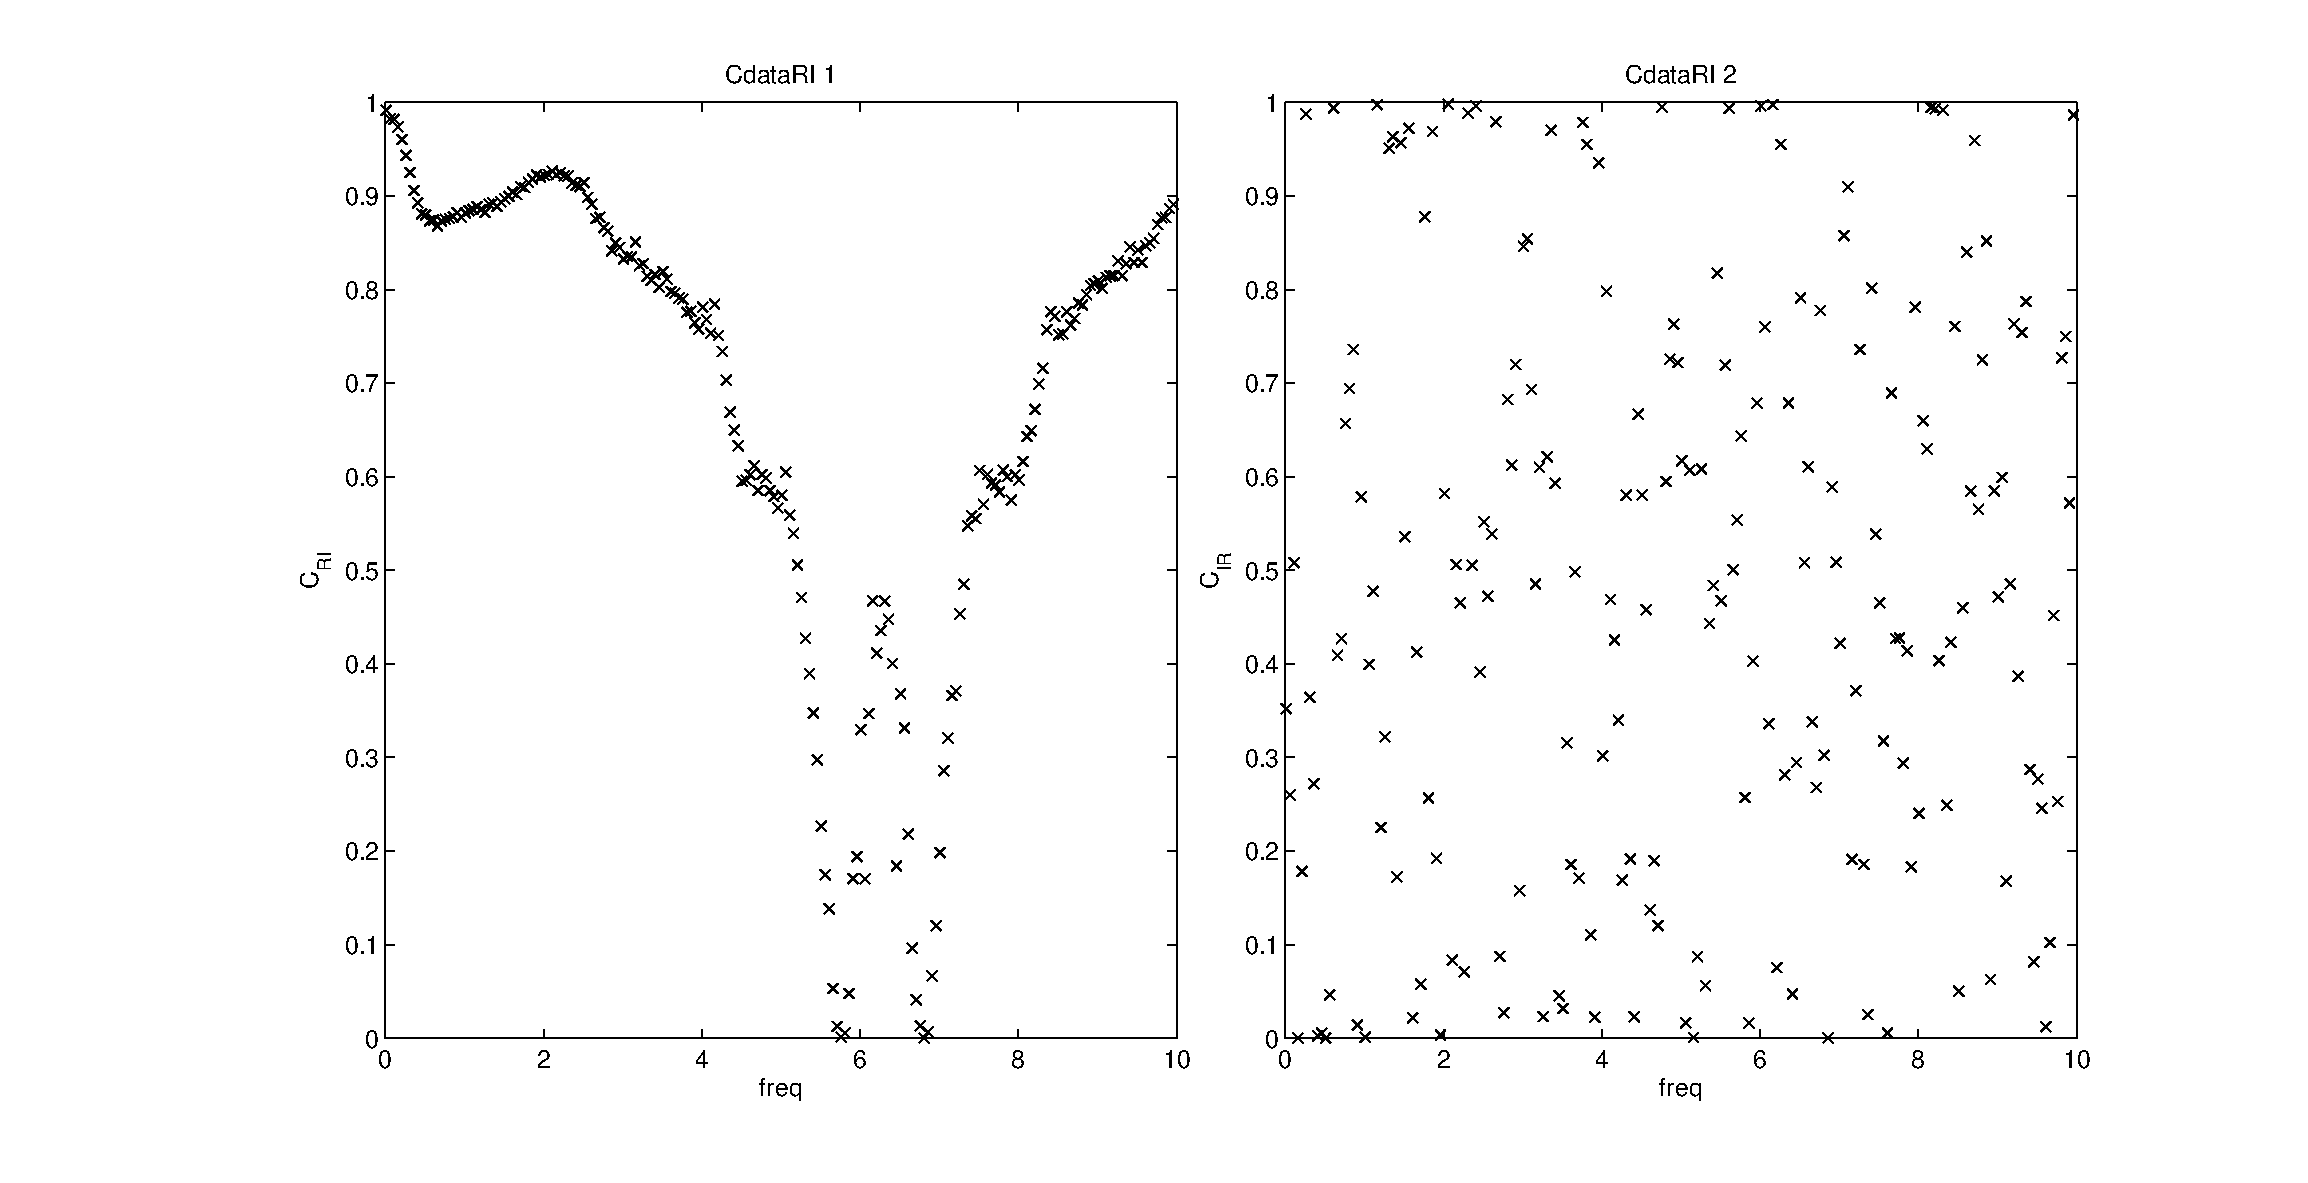
\includegraphics[scale=0.5]{RLcirc_varyR_freqlong2.eps} \\
(a) $C_{VI}$ and $C_{IV}$ \\[6pt]
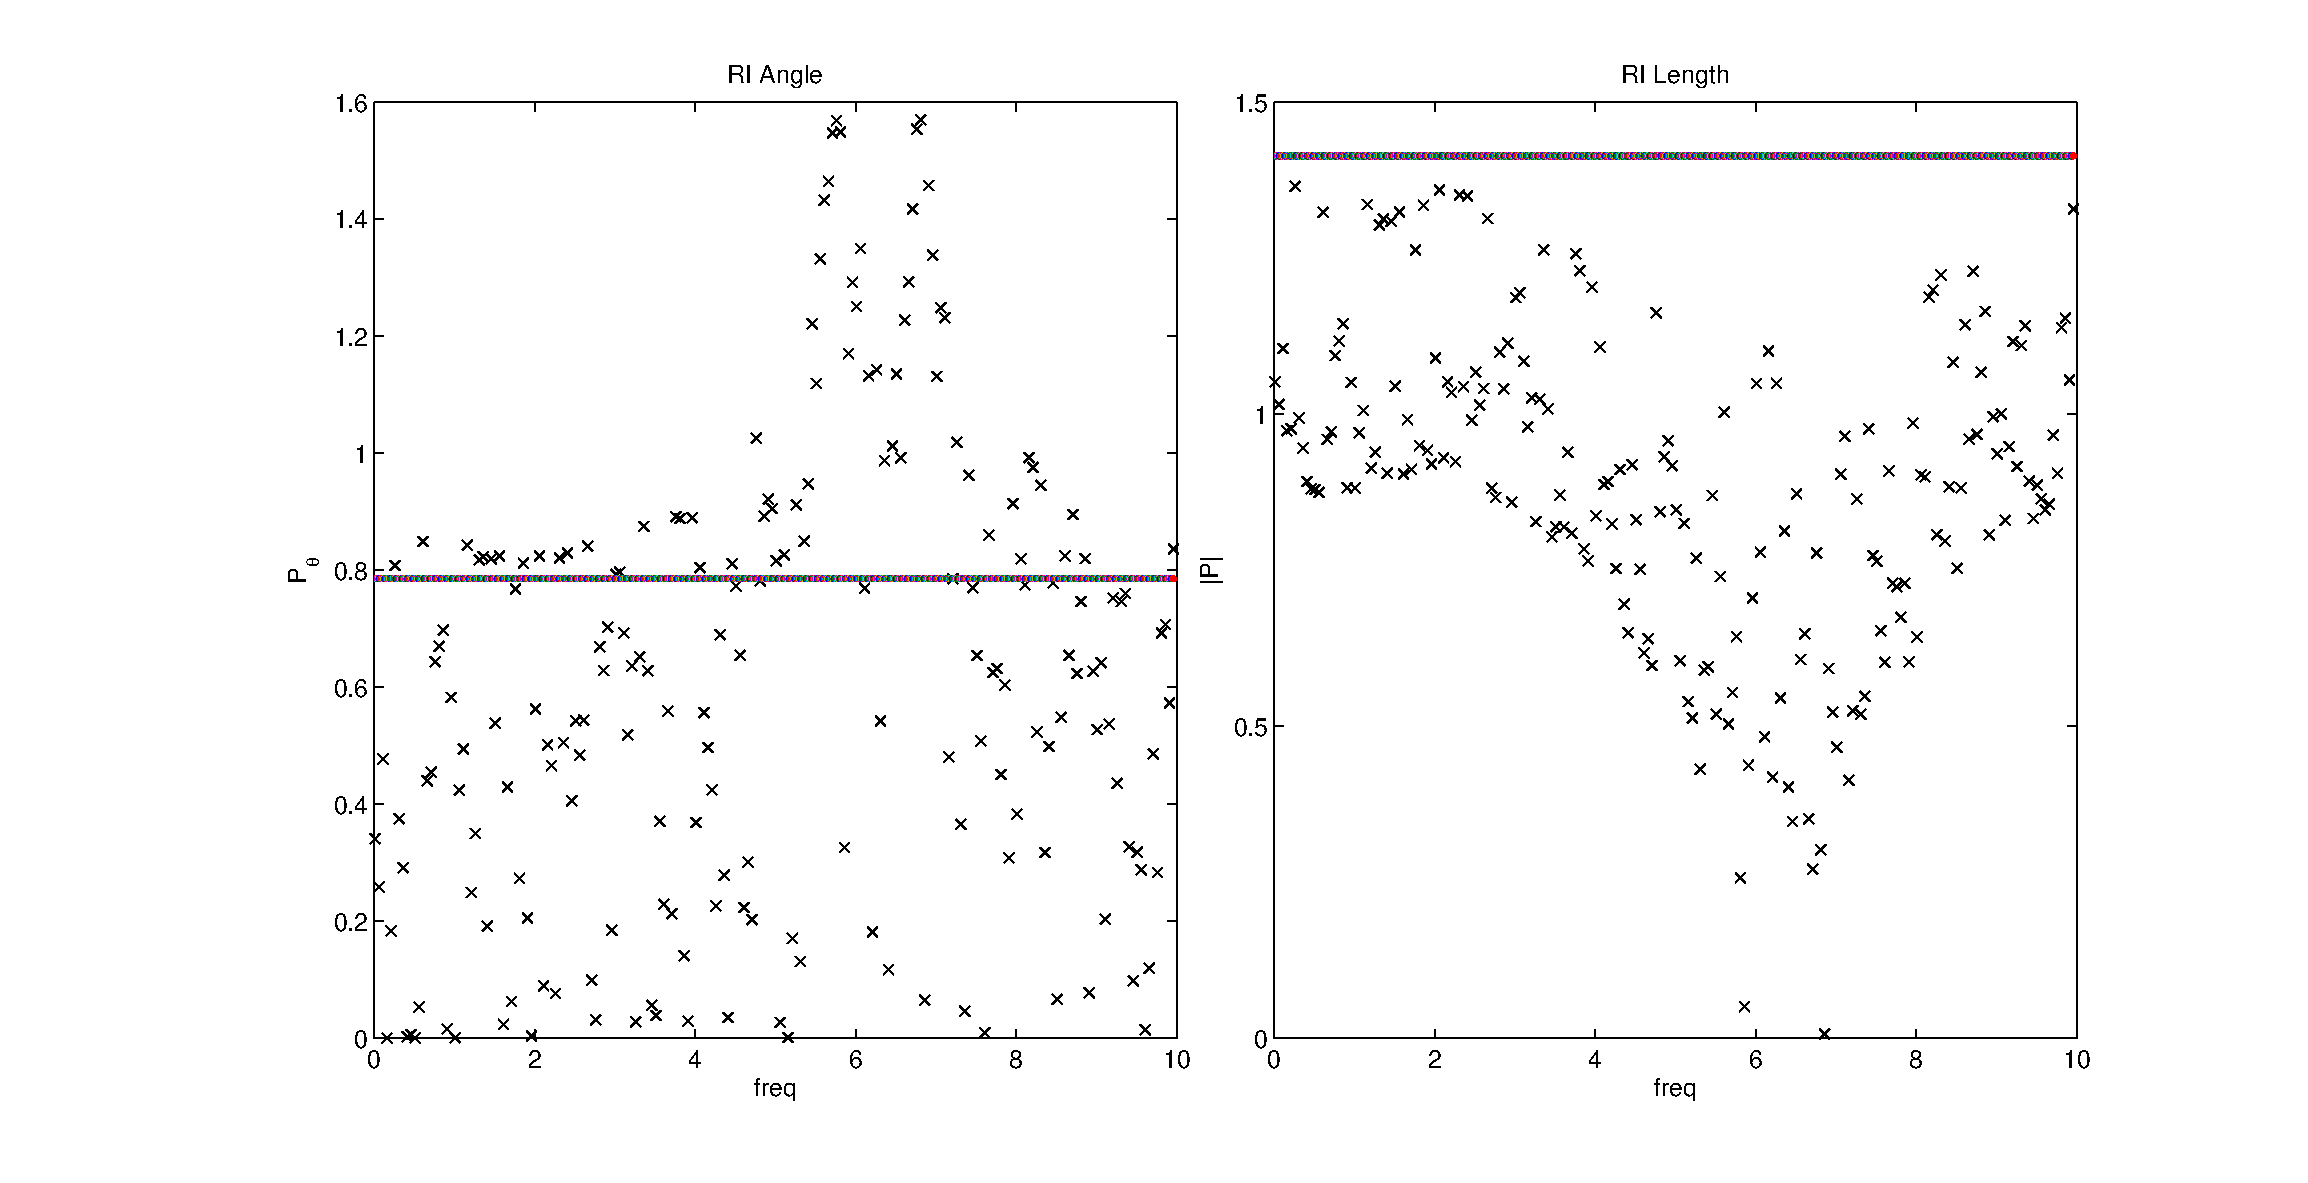
\includegraphics[scale=0.5]{RLcirc_varyR_freqlong.eps} \\
(b) $P_\theta$ and $|P|$ \\[6pt]
\end{tabular}
\caption{Changing $f_r$ (larger domain for $f_r$).}
\label{fig:fr2}
\end{figure}
\end{comment}

---
\section{PAI}
Consider the system (Sugihara Figure 3 C and D)
\begin{eqnarray}
X_{t+1} &=& X_t\left(r_x-r_xX_t-\beta_{xy}Y_t\right)\\
Y_{t+1} &=& Y_t\left(r_y-r_yY_t-\beta_{yx}X_t\right),
\end{eqnarray}
with $r_y=r_y=3.7$, $X_0 = 0.2$, $Y_0=0.4$, $\beta_{xy}=0$, and $\beta_{yx}=0.32$.  Plots of the correlation between $X$ and $X|Y$, as well as, $Y$ and $Y|X$ are shown below.
\begin{center}
\begin{figure}[H]
\begin{tabular}{cc}
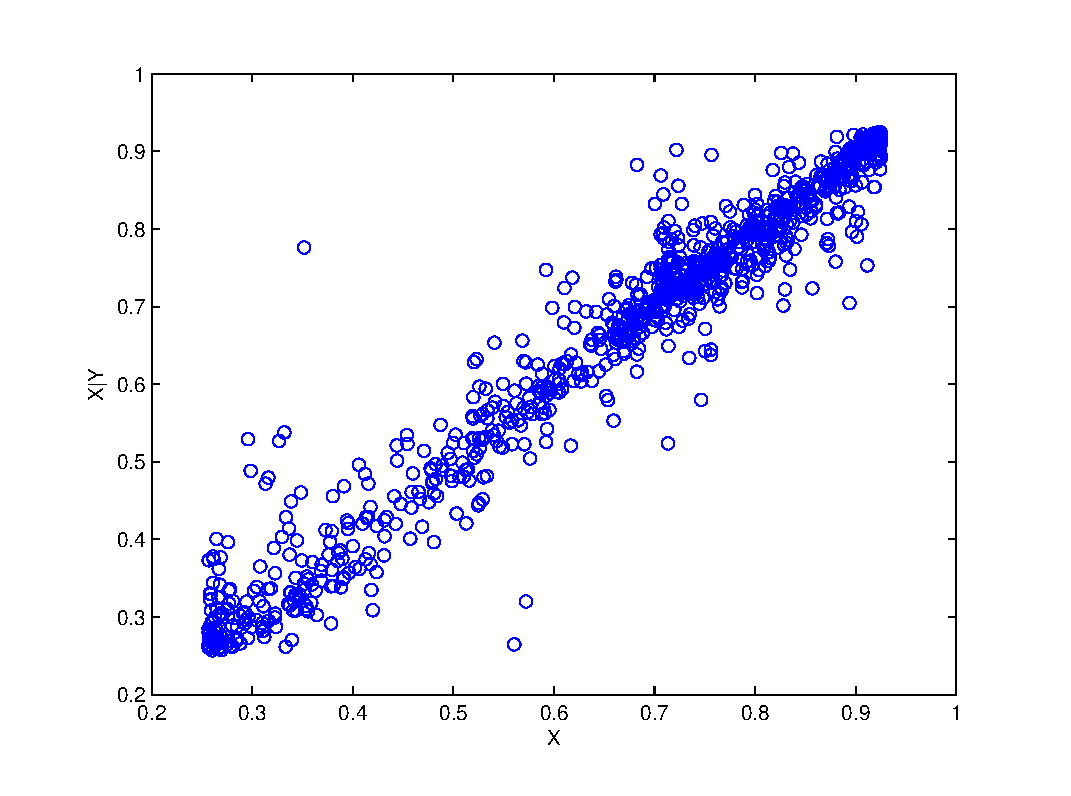
\includegraphics[scale=0.5]{SugFig3_XgY.eps} \\
(a) $C_{XY}$ \\[6pt]
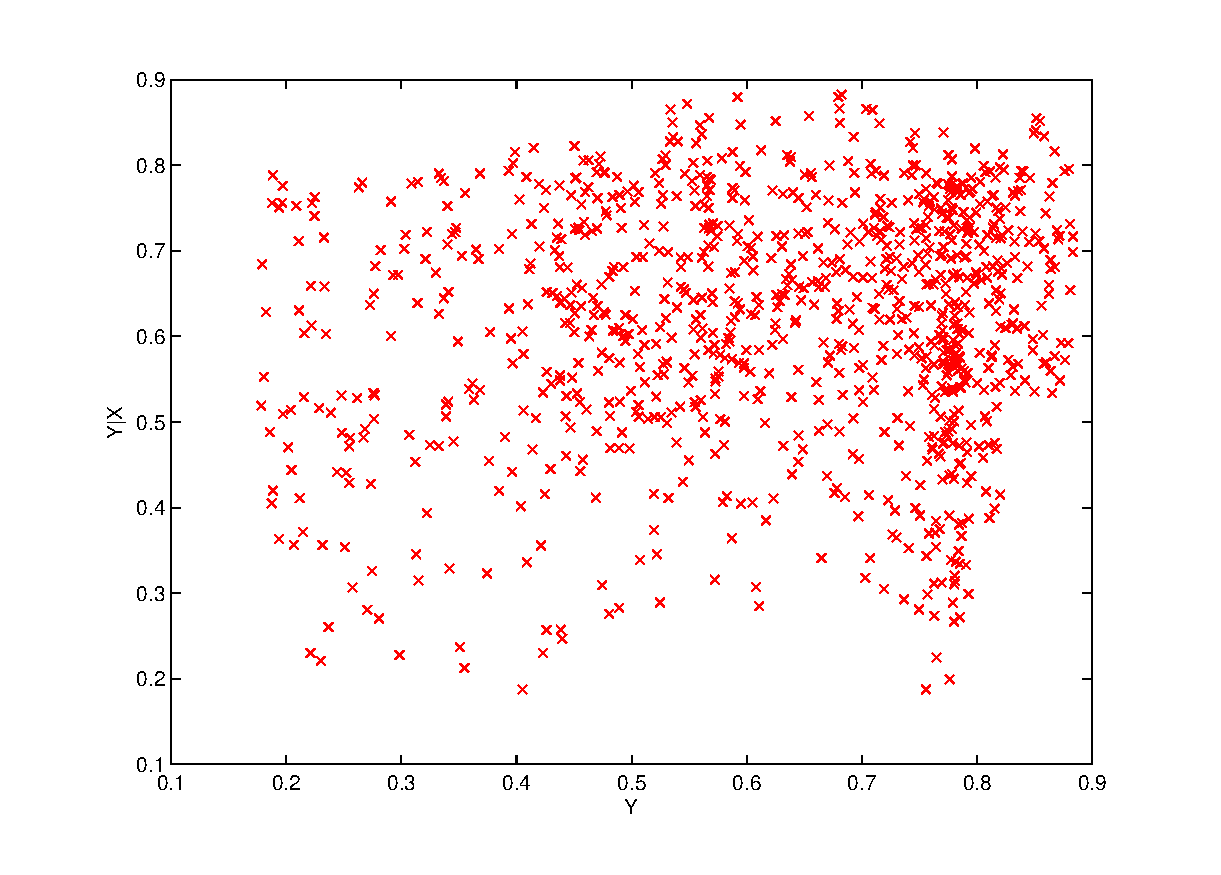
\includegraphics[scale=0.5]{SugFig3_YgX.eps} \\
(b) $C_{YX}$ \\[6pt]
\end{tabular}
\caption{Changing $A$ and $B$.  $C_{XY}$ and $C_{YX}$}
\label{fig1}
\end{figure}
\end{center}
This leads to

\begin{tabular}{c|c|c}
$C_{XY}$ & $C_{YX}$ & $\Delta=C_{YX}-C_{XY}$ \\
\hline \\
0.973921 & 0.110698 & -0.8632
\end{tabular}

But, these are not the only correlations that can be tested:
\begin{center}
\begin{figure}[H]
\begin{tabular}{cc}
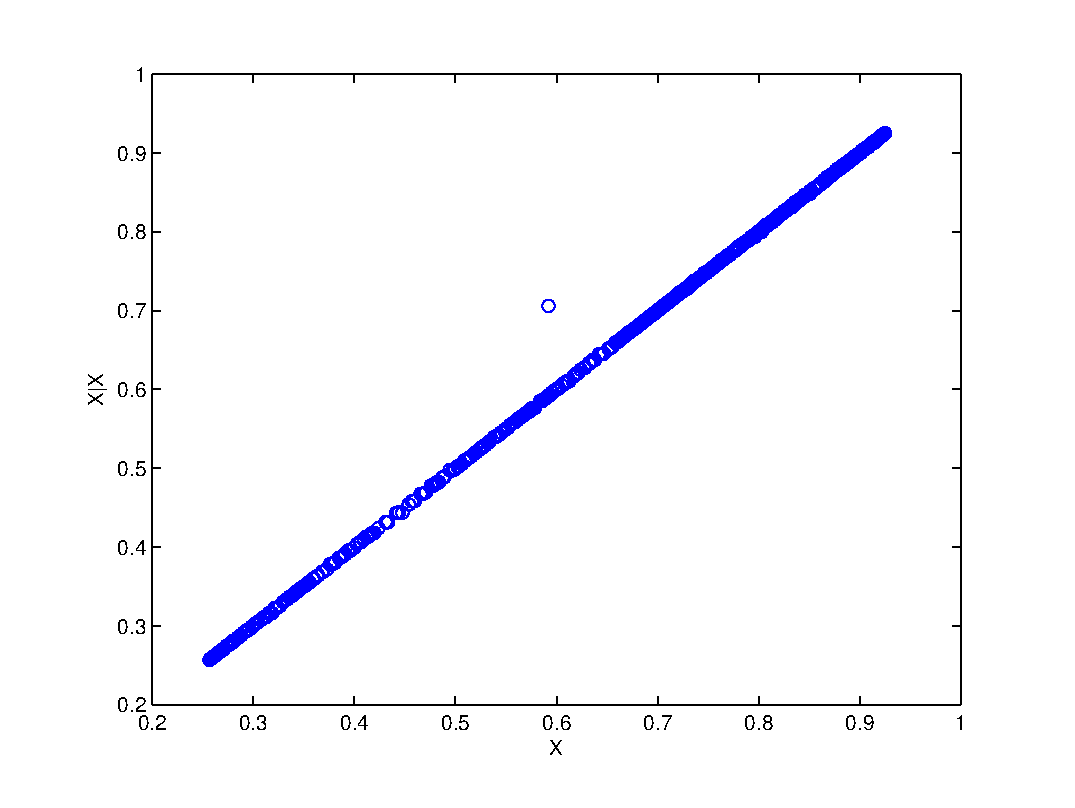
\includegraphics[scale=0.5]{SugFig3_XgX.eps} \\
(a) $C_{XX}$ \\[6pt]
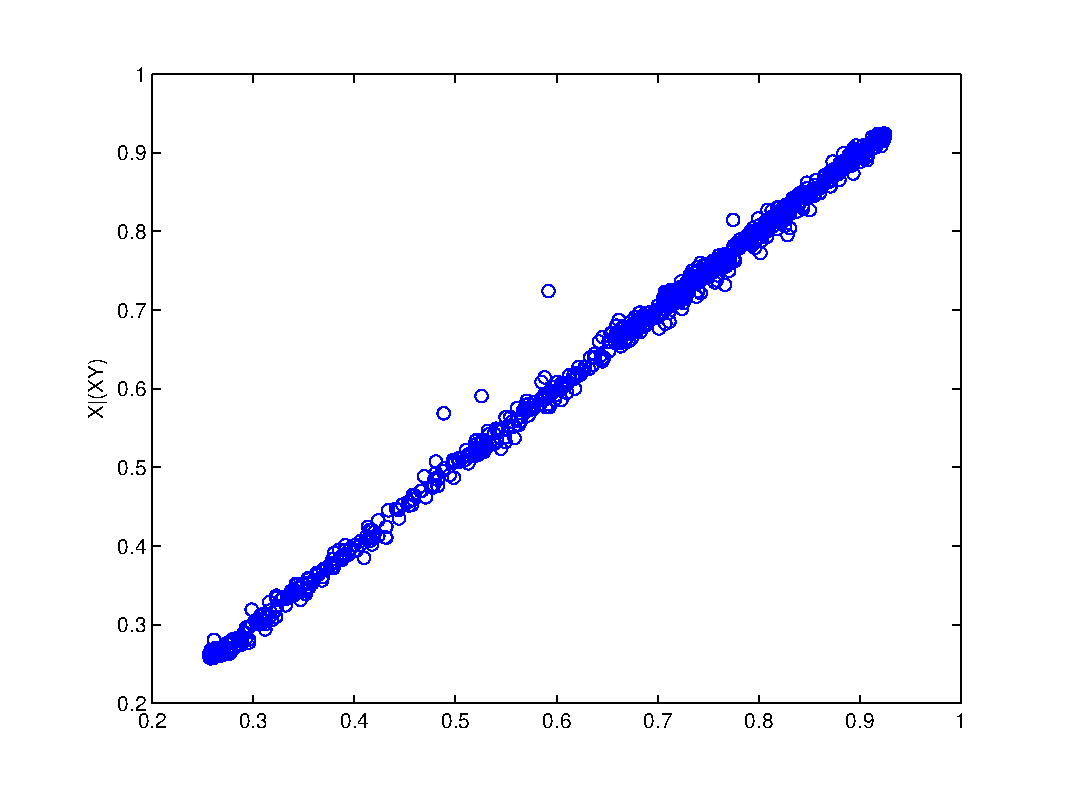
\includegraphics[scale=0.5]{SugFig3_XgXY.eps} \\
(b) $C_{X(XY)}$ \\[6pt]
\end{tabular}
\caption{Changing $A$ and $B$.  $C_{XY}$ and $C_{YX}$}
\label{fig1}
\end{figure}
\end{center}
\begin{center}
\begin{figure}[H]
\begin{tabular}{cc}
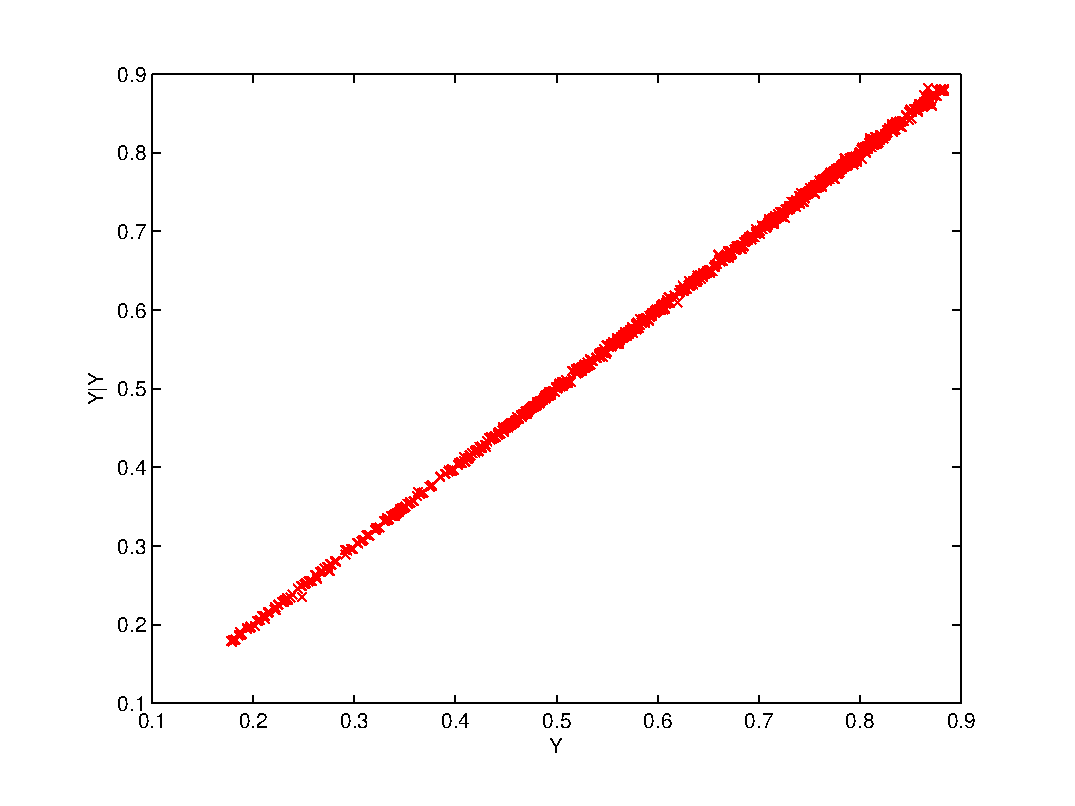
\includegraphics[scale=0.5]{SugFig3_YgY.eps} \\
(c) $C_{XX}$ \\[6pt]
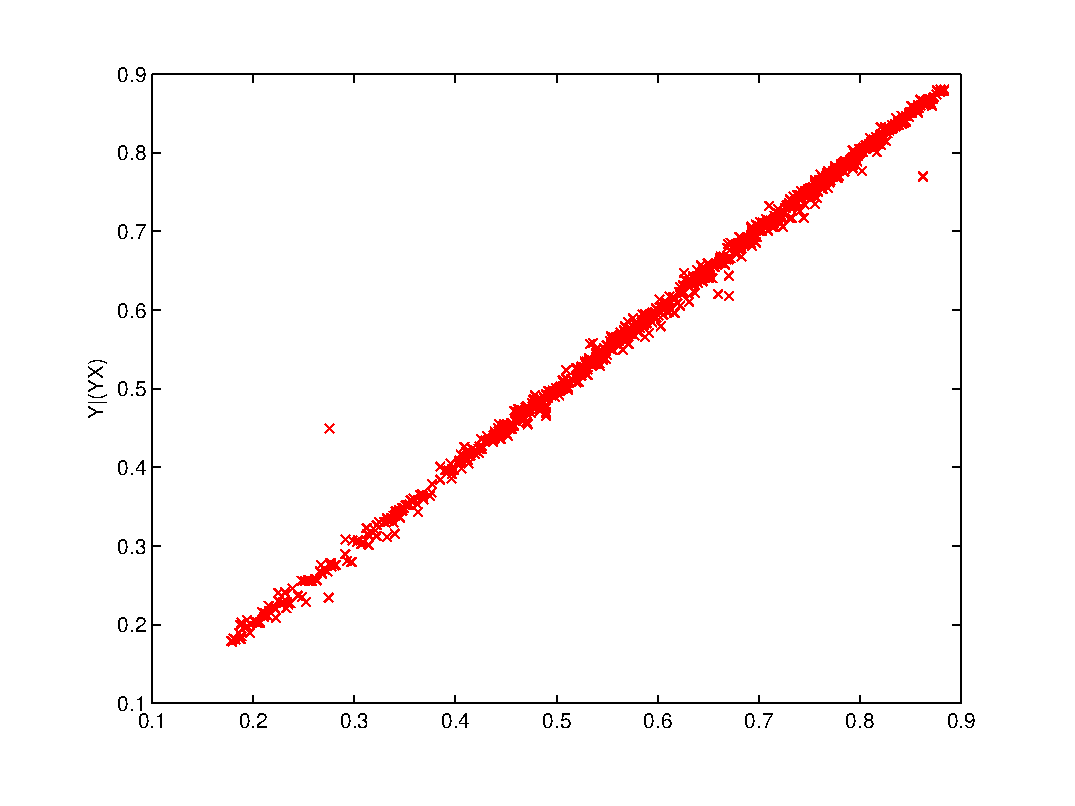
\includegraphics[scale=0.5]{SugFig3_YgYX.eps} \\
(d) $C_{X(XY)}$ \\[6pt]
\end{tabular}
\caption{Changing $A$ and $B$.  $C_{XY}$ and $C_{YX}$}
\label{fig1}
\end{figure}
\end{center}
This leads to

\begin{tabular}{c|c|c|c|c}
$C_{XX}$ & $C_{X(XY)}$ & $C_{YY}$ & $C_{Y(YX)}$ & $\Delta=C_{Y(YX)}-C_{X(XY)}$ \\
\hline \\
0.999841 & 0.998989 & 0.999908 & 0.998693 & -2.9548e-04
\end{tabular}

Consider a comparison of PAI and CCM given the linear example system from above.  
\begin{figure}[H]
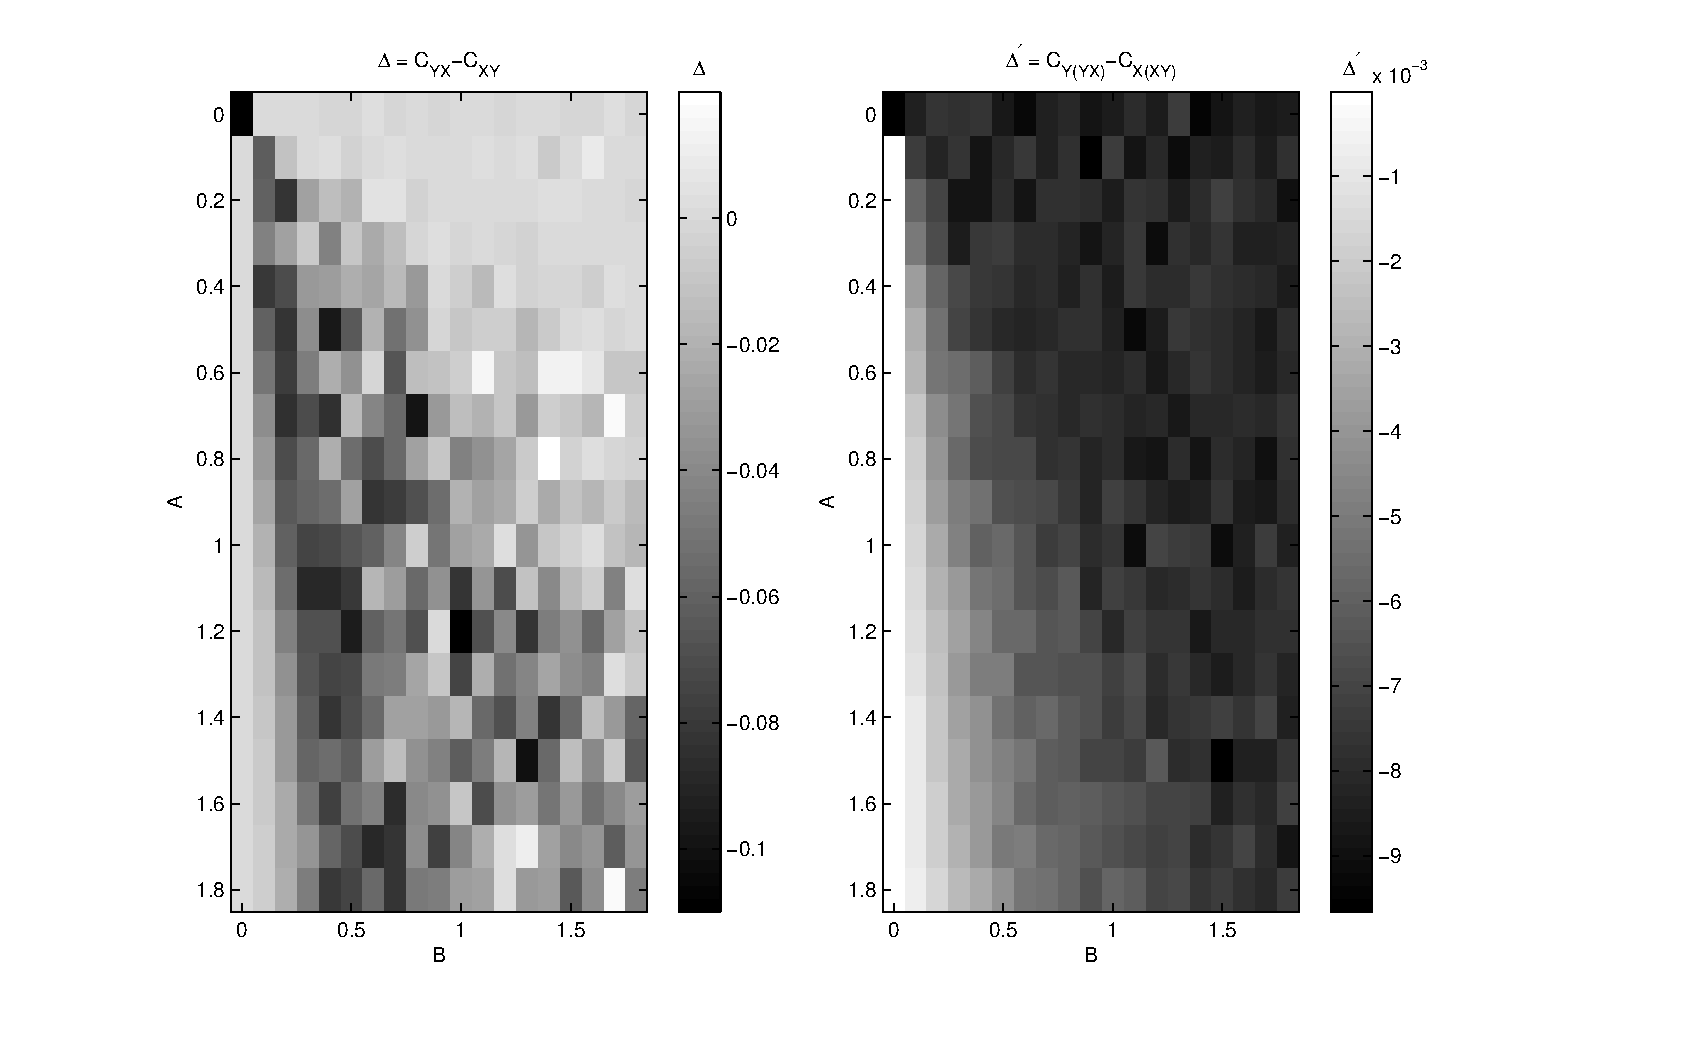
\includegraphics[scale=0.8]{LinearEx_PAItemp.eps} \\
\caption{Changing $A$ and $B$.}
\label{fig1}
\end{figure}



\end{document}

